\documentclass{ltjarticle}
\usepackage{geometry}
\usepackage[dvipdfmx]{graphicx}
\usepackage[colorlinks=true, allcolors=black] {hyperref}
\usepackage{amsmath}
\usepackage{mathtools}
\usepackage{bm}
\usepackage{listings}
\usepackage{array}
\everymath{\displaystyle}
% ページの余白を1.25インチにする
\geometry{
    left=1.25truein,
    right=1.25truein,
    top=1.25truein,
    bottom=1.25truein,
}
%
\begin{document}
\begin{titlepage}
    \begin{center}
        {\Large 令和6年 3月4日}
        \vspace{20truept}

        {\LARGE 修士学位論文}
        \vspace*{180truept}

        {\Huge Biterm Topic Modelを用いた}\par
        {\Huge SNS上の商品レビューに対する}\par
        {\Huge 関連性評価}
        \vspace{160truept}

        {\Large 指導教員:相馬 隆郎 准教授}
        \vspace{30truept}

        {\Large 東京都立大学大学院}
        \vspace{10truept}

        {\Large 電子情報システム工学域}
        \vspace{30truept}

        {\Large 学修番号:22861651}
        \vspace{10truept}
        
        {\Large 氏名:西原涼介}
    \end{center}
\end{titlepage}
\noindent
{\LARGE 論文要旨}
\vspace{20truept}

近年, Amazonや楽天市場などの大手ECサイトをはじめ, 数多くのECサイトが普及しその利用者数は急速に増加している. 
ECサイトの利用者のうち, 約70\%が商品を購入する際にECサイトのレビューを参考にしているとされ, 
その中でも特にレビューの信頼性を重要視している人が多いことが明らかになっている. また, 多くの企業にとってはECサイトの
レビューからユーザーの嗜好や意見を分析し,マーケティングに活用することが重要な課題となっている.そのため,
ECサイトのレビューの信頼性や有用性を評価する評判分析や口コミ分析, レビューを様々なトピックに分類する文書分類に関する
研究が多く行われている. 例えば, Amazonの商品レビューを機械学習を用いて分析し, 他のユーザーにとって
参考になる順に並び替えるシステムの構築及びその評価に関する研究や, グルメサイトの口コミにおいて実名・顕名・匿名
の違いがレビューの信頼性に与える影響についての研究などが挙げられる. 
また近年では, 従来のECサイトや商品のWebページだけではなく, YouTubeのような
動画投稿サイトやX(旧Twitter)やInstagramなどのSNSを自社製品やサービスの宣伝の場として利用している企業が増加している. 
これに伴い, 商品を購入する際にSNSやYouTube上でその商品を宣伝している投稿を参考にしている人も増加している. 
そのため, SNSやYouTube上の広告に対するユーザーのコメントも, 他のユーザーが商品の購入を検討する際の重要な判断
材料になり得ると考えられる. つまり, SNSやYouTube上での商品の宣伝に対するコメントは, ECサイトの商品レビュー
と同等の機能を持ち, その信頼性や有用性が重要視されるため, 同じく評判分析や文書分類の研究の対象になると考えられる. 
例えば, SNSやYouTubeは商品レビューのページとは異なり, 誰でも気軽にコメントを投稿できたり, その投稿内容も自由という特性上, 
商品やサービスに関係ないコメントが多数存在するという問題がある.

そこで, 本研究では分析対象をYouTube上で自社製品やサービスを宣伝している動画に対するユーザーのコメントとし, 
その動画で宣伝している商品やサービスに対しての関連性が高いコメントを抽出するシステムの作成, 及び作成したシステムの人手に対する
精度の検証を目的としている. これにより, ECサイトの商品レビューと同様に他のユーザーが商品の購入を検討する際の重要な判断材料として
扱うことが可能になると考えられる. 

この目的の実現のため, 本研究ではトピックモデルの一種であるBiterm Topic Model(BTM)を用いたトピック抽出, 及び各トピックの生成確率上位の
単語を利用した手法を提案する. BTMは他のトピックモデルとは異なり, 文書全体のバイターム(2単語の対)の共起性を利用してトピックを学習するため, 
YouTubeのコメントのように一文が比較的短い場合でも適切にトピックを推定することが可能であると考えられる. 
以下に本研究の提案手法の概要を述べる. 
はじめに, 商品やサービスの宣伝を行っているYouTube動画に対するコメントをYouTube Data APIを用いて取得し, クリーニング処理や
分かち書きなどの前処理を施す. 次に, 前処理をしたコメント集合にBTMを適用し, 潜在的なトピックの推定と各トピックにおける
生成確率上位の単語を抽出する. そして, 大規模言語モデルであるGPT-4を用いて, 各トピックから抽出した単語を基に文章を自動的に生成する. 
ここで生成した文章はBTMによって推定したトピックに出現しやすい単語を用いているため, 各トピックの代表的な文章であるという仮説を立てることができる. 
つまり, 生成した文章は元のコメント集合に対して代表的であり, 動画内容に関連している文章であるという仮説が立つ. 
その仮説を基に, 各トピックごとに生成した文章と元のコメント文との文章間の類似度を計算し並び替えることで, 本研究の目的である
動画に対して関連性が高い文章の抽出が実現できると考えた. また, 本仮説の妥当性, 及びシステムの精度を検証するために, 人手で
アノテーションしたデータセットとの比較分析を行った. 

実際のYouTubeコメントを本手法に適用し実験を行なった結果, BTMによって商品に関連しているトピック及び単語を適切に抽出することができた. 
また, 人手でアノテーションしたデータと本手法で類似度計算を行ったデータからConfusion Matrixを算出し, 様々な指標で
本手法の性能を評価した. その結果, Precision(適合率)が0.7程度の値を示したことから, 本手法により商品との関連性が高いと予測したコメントのうち
約7割が人手の評価に対して正しく予測できていることが分かった. 
この結果より, 本研究で提案したSNSやYouTubeコメントに対する新たな分析手法の有効性を示すことができた. 


% 目次
\newpage
\tableofcontents
\clearpage

\part{はじめに}
\vspace{10truept}
\section{研究背景}
近年, Amazonや楽天市場などの大手ECサイトをはじめ, 数多くのECサイトが普及し, その利用者も急増して
いる. そして, 商品を購入する際にECサイトのレビューを参考にしている利用者の割合は約70\%と言われていて, そ
の中でもレビューの信頼性を重要視している人が多いことが明らかになっている. また, 多くの企業にとって, ECサイトの
レビューからユーザーの嗜好や意見を分析し,マーケティングに活用することが重要な課題となっている.そのため,
ECサイトのレビューの信頼性や参考になるかどうかを評価する評判分析や口コミ分析, レビューを様々なトピックに分類する文書分類に関する
研究が多く行われている. 例えば, 関連研究の項で詳しく紹介する「機械学習を用いた自然言語処理による商品レビューの評価」[1]では, Amazonの商品レビュー
を機械学習を用いて参考になる順に並びかえるシステムの構築, 及びその評価に関する研究を行っている。
また近年では, 従来のECサイトや商品のWebページ以外にも, YouTubeのような
動画投稿サイトやX(旧Twitter)やInstagramなどのSNSで自社製品・サービスの宣伝を行う企業が増えてきている. 
それにつれて, 商品を購入する際にSNSやYouTube上でその商品を宣伝している投稿を参考にしている人も増加している. 
そのため, SNSやYouTube上の広告に対するユーザーのコメントも, 他のユーザーが商品の購入を検討する際の重要な判断
材料になり得ると考えられる. つまり, SNSやYouTube上での商品の宣伝に対するコメントは, ECサイトのレビュー
と同等の機能を持ち, その信頼性や参考になるかどうかが重要になるため, 
評判分析や文書分類の研究の対象になると考えられる. ここで, SNSやYouTubeは商品レビューのページとは異なり, 
誰でも気軽にコメントを投稿できたり, その投稿内容も自由という特性上, 商品やサービスに関係ないコメントが
多数存在する.

そこで, 本研究では分析対象をYouTube上で自社製品やサービスを宣伝している動画に対するユーザーのコメントとし, 
トピックモデルの一種であるBiterm Topic Modelによる商品に関するトピック抽出を用いて, 
その動画に対するユーザーのコメントから, 宣伝している商品やサービスに対して関連性が高いコメントを
抽出するシステムの作成, 及び作成したシステムの人手に対する精度の検証を行った. 

本論文の第Ⅰ部では, ECサイトのレビューにおける評判分析やトピックモデルを用いた文書分類に関する関連研究の紹介, 
また本研究の研究目的を明確に説明する.
第Ⅱ部では, 本研究で用いる二つのトピックモデルの説明, 及び提案手法のシステムや実装方法について説明する.
第Ⅲ部では, 実際のYouTube上の動画に対するコメントを用いた実験結果を述べる.
第Ⅳ部では, 実験結果をもとに考察した提案手法の有効性や将来性について述べる. 

\newpage
\section{関連研究}
本研究を進めるにあたり, 研究テーマの方向性決めや研究課題の発見, 及び本研究で用いている技術に関して参考にした
論文を4つ紹介する. 
\subsection{機械学習を用いた自然言語処理による商品レビューの評価(市川(2021)[1])}
市川(2021)は, ユーザーが商品レビューを読んで参考になったかどうかを評価する機能が備わっていない
ECサイトの場合に, 数多くあるレビューから参考になる情報を探す必要がある問題に着目し, 
機械学習を用いた自然言語処理の手法で分析, 評価を行い, レビューを参考になる順番に並び替える
システムの構築を目的としている. そして並び替えた順番が正しいかどうかを評価するために, クイックソートを利用した
新しい評価法であるQE法を提案している. 

図\ref{fig:関連研究1システム概要図}は市川(2021)で提案されている, レビューを参考になる順番に並び替えるシステムの概要図である. はじめに, 
インターネット経由でAmazonの商品レビューのデータ取得し, 学習用データと評価データに分ける. 学習段階では, レビュー文章の
正規化や各前処理を施し, 教師データとして準備する. 
この研究では, 全角数字やアルファベットを半角に変換したり, 
数字は全て0に置換, アルファベットは全て小文字に変換などの正規化を行っている. また, 日本語形態素解析システムであるMeCab
を用いて形態素解析を行い, 品詞ごとに``\_''で分割する. その後, 活用語の原型への変換, 及びストップワード除去を行っている.
例えば, 「ロボットは24時間働けるのでAIに仕事をとられる.」という文章の場合, 正規化と前処理を施すことで, 
「ロボット\_0\_働ける\_ai\_仕事\_とる.」となる. この一連の処理を学習用データに施した後, 機械学習の際に用いる素性
の抽出を行う. 
\begin{figure}[h]
    \centering
    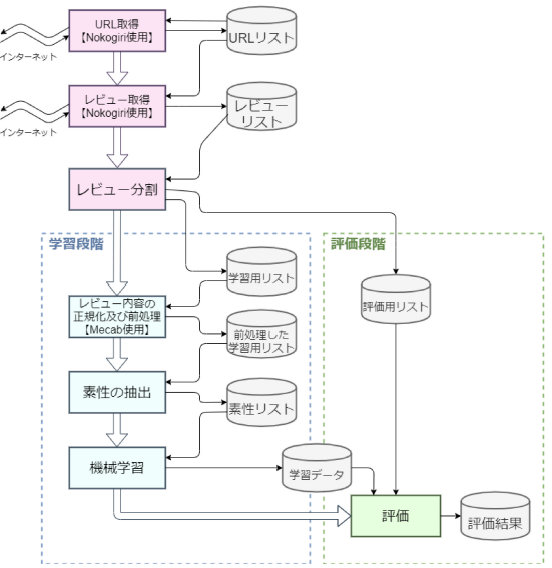
\includegraphics[width=10cm]{images/system1.png}
    \caption{システム概要図 (出典:市川[1] p.85)}
    \label{fig:関連研究1システム概要図}
\end{figure}
市川(2021)はレビューを参考になる順序に並べ替えることが目的のため, 素性には単語の出現頻度を用いている. 
目的変数をレビューが参考になる確率$P$とし, 抽出した素性を用いてロジスティック回帰により学習する. 
ロジスティック回帰のモデル式は式(\ref{equation:ロジスティック})で示される. $\theta_i$は素性の重み, $N$は素性の数を表している. 
\vspace{5truept}

\begin{equation}
    P=\dfrac{1}{1+exp(\theta_0x_0+\theta_1x_1+\cdots+\theta_Nx_N)}
    \label{equation:ロジスティック}
\end{equation}
\vspace{5truept}

次に学習したモデルを用いて, 評価用データに対して実験を行ない, 提案システムの精度を検証している. 
この研究の提案システムの精度の評価は, 実際の商品ページのレビューの並び順との一致率で評価している. 
正解の並び方を$L_R$, 提案システムによる並べ方を$L_P$としたとき, それぞれの要素の一致率を$P_{match}$としている. 
例えば, 以下の並び方のとき, $P_{match}=100\%$となり最も良い結果となる. 
\begin{align}
    L_R:\{1,2,3,4,5\}\notag\\
    L_P:\{1,2,3,4,5\}\notag
\end{align}
しかし, 以下のように並び方の評価としては良い結果と言える場合でも, 5件のレビュー中1件のみ一致していることになり, 
$P_{match}=20\%$と低い結果になる. 
\begin{align}
    L_R:\{1,2,3,4,5\}\notag\\
    L_P:\{4,1,2,3,5\}\notag
\end{align}

このように正しい評価が行えない場合を解決するため, この研究ではクイックソートを利用した新しい評価法のQE法(Quicksort Evaluation method)
を提案している. QE法ではピボットを中央値とし, 昇順にするために要素を入れ替えた回数$S_{count}$と, 要素数における最大の入れ替え回数
$S_{max}$を用いた式(\ref{equation:QE法})により, 評価値$P_{QE}$を求めている. なお, $S_{max}$は全ての要素が逆順の場合にクイックソートで
昇順に入れ替えた回数である. 
\vspace{5truept}

\begin{equation}
    P_{QE}=1-\dfrac{S_{count}}{S_{max}}
    \label{equation:QE法}
\end{equation}
\vspace{5truept}

実際の商品レビュー52,403件を取得し, そのうち51,403件を学習用データ, 1,000件を評価用データに分けて実験を行い, 提案システムの
精度を評価した結果を表\ref{table:関連研究1結果}に示している. 
ここで, 登場回数$F$とは学習の素性とするか決定するための単語の出現回数である. 
表\ref{table:関連研究1結果}から, $F=5000$, 学習率$\eta=1.7$のときに評価値$P_{QE}=0.814$と最大になる. したがって, この論文で提案しているシステムは
レビューを参考になる順序に並び替える手法として有効であると言える. 

しかし, 市川(2021)ではAmazonの商品レビューを分析の対象としていて, 素性には単語の出現頻度を用いているため, 
提案システムが成り立つにはしっかり商品をレビューしている文章を学習させる必要がある. そのため, この論文で提案されているシステム
ではYouTubeで商品を宣伝している動画や, SNSの投稿に対するコメントを学習させた場合に上手く学習できなかったり, 精度が悪くなってしまう
ことが考えられる. なぜならば, YouTubeの動画やSNSの投稿に対するコメントというのは誰でも気軽にでき, 内容も自由であるため, 
商品のレビューのようなコメントの数がAmazonの商品レビューに比べると少ないからである. また, 一文の長さも短いことが多く, 素性となり得る単語の抽出
も難しいと考えられる. そこで, 本論文ではそのような問題を解決するための手法を第Ⅱ部で提案する.
\begin{table}
    \centering
    \caption{登場回数と学習率の組み合わせごとの評価値$P_{QE}$ (出典:市川[1] p.91)}
    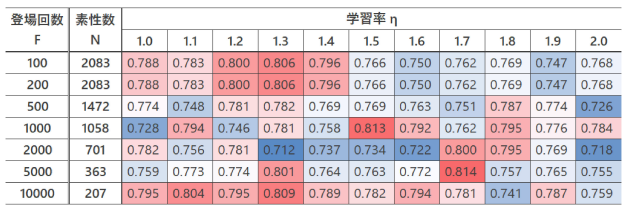
\includegraphics[width=14cm]{images/table1.png}
    \label{table:関連研究1結果}
\end{table}
\vspace{20truept}

\subsection{単語の出現頻度と類似性に基づいたトピックモデル洗練化手法(東(2019)[2])}
東(2019)では, 第Ⅱ部で後述するトピックモデルの一種のLatent Dirichlet Allocation(以下LDA)を自然言語文書に適用する際の
改善案を提案している. 
通常, トピックモデルを自然言語文書に適用する際には, 前処理として分類に不必要なストップワードの除去を行うことが多いが, 
一般的にストップワードリストに含まれている単語を除去するだけでは, 特定の文書にのみ頻出する特徴的な単語
を除去することが出来ず, トピックモデルの精度に影響を及ぼすという問題が存在する. 
また, トピックモデルによって分類したトピックには, 類似したトピックが複数出現し, 
分類の精度が下がるという問題も存在する. 

そこで東(2019)では, 前処理として分析対象としている文書から適切なストップワードリストを作成する方法を提案している. 
また, トピックモデルを適用後の後処理として, トピックを構成している単語の類似度からトピック間の距離を算出し, 
類似しているトピックを統合することでより正確なトピック分類を可能にする手法を提案している. 図\ref{fig:関連研究2提案手法}は提案手法の全体像である. 
\begin{figure}[h]
    \centering
    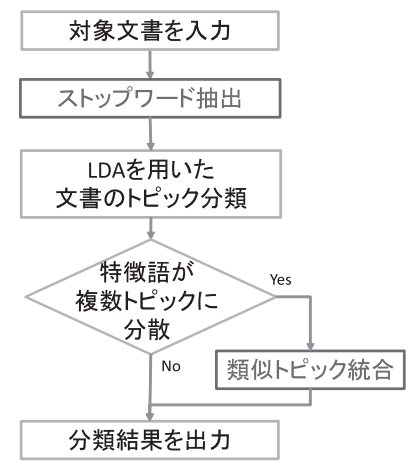
\includegraphics[]{images/fig2.png}
    \caption{提案手法の流れ (出典:東[2] p.27)}
    \label{fig:関連研究2提案手法}
\end{figure}

ストップワードリストを作成する手順を図\ref{fig:関連研究2ストップワード}で示している. この手法では, まず対象としている文書全体に対して出現率が高い
単語をストップワードとして抽出する. 出現率の算出にははDF(Document Frequency)を用いている. DFとは, 文書全体に対して
ある単語Tが含まれる文書数のことであり, 事前に設定した閾値よりも高いDF値を持つ単語をストップワードリストに加える. 
次に, 抽出した単語と意味的に類似している単語をさらにストップワードとしてリストに加える. 
word2vecを用いて文章中の各単語を周辺の単語から学習し, 単語の分散表現を得て単語間の類似度を算出する.  
それによりある単語Tの類似単語を抽出することができ, ある閾値以上の類似度を示した単語を全てストップワードリストに加える. 
これにより, DF値が高くない場合でも文書の特徴を表しにくい単語をストップワードリストに加えることが可能になる. 
\begin{figure}[h]
    \centering
    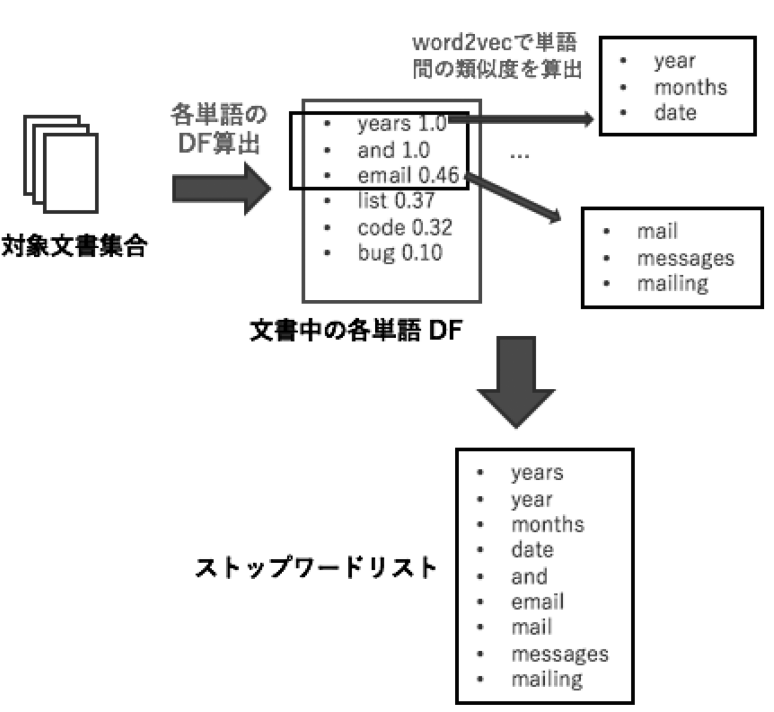
\includegraphics[]{images/fig3.png}
    \caption{ストップワード抽出手法の流れ (出典:東[2] p.27)}
    \label{fig:関連研究2ストップワード}
\end{figure}

トピックモデル適用後の後処理では, 分類結果に似たよったトピックが存在する場合にそれらのトピックを統合する処理を行うことを提案している. 
類似トピックの判断基準には, TF-IDF cos類似度推定法が用いられている. これは, cos類似度の計算に使用する
ベクトルの成分をTF-IDFで算出したものにした手法である. この研究では, 分類した各トピックの単語集合に対して
TF-IDF cos類似度を利用したクラスタリングを行い, その結果に従ってトピックを統合する手法を提案している. 

以上の提案手法をLDAのよるメーリングリストのトピック分類に適用し, 評価項目に基づいて比較することで提案手法
の有効性の評価を行っている. 評価項目として, 一般的なストップワードリストを用いた手法と提案手法を比較している. 
また, 後処理として類似トピックの統合を行った場合についても比較を行っている. 
トピック分類の正確さを評価する指標として, 適合率, 再現率, それらの調和平均のF値を採用している. 
実験結果を表\ref{table:関連研究2結果}に示している. 表\ref{table:関連研究2結果}より, LDAを自然言語に適用したトピック分類では, 前処理としてストップワード除去
を行うことで分類精度が大幅に向上していることが分かる. また, 一般的なストップワードリストを用いた場合と提案手法
によるストップワードリストを用いた方法を比較するとF値が向上している. また, 後処理を行った場合のF値はさらに向上している
ことから, トピック分類の正確性を向上させる提案手法の有効性を確認できている. 

本研究ではトピックモデルの分類精度よりも抽出する単語の質を重視しているため, 東(2019)で提案されているストップワードリスト
作成方法を用いると抽出したい単語をストップワードリストに加えてしまう恐れがある. 
また, 本研究で分析の対象としているYouTubeのコメントは, 書き言葉よりも話し言葉で書かれていたり, 若者言葉が使われていることが多く, 
一般的なストップワードリストだけでは不要な単語を除去することが困難である. そのため, 前処理で形態素解析を行い, 特定の品詞のみ抽出
してストップワードとして除去する, または特定の品詞のみでトピック分類を行う手法で実験を行った. 
\begin{table}
    \centering
    \caption{ストップワード数($\#N$), 適合率, 再現率, F値の結果 (出典:東[2] p.30)}
    \vspace{5truept}
    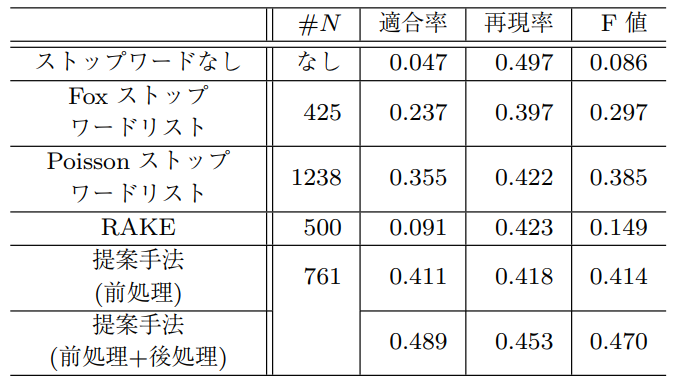
\includegraphics[]{images/table2.png}
    \label{table:関連研究2結果}
\end{table}
\vspace{10truept}

\subsection{テキストマイニングを用いた口コミ分析による点数評価の信頼性確認手法(谷口(2017)[3])}
谷口(2017)は商品に対して点数評価を加えたレビューを行える口コミサイトに関して, 平均値や点数の分布が示されているなどの
メリットがあることに対し, 点数の信頼性に疑問を抱く購入検討者が多い問題に着目している. 
そこで, カメラを購入した顧客からの点数評価とレビューを用いて, 点数評価の信頼性を確認する手法を提案している. 

谷口(2017)はまずSonyの製品サイト上のカメラに関するレビューから, 5段階の総合評価の点数を集計している. 
次に, カメラの特徴(画質・機能・デザインなど)に関する点数評価を集計し, その結果を表\ref{table:関連研究3表1}に, 
総合評価で5を付けた人の各項目の点数評価の集計結果を表に示している. 
谷口(2017)は, この集計結果より総合評価5を付けている人でも全ての項目で満足しているわけで

\begin{table}[h]
    \centering
    \caption{各項目の点数評価 (出典:谷口[3] p.2)}
    \vspace{5truept}
    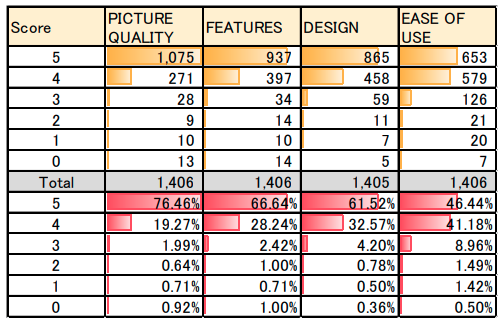
\includegraphics[width = 10cm]{images/関連研究3表1.png}
    \label{table:関連研究3表1}
\end{table}
\vspace{20truept}

\newpage
\begin{table}[h]
    \centering
    \caption{総合評価5の各項目の点数評価 (出典:谷口[3] p.2)}
    \vspace{5truept}
    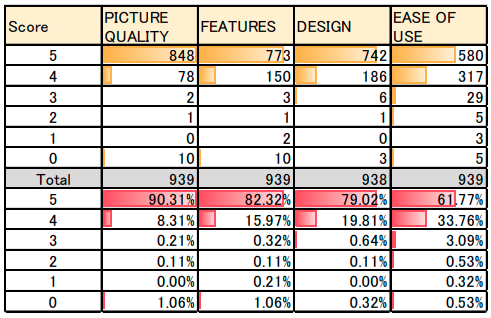
\includegraphics[width = 10cm]{images/関連研究3表2.png}
    \label{table:関連研究3表2}
\end{table}
\vspace*{20truept}

\noindent
はないことや, 逆に評価項目にはない部分で製品に対して満足している可能性などに言及している. 
この点数評価の信頼性を確認するため, 製品に対するレビューをテキストマイニングにて分析し, 
Positive, Neutral, およびNegativeの表現を抽出する感性評価を行っている. 
総合評価の各点数ごとのレビューから各感性の出現頻度をカウントした結果が表\ref{table:関連研究3表3}である. 
表\ref{table:関連研究3表3}より, 総合評価4ではNeutralに分類されている文章が9割を超えていることや, 総合評価5では
半数がNeutralを示し, Negativeと判定された口コミが0件であることが分かる. 
この結果より, 谷口(2017)は総合評価は妥当な点数であるといえることや, 
総合評価が満点であっても全ての項目に対して満足しているわけではない場合もあることを明らかにしている. 

総合評価5のときNegativeが0件であることから点数評価の妥当性を判断できるが, Neutralに分類された文書
が多い総合評価4に妥当性があるかどうかは判断が難しいと感じた. また, 谷口(2017)の研究は点数評価に対する信頼性を
評価しているため, 文書自体の信頼性については確認されていない. 本研究では, Positive, Negativeなどの評価表現
の有無に依存せずに文書の分類(商品との関連性の有無)を行える手法を提案する. 


\begin{table}[h]
    \centering
    \caption{総合評価と口コミ分析の感性評価 (出典:谷口[3] p.2)}
    \vspace{5truept}
    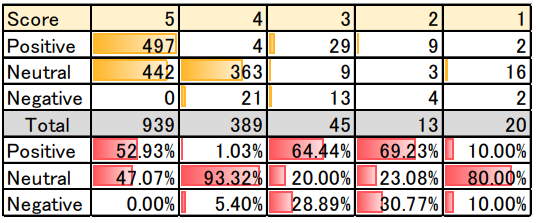
\includegraphics[width = 10cm]{images/関連研究3表3.png}
    \label{table:関連研究3表3}
\end{table}

\newpage
\subsection{グルメサイトにおけるクチコミの信頼性確保に関する一考察(吉見(2014)[4])}
吉見(2014)はグルメサイトの「食べログ」で所謂やらせのレビューが行われていた問題によって口コミの信頼性が揺らいでいる
問題に着目し, 実名・顕名・匿名といった口コミの差異がその信頼性に与える影響について検討している. 
各項目は表\ref{table:関連研究4表1}の定義に従って分類されている. 
吉見(2014)は以下のリサーチ・クエスチョンについてテキストマイニングの手法を用いた分析を行っている. 
\begin{quote}
    実名のグルメサイトは「長期的関係による評判」を重視し, 匿名・顕名のグルメサイトは
「不完備情報による評判」を重視している. (吉見 2014, p.3)
\end{quote}
さらに, 実名の特徴として評判の種類が「長期的関係」であること, 匿名と顕名については「不完備情報」
であると仮定している(吉見 2014, 表3). 
匿名・顕名のグルメサイトとして「食べログ」を, 実名のグルメサイトとして「Rettyグルメ」を対象に
実験を行った結果, 投稿数と1投稿あたりの文字数は顕名>匿名>実名の順に小さく傾向があることを明らかにしている. 
また, 全体の1割以上の投稿に現れている単語を対象に共起ネットワーク分析を行った結果, 同様に顕名>匿名>実名の
順に密から疎に変化していることが分かり, この結果からも実名の投稿が簡素であるという結果を明らかにしている
(図\ref{fig:顕名}, 図\ref{fig:実名}). 

以上の実験結果より, 吉見(2014)は実名の投稿が「長期的な関係による評判」に依拠していて, 
レビュアーへの信頼を補完しているため詳細なクチコミを必要としていないと考察している. 
また匿名・顕名の投稿は「不完備情報による評判」に依拠していて, 
他のユーザーからの信頼を獲得するために比較的詳細なクチコミを求められていると考えている. 
そのため, リサーチクエスチョンは支持されると結論付けている. 

本研究で扱うYouTubeの動画に対するコメントは匿名・顕名であり, 信頼を獲得するにはある程度詳細な情報が求められるが, 
YouTubeの特性上, 誰でも自由に投稿できるため商品に対する詳細なレビューはかなり少ない. 
そのため, 本研究では比較的文章が短い文書集合に対してでも適切に分析することが可能であると考えられる
Biterm Topic Model(Xiaohui Yan 2013)を用いる手法を提案している. 
\begin{table}[h]
    \centering
    \caption{匿名・顕名・実名の分類 (出典:吉見[4] p.2)}
    \vspace{5truept}
    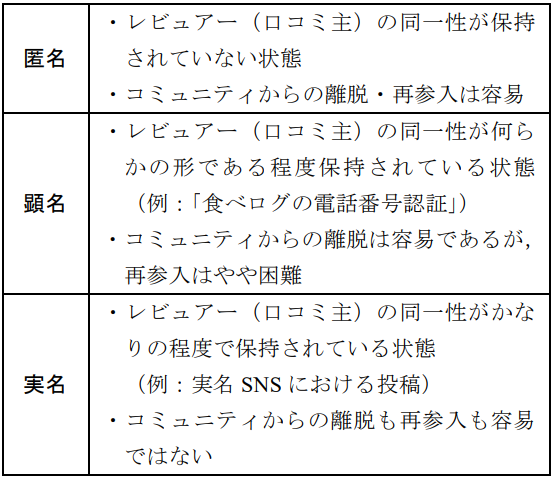
\includegraphics[width = 10cm]{images/関連研究4表1.png}
    \label{table:関連研究4表1}
\end{table}
\newpage
\begin{figure}[h]
    \centering
    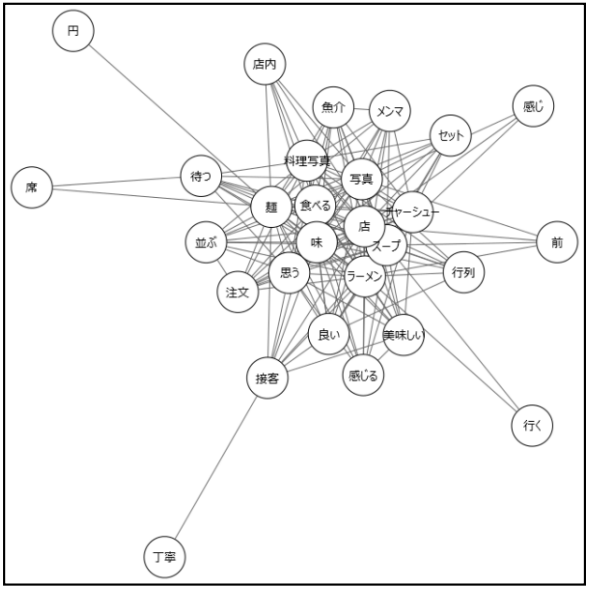
\includegraphics[width=6.5cm]{images/顕名のクチコミ.png}
    \caption{顕名のクチコミ (出典:吉見[4] p.4)}
    \label{fig:顕名}
\end{figure}
\begin{figure}[h]
    \centering
    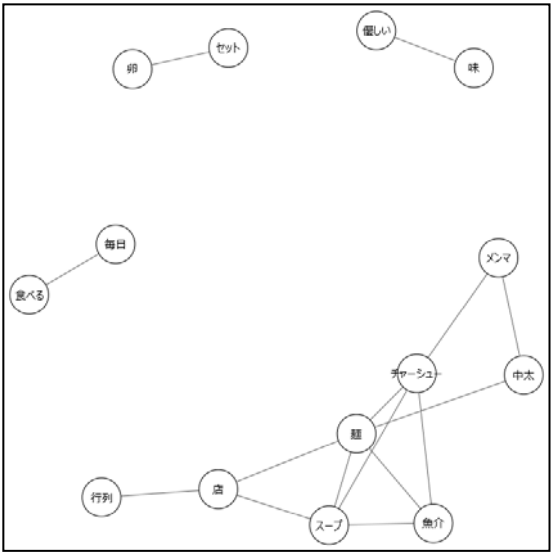
\includegraphics[width=6.5cm]{images/実名のクチコミ.png}
    \caption{実名のクチコミ (出典:吉見[4] p.4)}
    \label{fig:実名}
\end{figure}


\section{研究目的}
前項までの関連研究を踏まえた上で, 本研究の研究目的を明らかにする. 本研究ではYouTube上で商品や
サービスを宣伝している動画に対する視聴者のコメントを分析対象とする. 対象としているコメントのうち, その動画で紹介している商品・
サービスと関連性が高いコメントを抽出するシステムの作成を目的としている. [1]でレビューを参考になる順序に並び替えているように, 
本研究では後述する提案手法により商品との関連性が高い順にコメントを並び替え, 他のユーザーがその商品の購入を検討する際に参考にするコメント
を取得しやすいシステムの作成を目指す. また, 作成したシステムにより抽出した商品との関連性が高いコメントが, 人手の評価に対してどれほどの精度
で抽出できているかを評価し, 最終的な提案手法の精度としている. 

\newpage
\part{提案手法}
第Ⅱ部では本研究の提案手法, 及び提案手法で用いている主要な技術について説明する. 
\section{トピックモデル}
提案手法の説明に先立ち, 本提案手法において主要な技術であるトピックモデルについて説明する. 
トピックモデルとは一つの文書が複数のトピック(主題)を持つと仮定する確率生成モデルである. 
トピックモデルは多くの分野で幅広く活用されており, 例えば文書集合を解析してカテゴリやトピックごとに分類したり, 
顧客からのフィードバックやレビューを解析して商品やサービスに関する主要な問題点や改善点を特定したり, 
生物医学研究では疾患や生物学的プロセスに関連するパターンを特定することに用いられている. 
以下にトピックモデルの概要を示す. 一つの文書が一つのトピックを持つと仮定している「混合ユニグラムモデル」では文書集合全体で一つのトピック
分布があるのに対して, トピックモデルでは文書ごとにトピック分布$\boldsymbol{\theta}_d=(\theta_{d1},\cdots,\theta_{dK})$
が存在する. ここで, $\theta_{dk} = p(k|\boldsymbol{\theta}_d)$は文書$d$の単語にトピック$k$が割り当てられる確率であり, 
$\theta_{dk}\geq0,\sum_{k=1}^K \theta_{dk}=1$を満たす. 
このトピック分布$\boldsymbol{\theta}_d$に従って文書$d$のそれぞれの単語にトピック$z_{dn}$が割り当てられる. 
そして割り当てられた各トピックの単語分布$\boldsymbol{\phi}_{z_{dn}}$に従って単語が生成される. 
ここで, トピックごとの単語分布は$\boldsymbol{\Phi}=(\boldsymbol{\phi}_1, \cdots, \boldsymbol{\phi}_K)$と表せ, 
$\boldsymbol{\phi}_k=(\phi_{k1}, \cdots, \phi_{kV})$はトピックkの単語分布を表す. 
$\phi_{kV}=p(v|\boldsymbol{\phi}_k)$はトピック$k$で単語$v$が生成される確率
($\phi_{kv}\geq0, \sum_{v=1}^V \phi_{kv}=1$)を表している.  
単語の生成過程を図\ref{fig:生成過程}に, 表\ref{table:記号}に4節で用いている記号を示す. 文書ごとのトピック分布$\boldsymbol{\theta_d}$及びトピックごとの単語分布$\boldsymbol{\phi_k}$
はカテゴリ分布のパラメータであるため, その共役事前分布であるディリクレ分布から生成されると仮定している. 
\begin{table}[h]
    \caption{4節で用いる記号}
    \vspace{5truept}

    \centering
    \begin{tabular}{ll}
        \hline
        記号 & 説明 \\
        \hline\hline
        $D$ & 文書数\\
        $N_d$ & 文書$d$に含まれる単語数\\
        $V$ & 文書集合に現れる単語の種類数\\
        $\boldsymbol{W}$ & 文書集合\\
        $\boldsymbol{w}_d$ & 文書$d$\\
        $w_{dn}$ & 文書$d$の$n$番目の単語\\
        $K$ & トピック数\\
        $N_k$ & 文書集合全体でトピック$k$が割り当てられた単語数\\
        $N_{dk}$ & 文書$d$でトピック$k$が割り当てられた単語数\\
        $N_{kv}$ & 文書集合全体で語彙$v$にトピック$k$が割り当てられた単語数\\
        $\theta_{dk}$ & 文書$d$でトピック$k$が割り当てられる確率\\
        $\phi_{kv}$ & トピック$k$のとき語彙$v$が生成される確率\\
        \hline
    \end{tabular}
    \label{table:記号}
\end{table}

\newpage
% \begin{enumerate}
%     \item for トピック $k=1, \cdots, K$
%     \begin{enumerate}
%         \item 単語分布を作成 $\boldsymbol{\phi}_k\sim \textrm{Dirichlet}(\beta)$
%     \end{enumerate}
%     \item for 文書 $d=1, \cdots, D$
%     \begin{enumerate}
%         \item トピック分布を生成 $\boldsymbol{\theta}_d\sim \textrm{Dirichlet}(\alpha)$
%         \item for 単語 $n=1, \cdots, N_d$
%         \begin{enumerate}
%             \item トピックを生成 $z_{dn}\sim \textrm{Categorical}(\boldsymbol{\theta}_d)$
%             \item 単語を生成 $w_{dn}\sim \textrm{Categorical}(\boldsymbol{\phi}_{z_{dn}})$
%         \end{enumerate}
%     \end{enumerate}
% \end{enumerate}
\fboxsep = 20pt
\begin{figure}[h]
    \centering
    \fbox{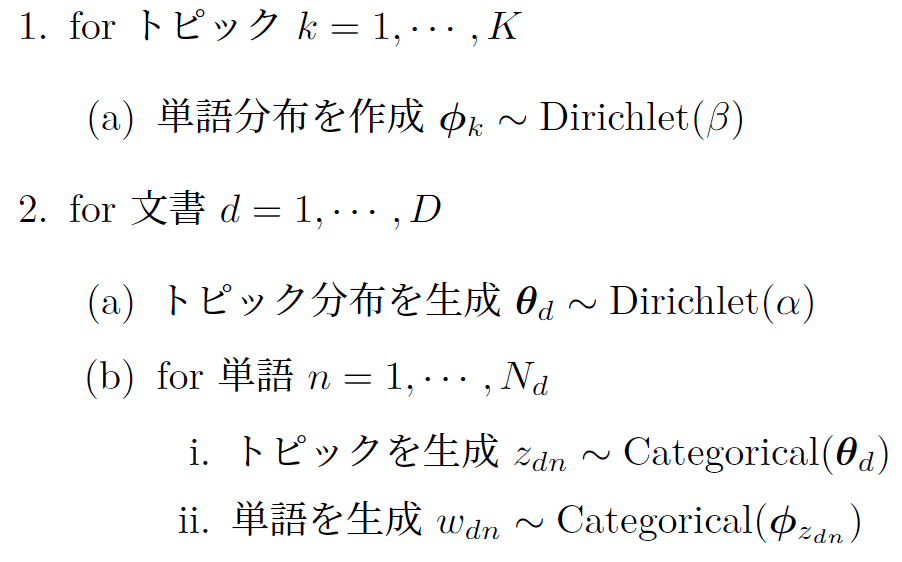
\includegraphics[width = 9cm]{images/生成過程.png}}
    \caption{トピックモデルの生成過程}
    \label{fig:生成過程}
\end{figure}
\vspace{10truept}

同一の文書に含まれる単語でも, 異なるトピックが割り当てられることがあるため, 一つの文書が複数のトピックを持つことが可能である. 
また, 語彙ごとにトピックが割り当てられるわけではなく, 単語ごとにトピックが割り当てられるため, 同じ語彙でも異なるトピック
が割り当てられる可能性も存在する. 
また, トピックモデルは単語にトピックを割り当てる, または単語をクラスタリングするモデルと考えることもできる. 
トピック分布$\boldsymbol{\theta_d}$と単語分布集合$\boldsymbol{\Phi}$が与えられたときの文書$\boldsymbol{w}_d$
の確率は式(\ref{equation:トピックモデル})で表せられる.
\vspace{10truept}

\begin{equation}
    p(\boldsymbol{w}_d|\boldsymbol{\theta}_d,\boldsymbol{\Phi})=\prod_{n=1}^{N_d}\sum_{k=1}^{K} p(z_{dn}=k|\boldsymbol{\theta}_d)p(w_{dn}|\boldsymbol{\phi}_k)=\prod_{n=1}^{N_d}\sum_{k=1}^{K} \theta_{dk}\phi_{kw_{dn}}
    \label{equation:トピックモデル}
\end{equation}
\vspace{10truept}

図\ref{fig:グラフィカルモデル1}にトピックモデルのグラフィカルモデルを示す. グラフィカルモデルとは, 生成モデル内の変数の依存関係を直感的に理解できるように
描いた表現方法である. ここで, 色付きの円は観測変数, 白の円は未知変数を表している. 四角は繰り返しを表し, 右下の数字は
繰り返し回数を表している. また, 右側の四角は単語分布$\boldsymbol{\phi}$がトピック数$K$あることを表している. 
左外側の四角は文書数$D$を, 左内側の四角は各文書に$N$単語含まれることを表している. 
$\alpha$はトピック分布のハイパーパラメータ, $\beta$は単語分布のハイパーパラメータを表している. 
このグラフィカルモデルより, トピック分布$\boldsymbol{\theta}$が文書ごとに存在し, トピック$z$が単語ごとに存在することが
直感的に理解することができる. 
\begin{figure}[h]
    \centering
    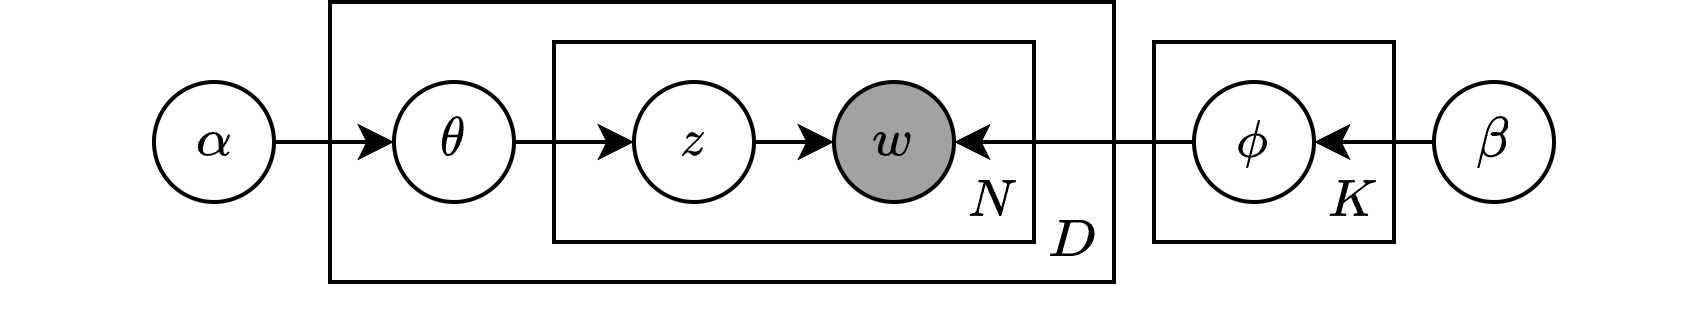
\includegraphics[width = 14.6cm]{images/トピックモデルグラフィカルモデル.drawio.png}
    \caption{トピックモデルのグラフィカルモデル表現}
    \label{fig:グラフィカルモデル1}
\end{figure}


\newpage
\subsection{Latent Dirichlet Allocation}
トピックモデルの代表的な手法に潜在ディリクレ配分法(Latent Dirichlet Allocation:以下LDA)がある. 
LDAでは各文書のトピック分布$\boldsymbol{\theta}$がディリクレ分布に従うと仮定している. 
この分布はハイパーパラメータ$\alpha$によって定義され, 式(\ref{equation:ディリクレα})で表される. 
ここで, $Dir(\alpha, \cdots, \alpha)=Dir(\boldsymbol{\alpha})$, $B(\boldsymbol{\alpha})$
はディリクレ分布の正規化定数であり, 式(\ref{equation:ガンマα})で表される. 
$\alpha$は文章中のトピック分布を平滑化する役割があり, 値が小さいほど各文書は少数のトピックに集中する傾向がある. 
逆に$\alpha$の値が大きい場合は各文書がより多くのトピックを含む傾向にあり, 一つの文書内で多様なトピックが出現する確率が高くなる. 
\vspace{5truept}

\begin{equation}
    Dir(\boldsymbol{\theta}_d|\boldsymbol{\alpha}) = \frac{1}{B(\boldsymbol{\alpha})}\prod_{i=1}^{K}\theta_{di}^{\alpha_i-1}
    \label{equation:ディリクレα}
\end{equation}
\vspace{5truept}

\begin{equation}
    B(\boldsymbol{\alpha}) = \frac{\prod_{i=1}^{K}\Gamma(\alpha_i)}{\Gamma(\sum_{i=1}^{K} \alpha_i)}
    \label{equation:ガンマα}
\end{equation}
\vspace{10truept}



同様に各トピックの単語分布$\boldsymbol{\phi}$もディリクレ分布に従うと仮定している. 
単語分布はハイパーパラメータ$\beta$によって定義され, 式(\ref{equation:ディリクレβ})で表される. 
ここで, $Dir(\beta, \cdots, \beta)=Dir(\boldsymbol{\beta})$, $B(\boldsymbol{\beta})$
はディリクレ分布の正規化定数であり, 式(\ref{equation:ガンマβ})で表される. 
$\beta$が小さいとき, 各トピックは比較的少数の単語に集中する傾向があり, 
トピック間の区別が明確になりやすい. 
$\beta$が大きいとき, 各トピックは多様な単語を含むようになる傾向があり, 
トピック間の明確な区別が困難になる場合がある. 
\vspace{5truept}

\begin{equation}
    Dir(\boldsymbol{\phi}_k|\boldsymbol{\beta}) = \frac{1}{B(\boldsymbol{\beta})}\prod_{j=1}^{V}\phi_{kj}^{\beta_j-1}
    \label{equation:ディリクレβ}
\end{equation}
\vspace{5truept}

\begin{equation}
    B(\boldsymbol{\beta}) = \frac{\prod_{j=1}^{V}\Gamma(\beta_j)}{\Gamma(\sum_{j=1}^{V} \beta_j)}
    \label{equation:ガンマβ}
\end{equation}
\vspace{10truept}

LDAの生成過程を図\ref{fig:グラフィカルモデル1}のグラフィカルモデルを用いて説明する. 
グラフィカルモデルの左側の$\alpha$がトピック分布を生成するディリクレ分布のハイパーパラメータである. 
ディリクレ分布に従い, 各文書のトピック分布$\boldsymbol{\theta}_d$が決定する. 
例えば, オリンピックに関連するニュースの文章に対しては「スポーツ」や「経済」といったトピックの確率が高い分布が生成される. 
このとき, 「スポーツ」などのトピックのラベルはトピックモデルが推定するわけではなく, 人手で判断して付与するものである. 
次に, 先ほど求めたトピック分布$\boldsymbol{\theta}_d$から文書中の各単語の潜在トピックを多項分布により求める. 
例えば文書中の単語数$N=10$の場合, 「スポーツ」のトピックの確率が高い文書では6つの単語に「スポーツ」トピックが割り当てられ, 
残りの単語に次に確率が高いトピックを順に割り当てていくことで文書中の単語全てにトピックが割り当てられる. 
グラフィカルモデルの右側の$\beta$が各トピックの単語分布を生成するディリクレ分布のハイパーパラメータである. 
ディリクレ分布に従い, 各トピックの単語分布$\boldsymbol{\phi}$が決定される. 
例えば, 「スポーツ」トピックであれば「野球」「ボール」などが, 「経済」トピックであれば「GDP」や「円高」などの単語の確率が高い
分布が生成される. 

このように, LDAは文書集合の学習データからトピック分布$\boldsymbol{\theta}$と単語分布$\boldsymbol{\phi}$を推定し,  
与えられた文書が推定した分布によって生成されると仮定した確率生成モデルである. 
LDAの出力であるトピック分布$\boldsymbol{\theta}$と単語分布$\boldsymbol{\phi}$の同時分布は式(\ref{equation:LDA})で表せられる. 
\vspace{5truept}

\begin{equation}
    P(\boldsymbol{w}, \boldsymbol{z}, \boldsymbol{\theta}, \boldsymbol{\phi}:\boldsymbol{\alpha}, \boldsymbol{\beta}) = 
    \prod_{d=1}P(\boldsymbol{\theta}_d|\boldsymbol{\alpha}) \prod_{k=1}P(\boldsymbol{\phi}_k|\boldsymbol{\beta})
    \prod_{n=1}P(z_{d,n}|\boldsymbol{\theta}_d)P(w_{d,n}|\boldsymbol{\phi}_kz_{d,n})
    \label{equation:LDA}
\end{equation}
\vspace{10truept}

ここで説明したLDAは代表的なトピックモデルであり様々なタスクで用いられているが, 本研究の提案手法に用いるにはあまり適していないと考えている. 
本研究はSNSの投稿に対するコメント, その中でもYouTubeの動画に対するコメントを研究の対象としている. 
SNSやYouTubeの投稿に対するコメントは, ECサイトや口コミサイトの商品レビューに比べて一文の長さが比較的短いという特徴がある. 
一文が短い文章の場合, LDAでは単語のスパース性が問題となりトピック分布などの推定が適切に行えない可能性がある. 
LDAで推定した単語分布は文書集合に出現する全ての単語を候補としているが, 例えば1000件の文章を対象としている場合, 
一つの文章に一種類ユニークな単語が出現するだけで単語分布の候補数は1000個を超えることとなる.
そして一文の長さが短い場合, 当たりの単語(その文章中に含まれている単語)の数が少ないというスパース性が問題となり, 
多くの文章に対して共通するトピック分布, 及び単語分布の精度が悪くなってしまう可能性が高い. 
そのため, SNSやYouTubeの投稿に対するコメントの分析にはLDAは適していないと考えている. 
そこで, 一文の長さが比較的短い場合でも適切にトピックの推定が行えると予想されるBiterm Topic Model(BTM)を本研究の提案手法
に用いることを考えた. 
\vspace{10truept}

\subsection{Biterm Topic Model}
Biterm Topic Model(BTM)はトピックモデルの一種であり, 特に短い文書に適したモデルである. 
LDAとは異なり, 文書レベルではなく文書集合全体の単語の対(Biterm)を直接モデリングすることにより
短い文書における単語のスパース性の問題を緩和している. 
図\ref{fig:BTM生成過程}にBTMの生成過程を, BTMのグラフィカルモデルを図\ref{fig:BTMのグラフィカルモデル}に示す. \\
% \begin{enumerate}
%     \item for トピック $z=1, \cdots, Z$
%     \begin{enumerate}
%         \item 単語分布を作成 $\boldsymbol{\phi}_z\sim \textrm{Dirichlet}(\beta)$
%     \end{enumerate}
%     \item 文書全体に対してトピック分布$\boldsymbol{\theta}\sim \textrm{Dirichlet}(\alpha)$
%     \item biterm集合$\boldsymbol{B}$における各biterm $b$に対して
%     \begin{enumerate}
%         \item トピックを生成 $z\sim \textrm{Multi}(\boldsymbol{\theta})$
%         \item 2つの単語を生成 $w_i, w_j\sim \textrm{Multi}(\boldsymbol{\phi}_z)$
%     \end{enumerate}
% \end{enumerate}
\begin{figure}[h]
    \centering
    \fbox{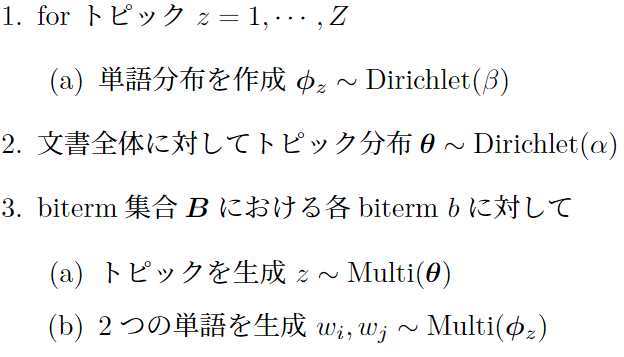
\includegraphics[width = 9cm]{images/BTM生成過程.png}}
    \caption{BTMの生成過程}
    \label{fig:BTM生成過程}
\end{figure}
\begin{figure}[ht]
    \centering
    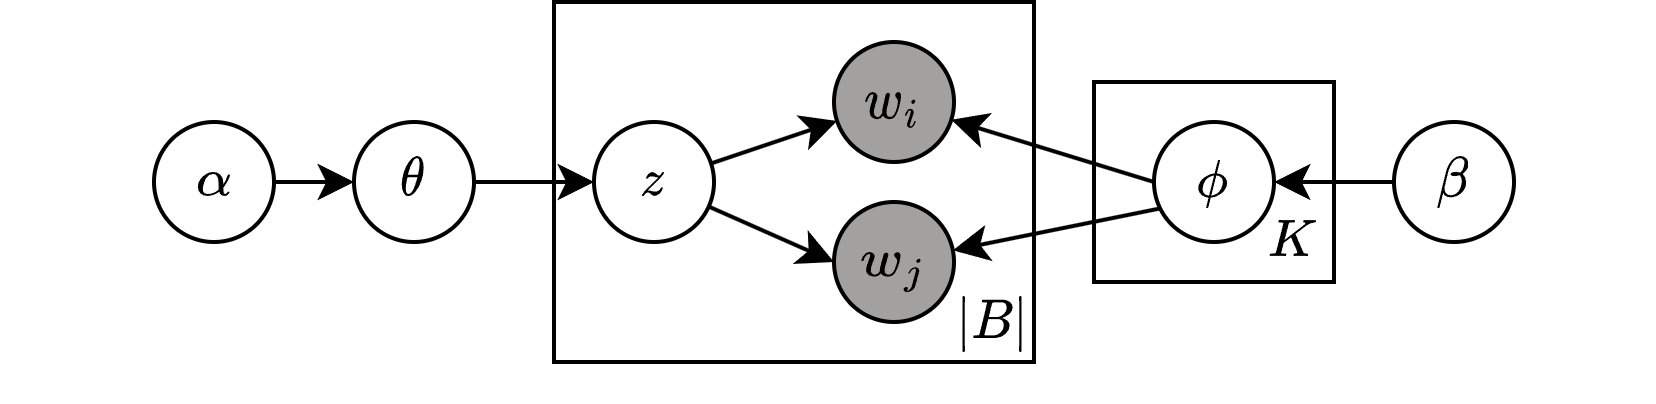
\includegraphics[width = 12cm]{images/BTMグラフィカルモデル.drawio.png}
    \caption{BTMのグラフィカルモデル}
    \label{fig:BTMのグラフィカルモデル}
\end{figure}
\newpage
まず, 各トピック$z$に対して単語分布$\boldsymbol{\phi}_z$がディリクレ分布に従って生成される. 
次に, 文書全体に対してトピック分布$\boldsymbol{\theta}$がディリクレ分布に従って生成される. 
LDAでは各文書に対してトピック分布が存在していたため, 短い文書や単語が少ない文書ではトピックを適切に
推定することが困難であるが, BTMでは文書全体で集約された単語の共起性を利用するためLDAに比べて優れたトピックの推定が行える.
そして, 各biterm $b$に対してトピック分布$\boldsymbol{\theta}$に従いトピック$z$が選択される. 
選択されたトピック$z$の単語分布$\boldsymbol{\phi}_z$から二つの単語を生成する. 
図\ref{fig:BTM生成過程}の手順に従ってbiterm $b = (w_i, w_j)$の同時確率は式(\ref{equation:BTM同時確率})のように, 
文書全体の尤度は式(\ref{equation:尤度})のように表せられる. \\
\begin{align}
    P(b) &= \sum_{z}P(z)P(w_i|z)P(w_j|z)\notag\\
         &= \sum_{z}\theta_z \phi_{i|z} \phi_{j|z}
    \label{equation:BTM同時確率}
\end{align}
\vspace{3truept}

\begin{equation}
    P(B) = \prod_{(i,j)}\sum_{z}\theta_z \phi_{i|z} \phi_{j|z}
    \label{equation:尤度}
\end{equation}
\vspace{5truept}

このようにBTMではbitermという二単語の対をモデル化の基本単位としているため, 
単語の数が少ないような短い文書でも文書集合全体の単語の共起性をとらえることでトピック推定の精度を向上させている. 
また, LDAとは異なり単一の文章を生成するという仮定ではなく, 文書集合から抽出したbitermを対象にそれらを生成するという仮定を持つ. 
つまり, 短い文書の場合にLDAでは少ない単語の情報から文書ごとのトピック分布を推定するのに対し, BTMでは全文書に出現する単語の共起
から文書集合全体のトピック分布を推定するため精度が高くなる. 
本研究で実験対象とするYouTubeの動画に対するコメントは比較的一文が短いものが多く, BTMの優位性が予測される. 
BTMを用いた具体的な提案手法は5.3節で述べる. 





\newpage
\section{提案手法}
ここでは, 前項で説明したBitem Topic Modelを用いて, YouTube上で自社製品やサービスを宣伝している動画
に対するユーザーのコメントから, 宣伝している商品やサービスに対して関連性が高いコメントを抽出する
システムを提案する. また, 提案したシステムの精度を検証する方法についても説明する. 
\subsection{データ収集}
実験に用いるYouTubeのコメントは, YouTube Data API v3を用いて取得した. YouTube Data API v3はGoogle Cloud Consoleで
APIキーを作成し, APIを有効化することで様々なYouTubeデータにアクセスすることが可能になる. 
そのうち, YouTubeのコメントに関連するものとして表\ref{table:データ収集}のようなデータが挙げられる. 
\begin{table}[h]
    \caption{YouTube Data API v3 で取得できるコメント情報}
    \vspace{5truept}

    \centering
    \begin{tabular}{ll}
        \hline
        項目 & 内容 \\
        \hline\hline
        videoID & コメントした動画のID\\
        textDisplay & 現在表示されているコメント\\
        textOriginal & 最初に投稿されているコメント\\
        authorDisplayName & コメント投稿者の名前\\
        authorProfileImageUrl & コメント投稿者のアイコン\\
        authorChannelUrl & コメント投稿者のチャンネル\\
        authorChannelId & コメント投稿者のチャンネルID\\
        likeCount & コメントに付いたいいねの数\\
        publishedAt & コメントの投稿日\\
        updatedAt & コメントの最終更新日\\
        \hline
    \end{tabular}
    \label{table:データ収集}
\end{table}

本研究では, 表\ref{table:データ収集}のうちtextDisplay(現在表示されているコメント)のみを抽出し, 実験を行なった. 
また, YouTubeのコメントには元のコメントの他に別のユーザーが返信しているケースも多いが, 本研究では返信しているコメントは扱わず, 
元のコメントのみを抽出し実験の対象としている. 抽出したコメントの一例を表\ref{table:元コメント}に示す. 
\vspace{10truept}

\begin{table}[h]
    \centering
    \caption{抽出したコメントの一例}
    \vspace{5truept}

    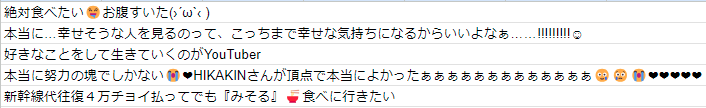
\includegraphics[width=14.5cm]{images/元コメント.png}
    \label{table:元コメント}
\end{table}
\newpage

\subsection{前処理手法}
トピックモデルを含む自然言語処理の様々な手法において, テキストデータに対する前処理は非常に重要である. 
Webテキストを扱う場合にはHTMLタグやJavaScriptのコードが含まれることもあり, 前処理としてそのような
ノイズを除去する必要がある. また, 本研究ではYouTubeの動画に対するコメントをテキストデータとして扱うが, 
YouTubeのコメントやSNSの投稿には絵文字や顔文字, URL, 話し言葉などを含んでいることが多い. 
そのため, 本研究でもトピックモデルによる分類を行う前の前処理は非常に重要である. 
本研究で行った主な前処理とその簡単な説明を以下に示す. 
\vspace{10truept}

\subsubsection{クリーニング処理}
\begin{description}
    \item[空白、改行文字を削除]\mbox{}\\
    半角空白や全角空白, 及び``\textbackslash n"などの改行文字を空文字に変換する.\\
    例:「おはよう 今日はいい天気ですね」→「おはよう今日はいい天気ですね」
    \item[記号除去]\mbox{}\\
    ``!''や``\#'', 及び全角記号を除去する. また, YouTubeのコメントの特性上顔文字が使われることも多い
    ため, それらを除去する目的でもある. \\
    例:「今晩、友達と映画を見に行く予定です!楽しみですね( ˇωˇ )」→「今晩友達と映画を見に行く予定です楽しみですね」
    \item[絵文字除去]\mbox{}\\
    顔文字と同様にYouTubeのコメントで使われることが多い. 感情分析などでは絵文字から情報を取得することもあるが, 
    本研究では感情に関する情報の抽出, 分析は行わないため絵文字は除去する. 
    \item[数字を0に置換]\mbox{}\\
    自然言語処理の様々な手法において, 数字は意味を為さないことが多いため, 
    1つ以上連続している数字を全て0に置換することが多い. 本研究でも数字に関する情報を必要としないため, 
    数字は全て0に置換する. \\
    例:「目標は年間で10回のイベントを開催することです」→「目標は年間で0回のイベントを開催することです」
    \item[単語の正規化]\mbox{}\\
    単語の正規化とは, 単語の文字種の統一, つづりや表記ゆれなどを無くすことである. この処理を行うことで
    同じ意味で異なる表記や形態の単語が同じ形になり, テキストの処理や解析が容易になる. 
    単語の正規化にはいくつか種類があり, 例えば
    \begin{itemize}
        \item テキスト内のアルファベットを全て小文字に変換する
        \item 半角カナを全角に統一する
        \item 辞書を用いた単語の統一
    \end{itemize}
    などがある. \\
    例:「Googleでネコの写真を検索してください」→「googleでネコの写真を検索してください」
    \newpage
    \item[連続長音記号除去, 繰り返し文字のまとめ]\mbox{}\\
    話し言葉や若者言葉でよくある「きたーーーーーー」や「うおおおおおお」など, 連続して長音記号が含まれている
    場合や同じ単語が繰り返されているものを削除, または一つにまとめる処理を行った. \\
    例:「食べたーーーーい!!」→「食べたーい」
    \item[その他の前処理]\mbox{}\\
    スパムの可能性があるため, URLを含むコメントを削除した. また, YouTubeの特性上外国人のコメントも多く存在したため, 
    日本語と英語以外の言語を含んでいるコメントを削除した. 
\end{description}

以上の前処理を表\ref{table:元コメント}のコメントに適用した結果を表\ref{table:前処理}に示す. 
\begin{table}[h]
    \centering
    \caption{前処理後のコメント}
    \vspace{5truept}

    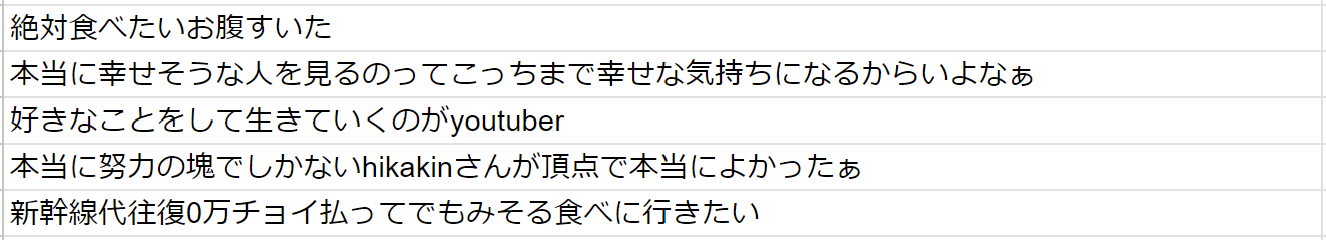
\includegraphics[width=14.5cm]{images/前処理適用.png}
    \label{table:前処理}
\end{table}

\subsubsection{MeCabによる形態素解析及び分かち書き}
次に, トピックモデルで学習する際に必要な文章の分かち書きを行う. 分かち書きとは, 自然言語処理の様々な手法において
文章を単語や形態素などの最小単位に分割する処理のことである. この処理を行うことで, 言語解析や機械学習の際に
テキストをより扱いやすい形態で実験を行うことができる. また, 英文の場合は単語間にスペースが明示的に存在するため
分かち書きは必要ない場合が多いが, 日本語に関しては単語間のスペースがなく, 文章を単語単位に分割する処理を
行わないと機械が単語を認識し解析することが難しくなるため, 分かち書きが必要である. 

本研究ではMeCabを利用して形態素解析, 及び分かち書きを行った. MeCabは京都大学情報学研究科と
日本電信電話株式会社コミュニケーション科学基礎研究所の共同研究で開発されたオープンソースの日本語形態素解析エンジンであり, 
日本語の文法や単語の品詞情報をもとに文章を形態素に分解したり, 品詞の付与などが可能である. 
本研究ではMeCabを利用して対象のコメントに対して形態素解析を行い, 形態素に分割後スペース区切りで繋ぐことで分かち書きを行う. 
MeCabには最初から分かち書きを行う機能も含まれているが, 形態素解析によって抽出した品詞をストップワード除去に用いるため
この手法で分かち書きを行う. 
   
また, 形態素解析の精度はエンジンのアルゴリズムの精度に加え, 形態素解析辞書の精度にも左右される. 
そのため, 形態素解析の目的にあった辞書を指定し, 解析することが重要となる. 表\ref{table:辞書比較}はMeCabで形態素解析を行うときに主に用いられている
辞書を比較したものである. 通常, MeCabでの形態素解析には標準搭載されているmecab-ipadicを用いるが, mecab-ipadicは基本的な文法や
専門用語に強い反面, 辞書の更新がないため新しい単語や固有表現に弱いという特徴がある. 
本研究の分析対象であるYouTubeの動画に対するコメントは比較的新しい言葉や固有名詞などを含むことが多いため, 
mecab-ipadicに多数のweb上の言語資源から得た新語を追加し, カスタマイズしたmecab-ipadic-NEologdを本研究では形態素解析の辞書に用いている. 
\begin{table}[ht]
    \caption{形態素解析辞書の比較}
    \vspace{5truept}

    \centering
    \begin{tabular}{cp{10cm}}
        \hline
        形態素解析辞書 & 特徴 \\
        \hline\hline
        mecab-ipadic & IPAコーパスをもとにしたMeCabに標準搭載されているIPA辞書. 基本的な日本語の文法や専門用語などの固有名詞に強いが, 辞書の更新がないため新しい言葉や固有名詞に弱い. \\
        \hline
        UniDic-mecab & 言語学・国語学や音声情報処理など, より多様な目的に適した辞書. 「短単位」という揺れが少ない斉一な単位を見出し語に採用している. \\
        \hline
        mecab-ipadic-NEologd & 多数のweb上の言語資源から得た新語を追加しカスタマイズしたMeCab用のシステム辞書. 辞書の更新が行われるので, 新しい固有表現に強い. \\
        \hline
    \end{tabular}
    \label{table:辞書比較}
\end{table}
\newpage

MeCabによる形態素解析, 及び分かち書きの処理を行った後, 2.2節で述べた通り品詞によるストップワード除去を行う. さらに一般的なストップワードリストを
用いたストップワード除去を組み合わせることで, 最終的に実験に用いるテキストの形式として整形する. 品詞によるストップワード除去では, 助詞・助動詞
などのトピック分類に必要ない品詞を除く手法や, 名詞・形容詞などのトピックにかかわる品詞を抽出する手法で行う. 
図\ref{fig:形態素解析}ではmecab-ipadicとmecab-ipadic-NEologdで形態素解析した結果を比較している. 例えば, 近年登場した少年漫画である「鬼滅の刃」という単語を含む文章を形態素解析した場合, 
mecab-ipadicでは``鬼'' ``滅'' ``の'' ``刃''と分割されてしまっているが, 辞書の更新が行われるmecab-ipadic-NEologdでは
``鬼滅の刃''と一単語で認識されていて, 適切な形態素解析が行われていると言える. 
\vspace{10truept}

\begin{figure}[h]
    \centering
    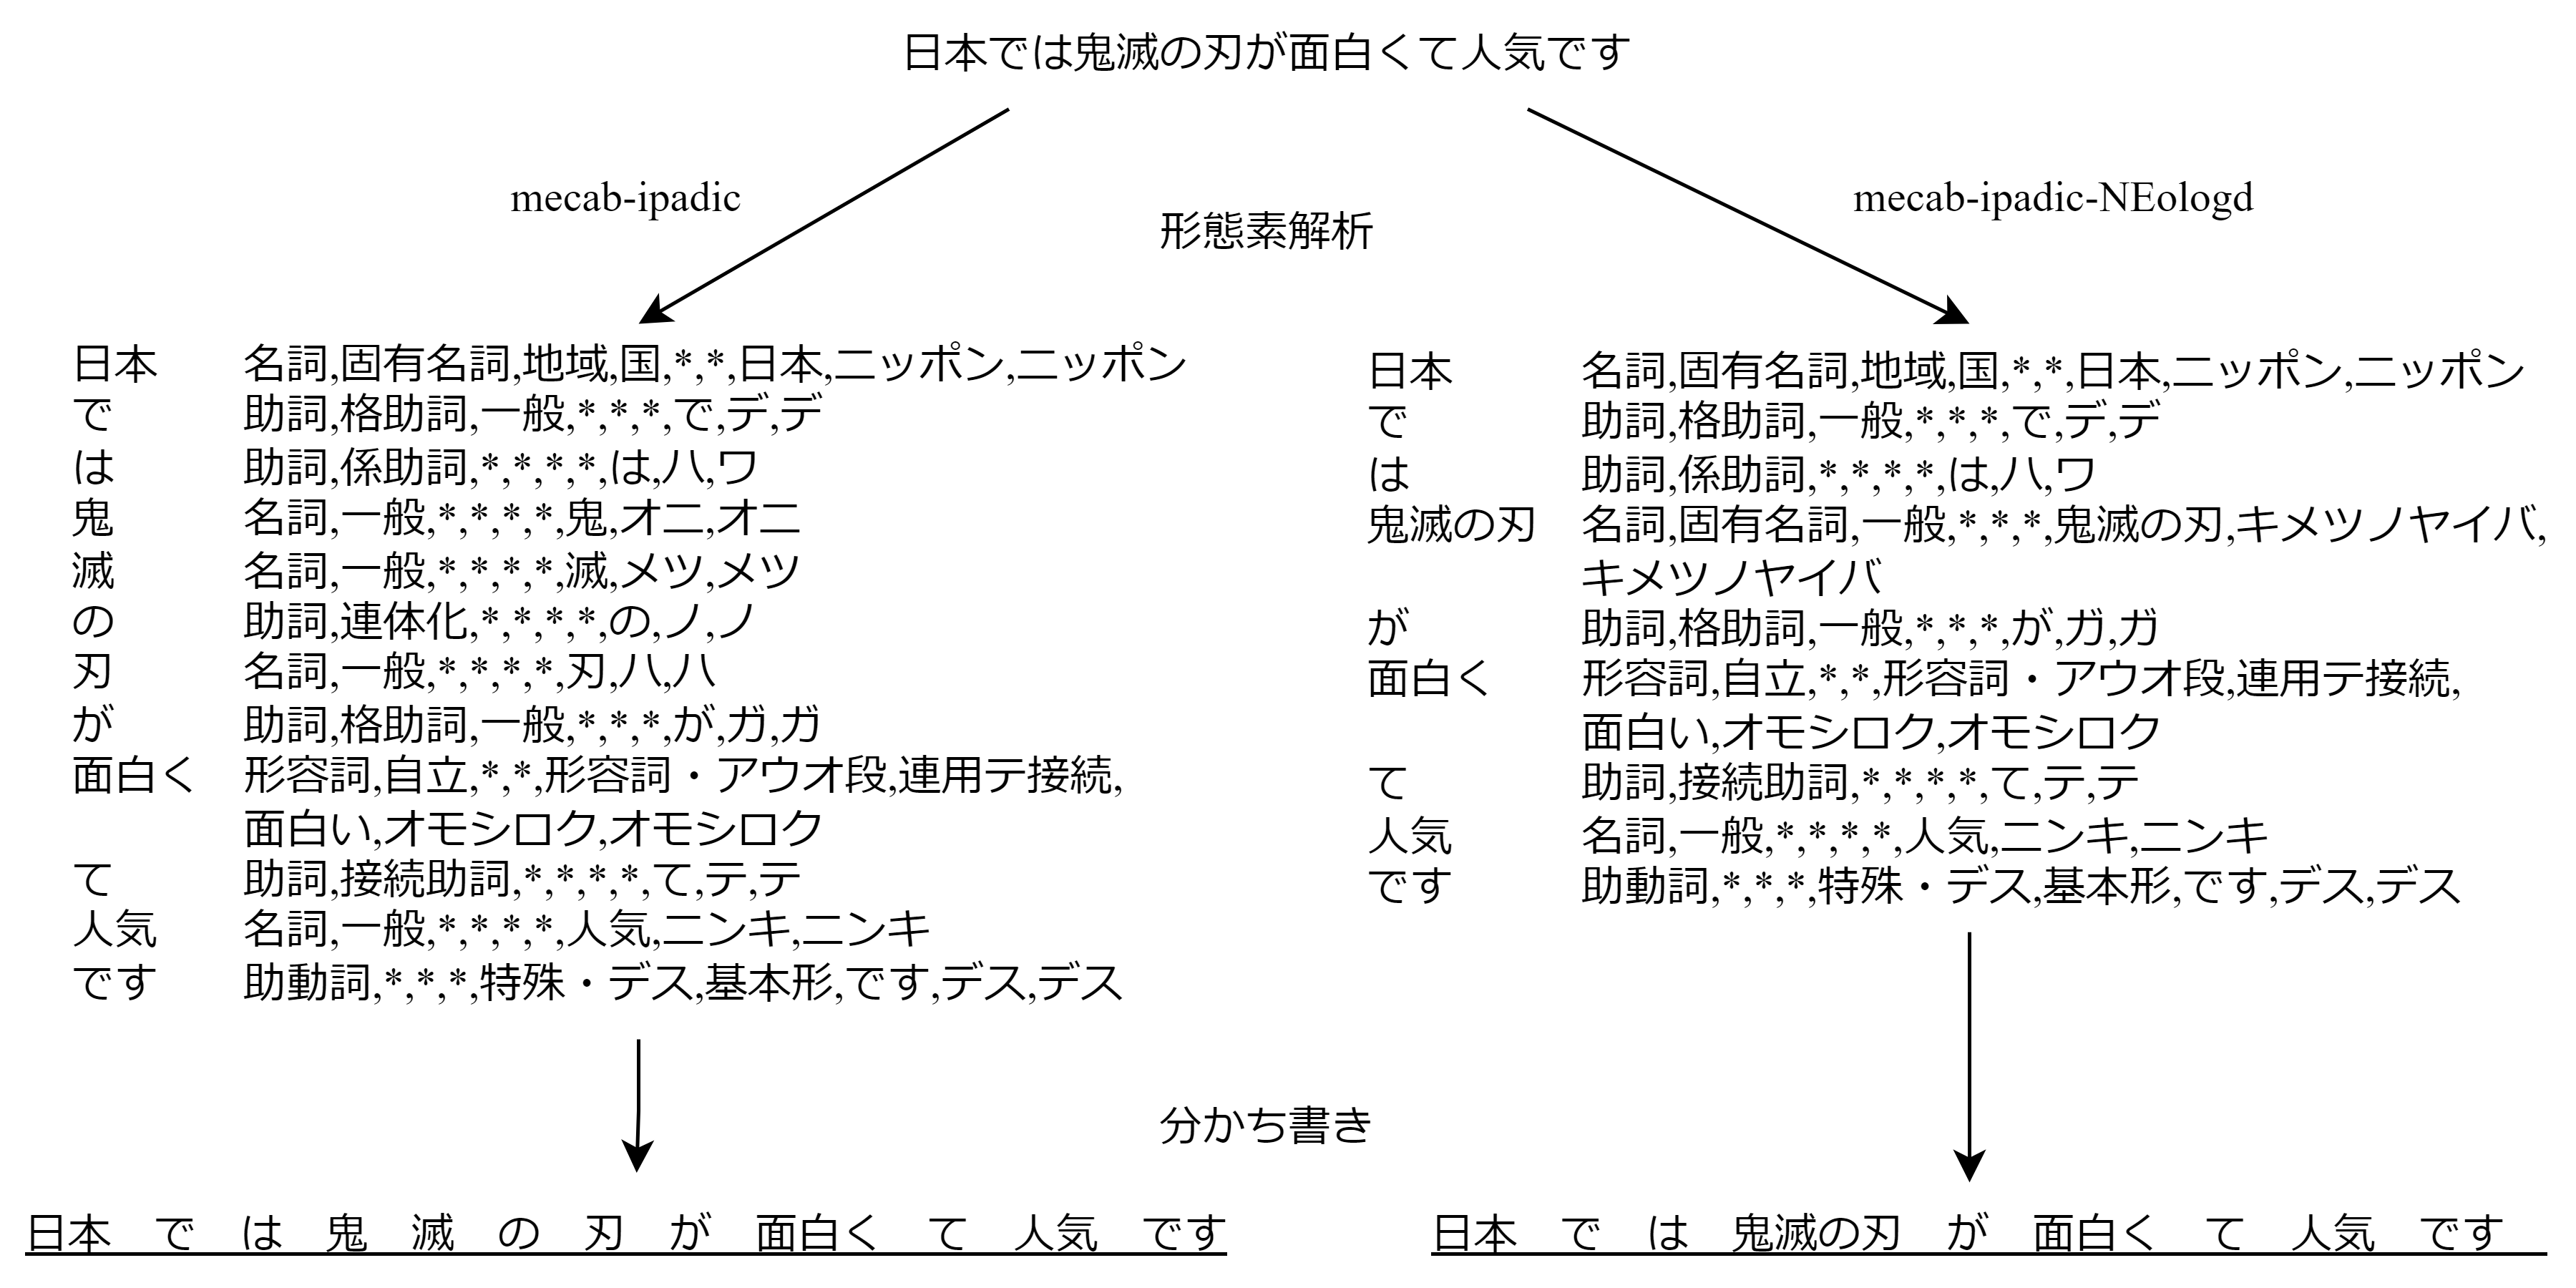
\includegraphics[width = 14.6cm]{images/形態素解析.drawio.png}
    \caption{辞書による形態素解析結果の比較}
    \label{fig:形態素解析}
\end{figure}

\newpage
\subsection{BTMによるトピック抽出}
前処理及び分かち書きを行ったテキストデータに対して, 4.2節で説明したBiterm Topic \\
Model(BTM)を用いてトピックの推定, 及び単語分布の推定を行う. 
BTMの実装にはPythonのライブラリであるbitermplusを用いた. 
bitermplusのget\_words\_freqs()メソッドを用いて, 
整形したテキストデータから全ての単語リスト, 及び各単語の頻度などを抽出する. 
抽出した単語リストを基に, get\_vectorized\_docs()メソッドを用いて与えられたテキストデータ内の各文書をベクトル形式に変換する. 
ベクトル化した各文書から隣接する単語の対(biterm)をget\_biterms()メソッドを用いて生成する. 
ここで生成したbitermにより文書内の単語の共起性の情報を捉え, トピックをより正確に推定することができる. 
生成したbitermを用いてBTMを訓練し, トピック分布, 及び単語分布を生成する. 
モデルを訓練する際にはいくつかのパラメータが存在し, 生成するトピック数:$T$, 各文書で考慮する単語数:$M$, ディリクレ分布のハイパーパラメータ
$\alpha, \beta$などが重要なパラメータである. 
本研究では一つの動画に対するコメント集合に対してBTMを用いるため, トピック数$T$はあまり大きくなくかつ最低限複数のトピックを
抽出できるように$T=5$とした. 
各文書で考慮する単語数とは, モデルの学習に使用する各文書の単語数を示しており, 各文書中の頻度上位$M$個の単語をトピックモデル
の学習に用いる. 本研究の実験対象は一文が比較的短い文章であり含まれる単語数も少ないため$M=10$とした. 
トピック分布, 及び単語分布を生成するディリクレ分布のハイパーパラメータ$\alpha, \beta$は本研究ではスカラー値
を採用しており, その値は対象とする動画によって最適な値を求めて実験を行う. 
以上の手順通りBTMを学習し, 推定した各トピックごとの単語分布より, 出現確率上位$n$単語を抽出する. 
$n$は後述する文章生成の際に冗長な文とならないような値を選択する必要があり, 本研究では$n=10$を基本的な値とした. 
図\ref{fig:BTM出力例}にBTMによって抽出したトピック($T=5$)とその出現確率上位10単語の例を示す. 
これは新作のカップラーメンを紹介している動画に対するコメントであり, 図\ref{fig:BTM出力例}の結果にあるように
「ラーメン」や「味噌ラーメン」, 商品開発者である「ヒカキン」などの単語が抽出できていることが分かる. 
また, 図下部にあるperplexityはトピックモデルの性能評価によく使われている指標である. 
perplexityはモデルに従って単語を選ぶ困難さを表していて, 
各単語の出現確率の逆数の幾何平均で定義されている(式(\ref{equation:perplexity})).
直感的にはperplexityはモデルによって生成する単語の候補数に対応していて, 候補数が少ない方が正解となる単語を当てやすいため,  
perplexityは低い方がモデルとしての性能が高いことを示している. 
本研究ではこのperplexityをモデルの性能評価に用いてハイパーパラメータ$\alpha, \beta$を調整する. \\
\vspace{5truept}

\begin{equation}
    \textrm{perplexity(\bm{W}|M)} = exp\left(-\frac{\sum_{d=1}^{D}\log p(\bm{w}_d|M)}{\sum_{d=1}^{D}N_d}\right)
    \label{equation:perplexity}
\end{equation}
\vspace{30truept}

\begin{figure}[h]
    \centering
    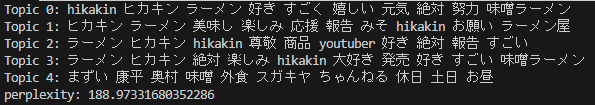
\includegraphics[width = 14.6cm]{images/BTM出力例.png}
    \caption{BTMの出力例}
    \label{fig:BTM出力例}
\end{figure}

\newpage
\subsection{文章生成}
各トピックごとの出現確率上位の単語を抽出した結果を用いて, 各トピックごとに文章を自動で生成する. 
抽出した単語は各トピックの出現確率上位の単語であるため, ここで生成された文章は各トピックごとに
代表的であるという仮説を立て, 以降の手法に適用する. 
文章を自動で生成する方法として, 大規模言語モデルであるGPT-4を搭載したChatGPTを用いる方法で行った. 
プロンプトには以下のルールを入力して各トピックごとに文章を生成した. 
\begin{description}
    \item[抽出した単語を空白区切りで入力する]\mbox{}\\
    BTMによって抽出した$n$単語($n$は抽出する単語数)を空白区切りで入力する. ChatGPTに正しく単語を認識させるため, 
    空白区切りにする必要がある. 
    \item[全ての単語を使用する] \mbox{}\\
    抽出した単語を全て使用することで, 後述する類似度計算の精度を向上させる.  
    \item[人名がある場合は指定する]\mbox{}\\
    人名をChatGPTが認識できない場合, 文章が支離滅裂になる可能性があるため個別に指定する. 
    \item[一つの文章に多くの単語を用いて, 文章数は少なくする]\mbox{}\\  
    生成される文章はトピックごとに代表的であるという仮説の元, YouTubeのコメントの特徴に近い
    文章を生成したいため, 長文を避けるようなルールを追加している. 
    \item[YouTubeのコメントのように生成する]\mbox{}\\
    人が投稿するコメントに近しい文章を生成する. 
\end{description}
\vspace{20truept}

図\ref{fig:文章生成}にChatGPTに入力する単語, プロンプト, 出力結果の例を示す. 提案手法では各トピックごとに
文章を生成するため, 図\ref{fig:文章生成}のような結果がトピックの数だけ生成される. 
\begin{figure}[h]
    \centering
    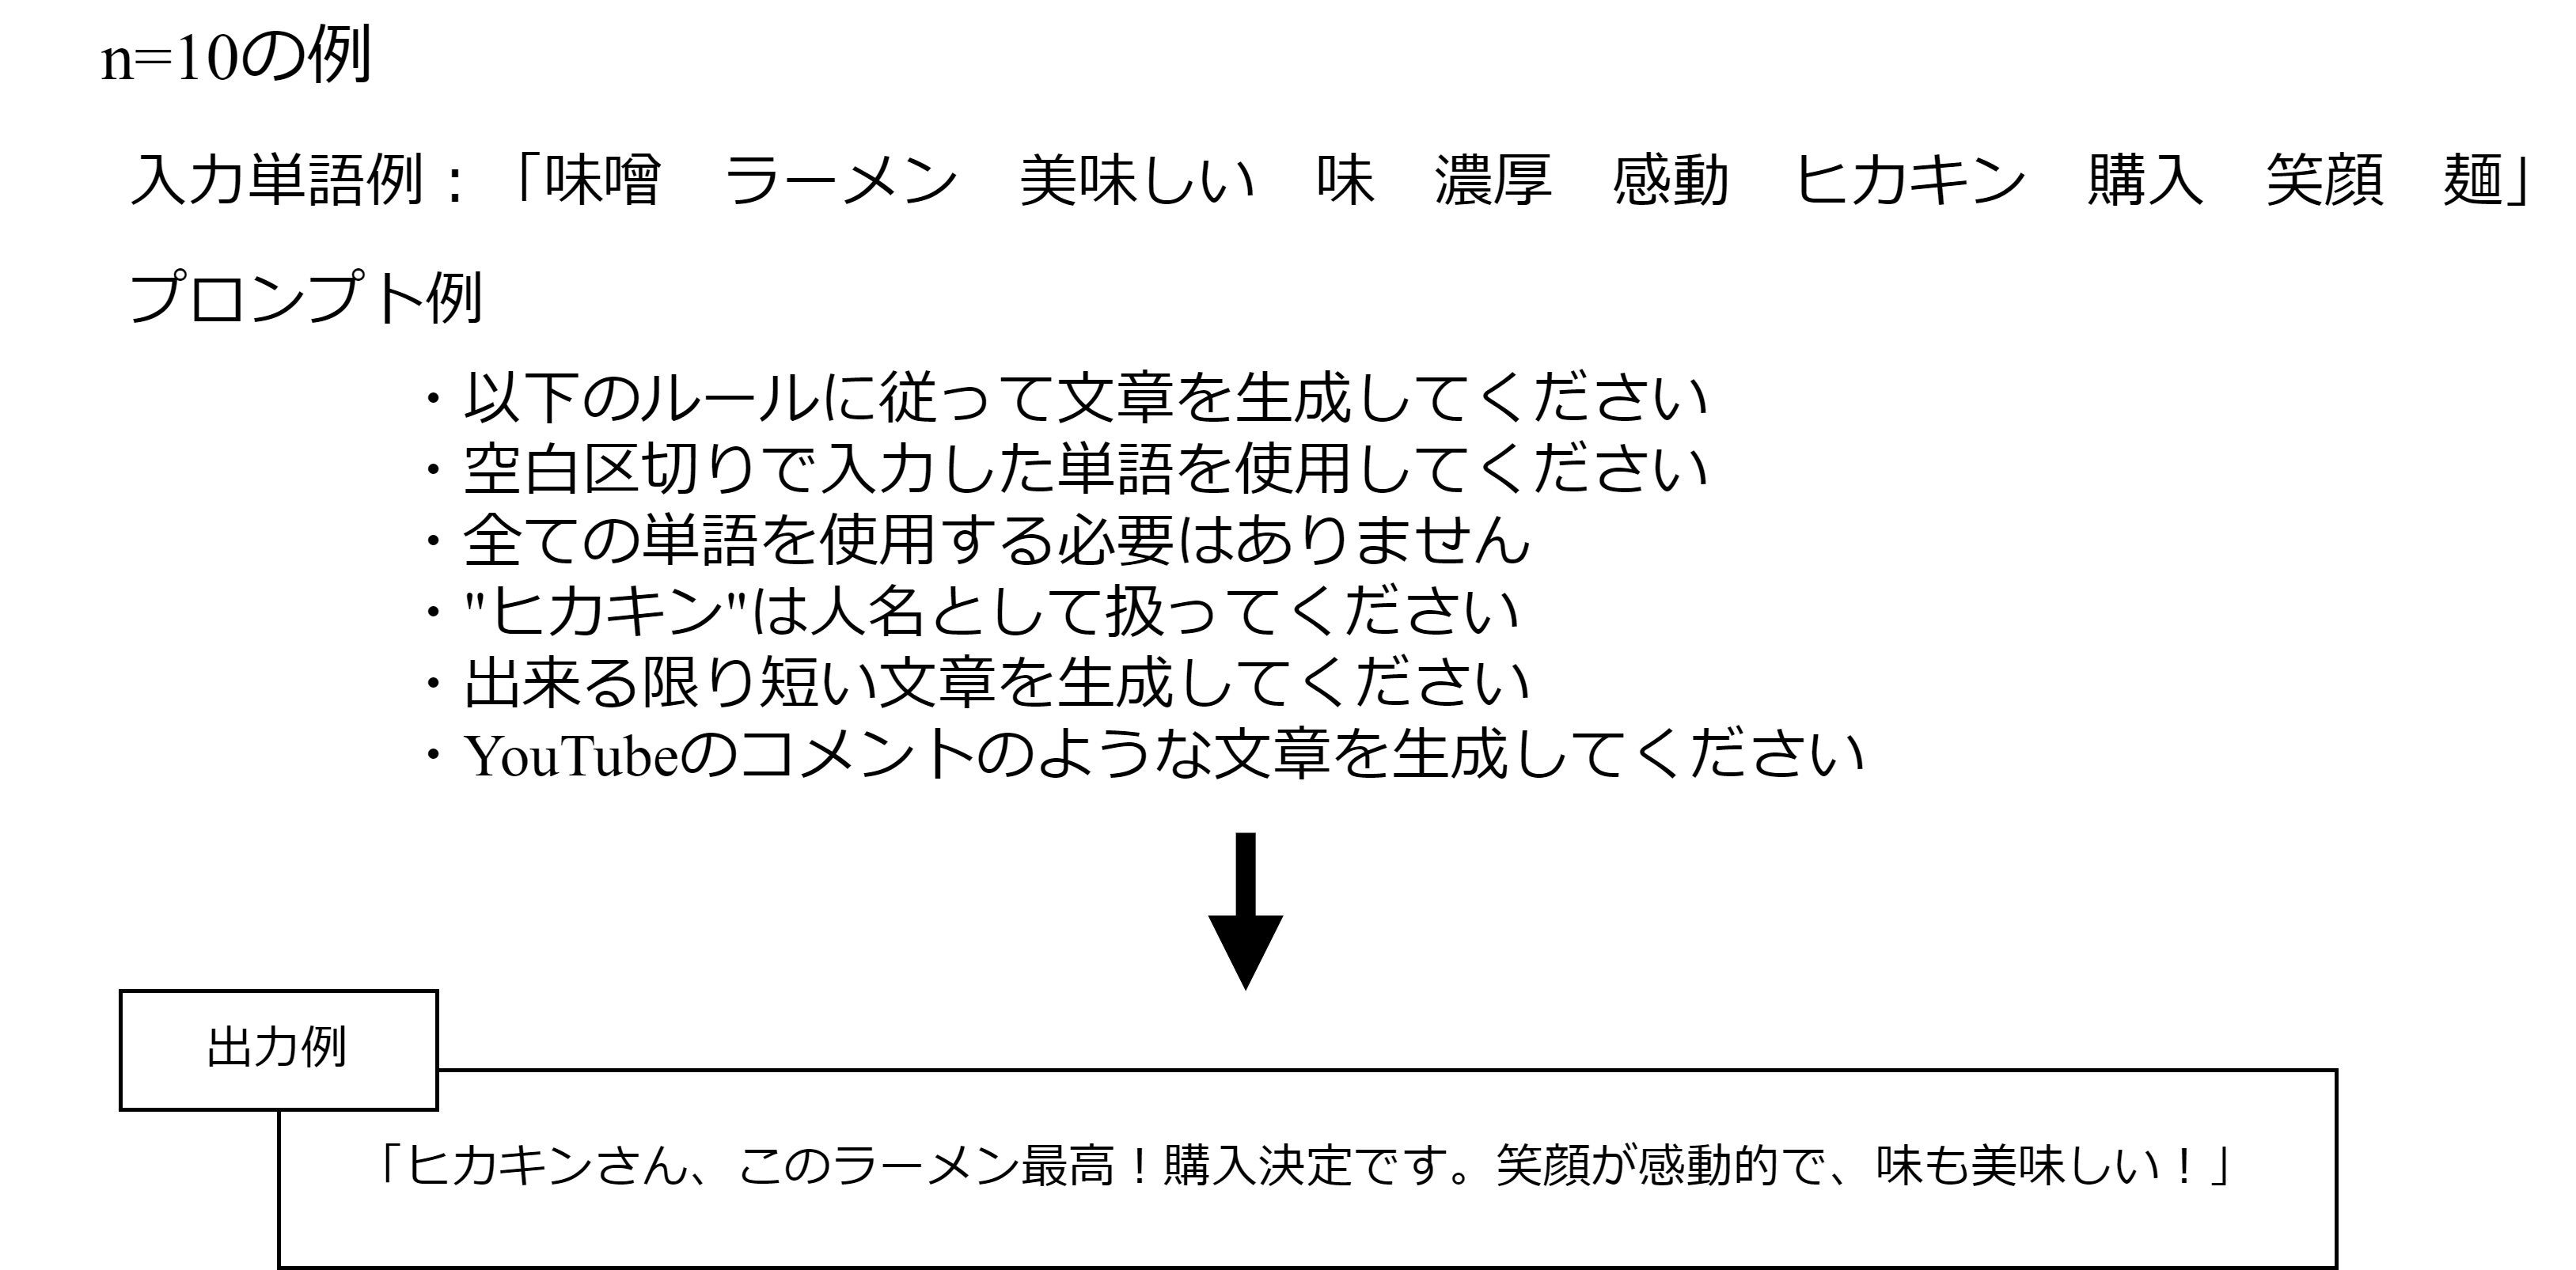
\includegraphics[width = 14.6cm]{images/文章生成.drawio.png}
    \caption{ChatGPTを用いた文章生成例}
    \label{fig:文章生成}
\end{figure}

\newpage
\subsection{文章間の類似度計算}
前節でChatGPTを用いて自動で生成した文章と, 5.2.1節で述べたクリーニング処理を施した
YouTubeの元コメントとの文章間の類似度を計算し, 数値が高い順に並び替えることで, 本研究の目的である, 
YouTube上で自社製品やサービスを宣伝している動画に対するコメントのうち
他のユーザーがその商品の購入を検討する際に参考にできるようなコメントの抽出を実現する. 
文章間の類似度計算手法にはCos類似度を用いる. Cos類似度とは, 二つのベクトルが「どれくらい似ているか」
を表す尺度であり, 二つのベクトルがなす角のCos値のことである. Cos類似度は, 式(\ref{equation:Cos類似度})のように二つのベクトルの内積
を二つのベクトルのノルムで割ることで求められる. 
\vspace{5truept}

\begin{equation}
    \textrm{Cosine\ Similarity} = \dfrac{\boldsymbol{A}\cdot \boldsymbol{B}}{\|\boldsymbol{A}\|\,\|\boldsymbol{B}\|}
    \label{equation:Cos類似度}
\end{equation}
\vspace{5truept}

前節で生成した文章は, 元のコメント集合から抽出した潜在的なトピックごとの代表的な文章である
という仮説を立てていることから, 生成した文章との文章間のCos類似度が高いYouTubeの元コメントは
そのトピックとの関連性が高い文章といえる. また, 本研究では抽出したトピックにラベル付けを行わないため, 
どのようなトピックとの関連性が高いかは判断することができない. しかし本節で行う類似度計算では
生成したトピック数の文章全て($k$=5であれば5文全て)と元のコメント一文とのCos類似度をそれぞれ計算し, 
一番高い数値をその文章の類似度として扱うため, 具体的に何に関するトピックかは判断できないが
動画内容との関連性を数値で示すことができると考えた. 

Cos類似度は二つのベクトルの類似度を計算するため, 本手法に用いる上で文章をベクトル化する必要がある. 
文章をベクトル化する手法は数多く存在するため, 目的によって適切な手法を選択することが重要である. 
本研究では, 単語の重要度を考慮できるTF-IDFによる文章のベクトル化と, 
様々なタスクに適応できる汎用性を持つBERTの事前学習済みモデルを用いた文章の埋め込み(ベクトル化)
の二つの手法で実験を行う. 
\subsubsection{TF-IDF}
TF-IDFとは, Term Frequency(単語頻度)とInverse Document Frequency(逆文書頻度)の積で定義される, 
文書中のある単語の重要度を表す指標である. TFは「一つの文書$d$に単語$t$がどれだけの割合で出現したか」を定量的に
表した指標であり, 式(\ref{equation:TF})で表せられる. ここで, $n_{d,t}$は文書$d$中に単語$t$が出現する回数, $T$は一つの文書における単語数の合計である. 
\vspace{5truept}

\begin{equation}
    TF_{d,t} = \dfrac{n_{d,t}}{\sum_{t=1}^T n_{d,t}}
    \label{equation:TF}
\end{equation}
\vspace{5truept}

IDFは「ある単語を含む文書が文書集合の中でどれくらいの割合を占めているか」を定量的に表した指標であり, 
実際の式(\ref{equation:IDF})ではその割合の逆数の対数を取っている. つまり, 「ある単語が一部の文書にしか現れない度合い」を計算していることとなる. 
ここで, Nは全体の文書数, $df_t$は単語$t$が出現する文書数を表す. 
\vspace{5truept}

\begin{equation}
    IDF_t = \log\dfrac{N}{df_t}
    \label{equation:IDF}
\end{equation}
\vspace{5truept}

\newpage
\noindent
TF-IDFは式(\ref{equation:TF-IDF})のようにTF(式(\ref{equation:TF}))とIDF(式(\ref{equation:IDF}))の積で表せられる. 
\vspace{5truept}

\begin{equation}
    TF\mathchar`-IDF_{d,t} = TF_{d,t}\times IDF_t
    \label{equation:TF-IDF}
\end{equation}
\vspace{5truept}

\noindent
したがって, TF-IDFは以下の条件のときに高い数値を示す. 
\vspace{5truept}

\begin{itemize}
    \item その単語の単語頻度が高い
    \item 文書集合全体に対して, その単語の文書頻度が低い
\end{itemize}
\vspace{5truept}

\noindent
この計算を全ての文書, 単語に対して行うことで文書に含まれる単語の重要度から文書の特徴を定量的に
求めることができる. そして, 各単語に対するTF-IDF値を要素としたベクトルを生成し, Cos類似度の計算に用いる. 

\subsubsection{BERT}
BERT(Bidirectional Encoder Representations from Transformers)はGoogleによって2018年に開発された
Transformerをベースとした自然言語処理モデルである. 従来の自然言語処理モデルでは文章を前から読み文脈を理解していくのに対して, 
BERTではMasked Language Model(MLM)というモデルを使用することで文章を文頭と文末の双方向から学習している. 
MLMではテキストの一部を[MASK]という別の単語で置き換えたテキストを入力し, その前後の文脈に基づいて[MASK]の単語を予測
するようにモデルを訓練する. 文章を双方向から学習することにより, ある単語の前後の文脈を捉えることができ自然言語処理
モデルとしての性能を大幅に向上させた. 加えて, 文単位での学習を行うNext Sentence Prediction(NSP)という手法を組み合わせることで
さらにモデルの性能を向上させている. NSPは二つの文章の関係性について予測するタスクであり, 二つの文章を入力した後に
「二つの文章は連続しているかどうか」を判定するタスクを繰り返すことで学習を行う. 図に示すように, 二つの文章が連続している場合はIsNext
, そうでない場合はNotNextの判定を行う. 各入力の最初にある[CLS]トークンは主に分類タスクにおいて使用され, [CLS]
トークンに関連付けられた隠れ層の状態(ベクトル)が入力文の全体的な意味を捉えるようになる. また, [SEP]は文の区切りを示している. 
このNSPという手法により, 単語だけではなく文章のつながりに関して学習することができる. 
\vspace{10truept}

\begin{figure}[ht]
    \centering
    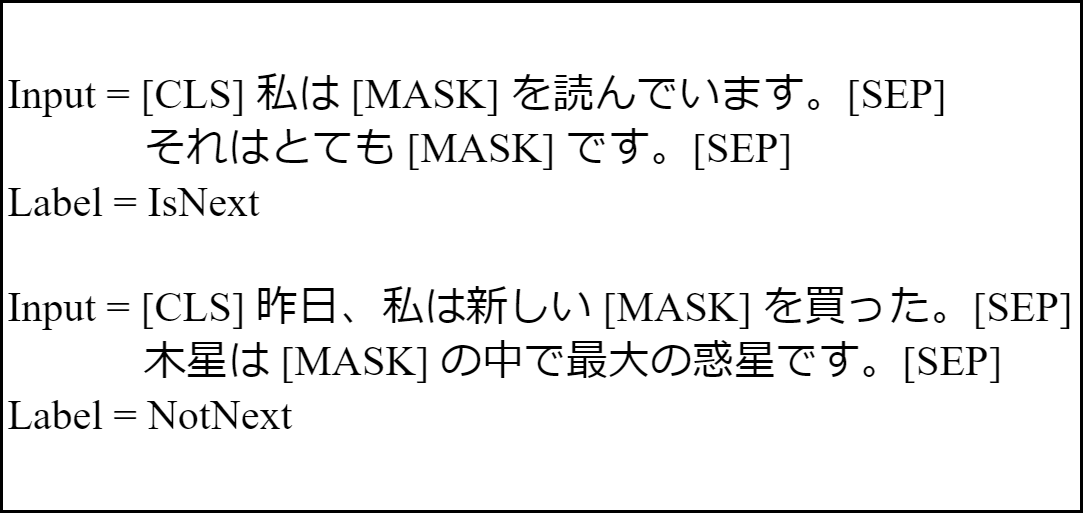
\includegraphics[width=10cm]{images/BERT.drawio.png}
    \caption{NSPによる文章のつながり判定例}
    \label{fig:BERT}
\end{figure}
\newpage

本研究では, このBERTモデルを用いた文章の埋め込み(ベクトル化)を行い, Cos類似度の計算に用いている. 
BERTモデルでは, テキストを前処理した後トークン化する. BERTにおけるトークン化は通常の単語分割よりも複雑な場合があり, 
例えば単語本体と接頭辞, 接尾辞に分割するサブワード分割を行うことがある(例:``playing''→[``play'', ``\#\#ing'']). 
また, BERTの出力は入力された各トークンに対する文脈依存の埋め込みである. これらの埋め込みは単語の意味がその文脈によって
どのように変化するかを捉えることができる. 例えば, 「この部屋は明るい」と「彼は明るい性格だ」では「明るい」の意味が異なり, 
文章埋め込みの出力結果も異なる. 
このようにBERTモデルを使用した文章の埋め込みでは, 文章を双方向から学習することで文脈の理解において高い精度を示したり, 
単語の意味の差異を理解し適切な結果を出力したりできる. 
このBERTモデルを使用した文章のベクトル化と, 先述したTF-IDFを用いた手法とを比較して実験を行い, 本研究の目的に対してより効果的な
手法がどちらなのかを検証する. 
\vspace{30truept}

\subsection{提案手法の精度検証}
前節までの提案手法によるシステムの妥当性, 及び精度を検証するため, 人手で評価したデータとの比較を行う. 
人手による評価として, 5.2.1節で述べたクリーニング処理を施した元のコメント文に対して, 
動画で宣伝している商品やサービスに関連しているかどうかを人手でアノテーションし, ラベル付けを行う. 
アノテーションの基準として以下のようなルールに当てはまるコメントに「関連性-高」のラベルを付け, その他のコメントに
「関連性-低」のラベルを付与し, 正解ラベルが付いたデータを作成する. 
\vspace{10truept}

\begin{itemize}
    \item 動画で宣伝している商品やサービスに直接関係している
    \item 商品やサービスに対する視聴者の意見・感情などを含んでいる
    \item 商品やサービスを宣伝している動画内容に関係している
\end{itemize}
\vspace{10truept}


「関連性-高 / 低」の二値分類を行った結果から, 「関連性-高」ラベルを付けたコメントの件数をa, 「関連性-低」
ラベルを付けたコメントの件数をbとする. 
そして, 前節で文章間の類似度を計算し降順にソートしたテキストデータの上位a件を「関連性-高」と予測したデータ, 
下位b件を「関連性-低」と予測したデータとみなし, 正解ラベルを付与したデータと予測データに対してConfusion Matrix(混同行列)
を求める. Confusion Matrixとは, 二値分類問題で出力された結果をまとめた行列(≒表)のことで, 機械学習モデルの性能を測る指標として
用いられていることが多い. 本研究では, 「関連性-高 / 低」の二値分類に関して, 提案手法により予測したデータを機械学習モデルで予測したデータ
とみなし, Confusion Matrixを求める. 

表\ref{table:Confusion Matrix}が一般的な機械学習モデルにおけるConfusion Matrixである. 行が正解のクラス(ラベル)を, 列が機械学習モデルで予測したクラス(ラベル)を表している. 
TP(True Positive)はPositiveラベルが付いているものを正しく「Positive」だと予測していて, 注目対象を正しく分類できる, また対処すべき注目事象を特定できることを表す. 
TN(True Negative)はNegativeラベルが付いているものを正しく「Negative」だと予測していて, 注目対象以外を正しく分類できる, また注目対象を見逃さず損失を避けられることを表す. 
FN(False Negative)はPositiveラベルが付いているものを誤って「Negative」だと予測していて, 注目対象を誤ってそれ以外に分類してしまう, また注目対象を見逃し利益の獲得を逃してしまうことを表す. 
FP(False Positive)はNegativeラベルが付いているものを誤って「Positive」だと予測していて, 注目すべきではないものを誤って分類してしまう, また分類する事象によっては無駄なコストがかかることを表す. 
これらを使い, 機械学習モデルの性能を測る様々な指標を計算することができる. 
\vspace{10truept}

\begin{table}[h]
    \centering
    \caption{Confusion Matrix}
    \vspace{5truept}

    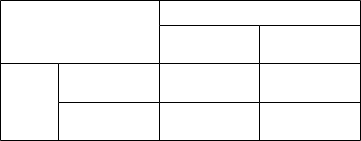
\includegraphics[width = 12cm]{images/Confusion_Matrix.drawio.png}
    \label{table:Confusion Matrix}
\end{table}
\vspace{5truept}

\noindent
以下に表\ref{table:Confusion Matrix}のConfusion Matrixの例から求められる様々な指標を示す. 
\vspace{10truept}

\begin{description}
    \item[Accuracy]\mbox{}\\
    正解率・正確度・精度などと呼ばれる, 全予測結果の中で正しい予測をしたもの(TP・TN)の割合のことである. 総合的なモデルの性能を示すのに用いられることが多いが, 
    クラスに偏りがある場合(例:Positiveが極端に多く, Negativeが極端に少ない), はモデルの性能を正しく評価できないこともある. \\
    \begin{equation}
        \textrm{Accuracy} = \dfrac{TP+TN}{TP+FP+FN+TN}
        \label{equation:Accuracy}
    \end{equation}
    \vspace{5truept}

    \item[Error Rate] \mbox{}\\
    不正解率と呼ばれる, Accuracyの逆で全予測結果の中で誤った予測をしたもの(FP・FN)の割合のことである.
    Accuracyと同様に, クラスの偏りがある場合にはモデルの性能を正しく評価できないこともある. \\
    \begin{equation}
        \textrm{Error Rate} = \dfrac{FP+FN}{TP+FP+FN+TN}
        \label{equation:Error}
    \end{equation}
    \vspace{5truept}

    \item[Sensitivity・Recall]\mbox{}\\
    感度・再現率・検出率などと呼ばれる, 正解クラスがPositiveであるとき, 予測モデルもPositiveだと判定した割合のことである. 
    実際に正解クラス(例:癌の検出など)を見逃さないことが重要な事象の際に重視される指標である. \\
    \begin{equation}
        \textrm{Sensitivity・Recall} = \dfrac{TP}{TP+FN}
        \label{equation:Recall}
    \end{equation}
    \vspace{5truept}

    \item[Specificity]\mbox{}\\  
    特異度と呼ばれる, 正解がNegativeであるとき, 予測モデルもNegativeだと判定した割合のことである. 
    疫病検査の例では, 罹患していない人の結果が陰性となる率であり, 負のケースを正確に識別することが重要な事象の際に重視される. \\
    \begin{equation}
        \textrm{Specificity} = \dfrac{TN}{FP+TN}
        \label{equation:Specificity}
    \end{equation}
    \vspace{5truept}

    \item[Precision]\mbox{}\\
    適合率と呼ばれる, モデルがPositiveと予測したときに実際にそれがPositiveである割合のことである. 
    偽陽性(誤った正の予測)を最小限に抑えたい事象のときに重視される指標である. \\
    \begin{equation}
        \textrm{Precision} = \dfrac{TP}{TP+FP}
        \label{equation:Precision}
    \end{equation}
    \vspace{5truept}

    \item[F1-measure]\mbox{}\\
    F1値・F値などと呼ばれる, Precision(適合率)とRecall(再現率)の調和平均のことである. 
    一般的にPrecisionとRecallの間にはトレードオフの関係があるが, そのバランスを取る必要がある事象のときに重視される指標である. \\
    \begin{equation}
        \textrm{F1-measure} = \dfrac{2\times \textrm{Precision}\times \textrm{Recall}}{\textrm{Precision}+\textrm{Recall}} = \dfrac{2\times TP}{2\times TP+FP+FN}
        \label{equation:F1}
    \end{equation}
    \vspace{5truept}

\end{description}

このようにConfusion Matrixを使用した機械学習モデルの性能評価には様々な指標が存在するが, 
どの指標がそのモデル・目的に対して最適な性能評価を行えるかの判断を行う必要がある. 
したがって, ここからは本研究の目的・提案手法においてどの指標が適切なのかを考えていく. 
表\ref{table:提案手法のconfusion}は本研究におけるConfusion Matrixを示している. 

Accuracy(正解率)は, 全予測結果の中で関連性があるコメント及び関連性がないコメントをどれだけ正確に分類できているかの指標である. 
関連性あり・なしのそれぞれのコメント数は動画内容・商品(サービス)・視聴者層などによって大幅に異なるため, 
偏りが発生しやすいと考えられる. 
\vspace{3truept}

\begin{table}[ht]
    \centering
    \caption{提案手法のConfusion Matrix}
    \vspace{5truept}

    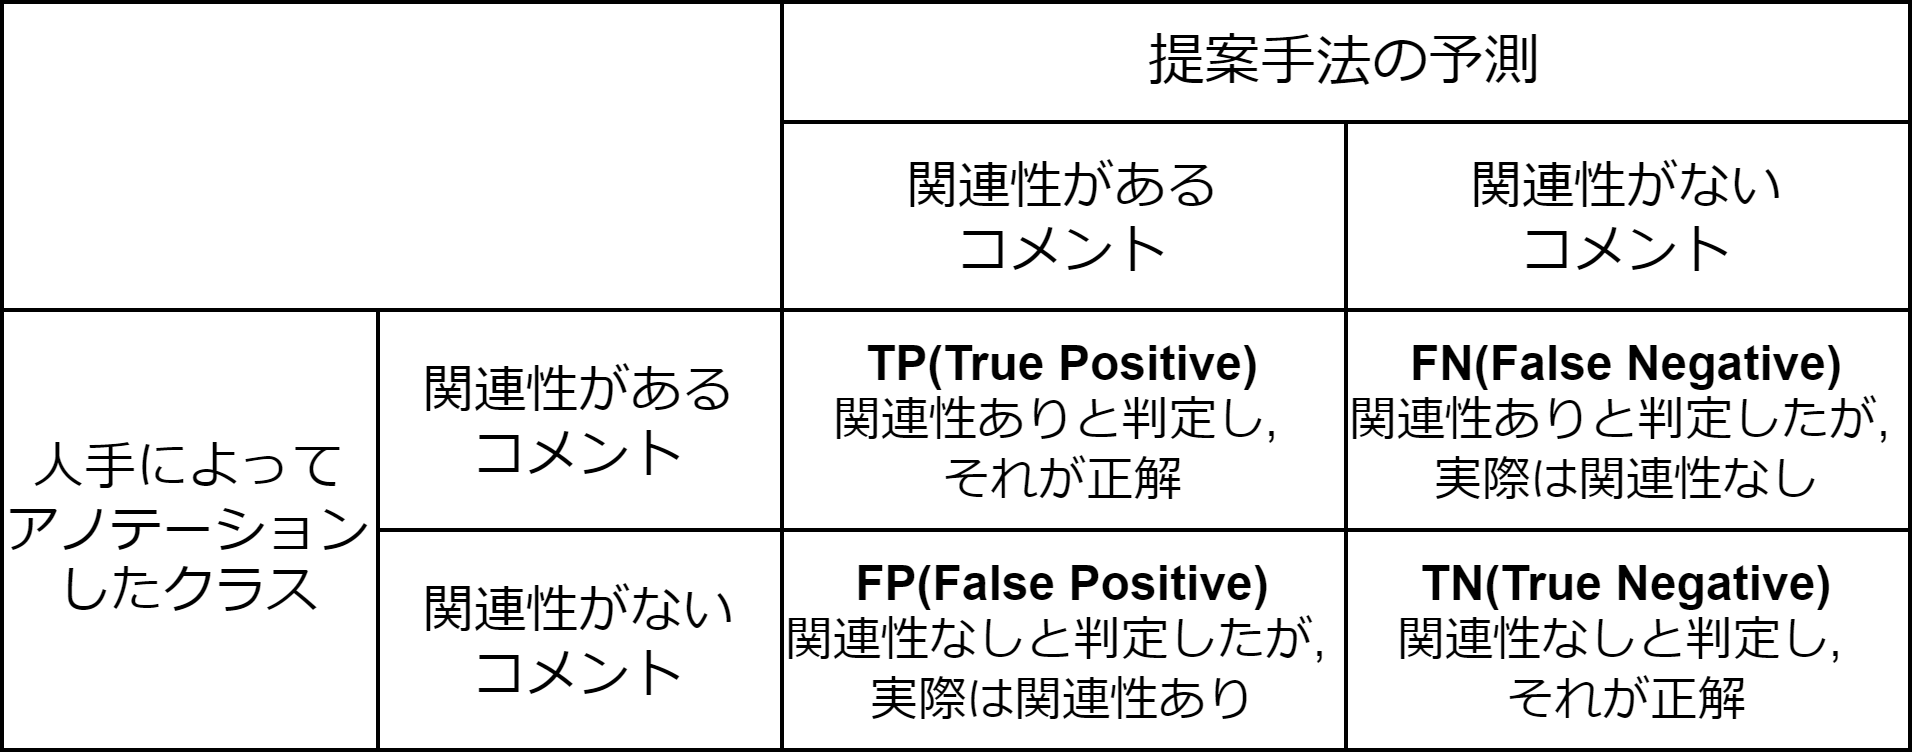
\includegraphics[width = 12cm]{images/提案手法のconfusion.drawio.png}
    \label{table:提案手法のconfusion}
\end{table}
\vspace{5truept}

\newpage
\noindent
つまり, Accuracyが高い場合でも, 特定の動画においてモデルが適切に性能を評価しているとは限らないといえる. 
Error RateはAccuracyと同様にクラスの偏り次第では適切な評価が行えない場合がある. 
Sensitivity・Recall(感度・再現率)は人手で関連性があると判断したコメントのうち, 提案手法によって関連性があると予測されたコメントの割合である. 
この値が高いということは, 実際に関連性があるコメントの取りこぼしが少ないことを意味しているので, 本研究の提案手法を評価する指標
として有効であると考えられる. 
Specificity(特異度)はSensitivity・Recallの逆で, 人手で関連性がないと判断したコメントのうち, 提案手法によって関連性がないと
予測されたコメントの割合である. 
本研究では商品・サービスとの関連性があるコメントを抽出する手法を提案しているため, Specificityは提案手法の評価をする指標として
適切ではないと考えられる. 
Precision(適合率)は提案手法によって関連性があると予測されたコメントのうち, 人手で関連性があると判断したコメントの割合である. 
この値が高いということは, 提案手法によって抽出したコメントを他のユーザーが確認したとき, それが実際に商品との関連性があり, 
商品を購入する際に参考になりうるコメントである可能性が高いことを意味している. 
実際に関連性があるコメントを取りこぼしている可能性はあるが, 「他のユーザーが商品の購入判断材料にできるような
関連性のあるコメントを抽出する」という本研究の提案手法を評価する指標として最適であると考えられる. 
F1-measure(F値)はPrecisionとRecallの調和平均であり, どちらも提案手法の評価を行う指標として有効であるため, 
F1-measureを用いた総合的な評価も有効であると考えられる. したがって, 本研究の提案手法を評価する指標としては, Sensitivity・Recall, 
Precision, F1-measureを主に用いることとする. 

\newpage
\part{実験}
第Ⅲ部では第Ⅱ部で述べた本研究の提案手法を用いて実験を行った結果を述べる. 
改めて, 本研究の研究目的はYouTube上で商品やサービスを宣伝している動画のコメントを分析し, 
その動画で宣伝している商品やサービスに関連しているコメントを抽出するシステムの作成である. 
第Ⅱ部で述べた通り, 対象のコメント集合に対してBiterm Topic Model(BTM)を用いて出現確率が高い単語を抽出し,
文章を生成する. 
ここで生成された文章はBTMによって推定したトピックに出現しやすい単語を用いているため, 
動画内容に対して代表的な文章であると仮定することができ, その文章との類似度が高い元のコメントを商品との関連性が高いと判断すること
ができるという仮説が立つ. 
この仮説の妥当性, 及びシステムの精度を検証するために人手でアノテーションしたデータとのConfusion Matrixを計算し, 
様々な指標で分析を行った. 
\section
{実データを用いた実験結果と考察}
本節では実際のYouTube上の動画からコメントを抽出し実験を行った結果, 及び結果から読み取れた提案手法の有効性・妥当性について述べる. 
実験対象とした動画の選定には, 商品・サービスや料理のレシピなどを紹介・宣伝していることを条件としている. 
また, その中でもコメントの総数や視聴者層の違い, 宣伝しているチャンネルが企業であるか個人であるかの違い
など, 様々な条件下での動画を対象として実験を行うことで提案手法が成立する条件を考察する. 
\subsection{みそきん(カップラーメン)の紹介動画}
YouTuberのヒカキンが自身で商品開発を行った「みそきん(味噌味のカップラーメン)」の
概要を紹介している動画[7](以下「みそきん」)からコメントを抽出した. 
以下に詳細な実験条件を示す. 
\begin{description}
    \item[コメント件数]\mbox{}\\
    抽出したコメントは1517件であり, そこから前処理・分かち書きの過程で削除された文章(絵文字のみの文章や一文字のみの文章)
    を除いた1380件を用いてBTMで分析した. 類似度計算に用いるコメントは前処理のみを施した
    コメント1475件を用いた. 
    \item[前処理] \mbox{}\\
    前処理の形態素解析の段階では「名詞」と「形容詞」のみを抽出し分かち書きを行った. 
    \item[BTMの各パラメータ]\mbox{}
    \begin{itemize}
        \item トピック数 $T=5$
        \item 単語分布から抽出する出現確率上位の単語数 $n = 10$
        \item 各文章ごとに考慮する単語数 $M=10$
        \item 反復回数 $\textrm{iterations} = 20$
        \item ディリクレ分布のハイパーパラメータ $\alpha, \beta$\\
        各ハイパーパラメータはスカラー値であり, 一般的に0.01\sim1の値をとる. 
        本研究ではBTMの評価指標のperplexityを用いてハイパーパラメータを調整した. 
        $\alpha$, $\beta$をそれぞれ0.01\sim1で変化させ, perplexityが最低値をとった値で実験を行う. 
        「みそきん」では$\alpha = 0.92, \beta = 0.14$で実験を行った. 
    \end{itemize}
\end{description}

\newpage
\subsubsection{BTMによって抽出した単語リスト}
上記の条件で実験を行い, BTMによって抽出した出力確率上位10単語を表\ref{table:みそきん単語結果}に示す. 
表から読み取れる通り, 商品開発者である「ヒカキン」や商品の「ラーメン」, 味に関する「みそ」, 「美味し」, 「まずい」
などの単語がBTMによって推定したトピックに出現しやすい単語であることが分かる. コメント集合を把握した上で
他の単語を見ていくと, ラーメン自体が「好き」, 商品が「楽しみ」などの単語や, 
ヒカキンの商品開発に対する「努力」を「尊敬」しているコメント, ヒカキンのことが好きな視聴者からは
「嬉しい」「報告」に喜んでいたり, 「絶対」買うなどのコメントも多くみられ, 適切に単語を抽出できていることが分かった. 
トピック間で単語を見ていくと, Topic 0\sim 3では「ラーメン」, 「ヒカキン」, 「好き」, 「味噌」などが複数のトピック
で共通しており, 同じようなトピックを推定していると考えられる. また, 共通している単語以外でもほとんどの単語が商品に関連している
か商品や開発者に対する視聴者の感想・感情の単語であり, 商品に関連するトピックであることは明らかである. 
それに対してTopic 4では「味噌」や「まずい」など味に関連する
単語も存在するが, 「康平」, 「奥村」, 「休日」など商品との関連性はない単語も多く含まれていて, 
商品に関連しているトピックではないことが分かる. 
\vspace{10truept}

\begin{table}[h]
    \caption{BTMで抽出した単語リスト(みそきん)}
    \vspace{5truept}

    \centering
    \begin{tabular}{|c|>{\centering}p{6em}|>{\centering}p{6em}|>{\centering}p{6em}|>{\centering}p{6em}|>{\centering\arraybackslash}p{6em}|}
        \hline
        & Topic 0 & Topic 1 & Topic 2 & Topic 3 & Topic 4\\
        \hline\hline
        1 & hikakin & ヒカキン & ラーメン & ラーメン & まずい\\
        \hline
        2 & ヒカキン & ラーメン & ヒカキン & ヒカキン & 康平\\
        \hline
        3 & ラーメン & 美味し & hikakin & 絶対 & 奥村\\
        \hline
        4 & 好き & 楽しみ & 尊敬 & 楽しみ & 味噌\\
        \hline
        5 & すごく & 応援 & 商品 & hikakin & 外食\\
        \hline
        6 & 嬉しい & 報告 & youtuber & 大好き & スガキヤ\\
        \hline
        7 & 元気 & みそ & 好き & 発売 & ちゃんねる\\
        \hline
        8 & 絶対 & hikakin & 絶対 & 好き & 休日\\
        \hline
        9 & 努力 & お願い & 報告 & すごい & 土日\\
        \hline
        10 & 味噌ラーメン & ラーメン屋 & すごい & 味噌ラーメン & お昼\\
        \hline
    \end{tabular}
    \label{table:みそきん単語結果}
\end{table}
\vspace{15truept}

\subsubsection{文章生成}
表\ref{table:みそきん単語結果}に示している単語を使って, ChatGPT(GPT-4)を用いて文章を生成した. 
ChatGPTには各トピックの単語と文章生成のためのプロンプトを入力する. 
入力したプロンプトは以下のとおりである. 基本的には5.4節で述べた通りのプロンプトを入力するが, 対象の動画にのみ
必要なプロンプトがあれば加えて入力する. 今回の「みそきん」の場合では, 商品の開発者である「ヒカキン」, 「hikakin」
を人名として指定する必要がある. \\
\begin{itemize}
    \item 空白区切りで入力する単語を使って文章を生成してください.
    \item 全ての単語を使用してください.
    \item YouTubeのコメントにあるような文章を生成してください.
    \item 可能な限り短い文章を生成してください.
    \item ``ヒカキン'', ``hikakin''は人名として扱ってください.
\end{itemize}
\vspace{5truept}

上記のプロンプトとBTMで得られた各トピックの出現確率上位の単語をChatGPTに入力して文章を生成した結果を表\ref{table:みそきん生成結果}に示す. 
AIによる文章生成であるため, 人が作成した文章に比べて違和感を感じる部分が多い. 
「ヒカキン」と「hikakin」を重複せずに人名として使用していて, 他の単語はすべて使われている. 
違和感は感じるが文章の意味は理解でき, YouTubeのコメントに存在してもおかしくない文章が生成されている. 
\vspace{5truept}

\begin{table}[h]
    \caption{ChatGPTによる文章生成結果 (みそきん)}
    \vspace{5truept}

    \centering
    \begin{tabular}{|c|l|}
        \hline
        & 生成結果\\
        \hline\hline
        Topic 0 & 
        \begin{tabular}{l}
            ヒカキンさんがラーメンが好きなのを知って、すごく嬉しいです!\\彼の元気と努力が絶対味噌ラーメンのように強い味を出していますね!
        \end{tabular}\\
        \hline
        Topic 1 & 
        \begin{tabular}{l}
            ヒカキンさんが美味しいラーメンを楽しみにしているのを聞いて、応援する\\気持ちが強まります。みそラーメンを食べる報告、お願いしますね!\\ラーメン屋さんでの体験、楽しみにしています!
        \end{tabular}\\
        \hline
        Topic 2 &
        \begin{tabular}{l}
            ヒカキンさんがラーメン好きなのは、尊敬するYouTuberとしての素晴らしい\\一面です。彼の商品や活動に絶対注目して、報告を待っています。\\すごいですね!
        \end{tabular}\\
        \hline
        Topic 3 &
        \begin{tabular}{l}
            ヒカキンさんがラーメンを絶対楽しみにしているのを聞いて、私も大好きな\\味噌ラーメンが好きになりました。彼の新しい発売はいつもすごいですね!
        \end{tabular}\\
        \hline
        Topic 4 &
        \begin{tabular}{l}
            康平さんと奥村さんが休日の土日に外食でスガキヤの味噌ラーメンを食べた\\けど残念ながらまずいと感じたようですね。\\お昼のちゃんねるでその話を聞きました。
        \end{tabular}\\
        \hline
    \end{tabular}
    \label{table:みそきん生成結果}
\end{table}
\subsubsection{二種の類似度計算法による結果}
ChatGPT(GPT-4)で生成した文章と, 前処理を施した元のYouTubeのコメントとの文章間の類似度を計算した. 
5.5節で述べた通り, TF-IDFによる文章のベクトル化とBERTによる文章のベクトル化をそれぞれ行い, Cos類似度を計算する. 
二つの手法で計算した結果を比較し, それぞれがどのような特徴を持っているか考察する. 
図\ref{fig:みそきん類似度BERT},\ref{fig:みそきん類似度tf-idf}は各類似度計算法によって算出した文章間の類似度をグラフ化したものである. 
BERTを用いた類似度計算ではほとんどのコメントが0.7\sim0.96の間の値をとっているのに対し, TF-IDFを用いた類似度計算では
0\sim0.7の値をとるコメントも多く存在した. 
本研究では類似度計算した結果の数値が重要というわけではなく, 商品との関連性があるコメントの類似度が高く算出
されることが重要なため, 図\ref{fig:みそきん類似度BERT},\ref{fig:みそきん類似度tf-idf}からではどちらの手法が本研究において適切であるかは判断できない. 
しかし, 図\ref{fig:みそきん類似度tf-idf}からTF-IDFを用いた類似度計算では低い類似度を示すコメントが多いことが分かり, 
そのコメントは文章の長さが短い傾向にあることが分かった(表\ref{table:みそきん類似度結果TF-IDF}). 
反対にBERTを用いた類似度計算では長さが短い文章でも類似度が高いケースが存在していたため(表\ref{table:みそきん類似度結果BERT}), 
YouTubeのコメントのように短い文章を多く含むテキストデータに対する分析の場合, BERTによる類似度計算の方が優れていると
考えられる. 
\newpage
\begin{figure}[h]
    \centering
    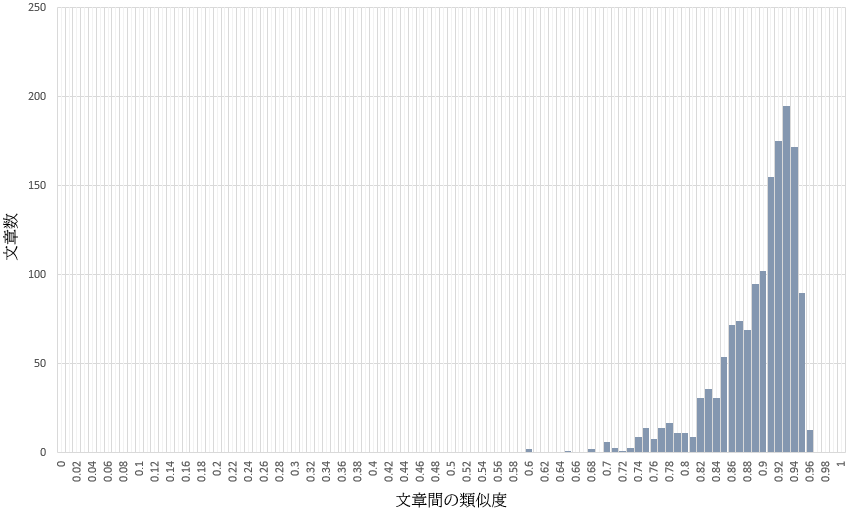
\includegraphics[width = 13.8cm]{images/みそきん類似度BERT.png}
    \caption{BERTによる類似度計算結果}
    \label{fig:みそきん類似度BERT}
\end{figure}
\vspace{10truept}

\begin{table}[ht]
    \caption{BERTによる類似度計算結果の一例}
    \vspace{5truept}

    \centering
    \begin{tabular}{|r|l|}
        \hline
        類似度結果 & 前処理済みの元コメント\\
        \hline\hline
        0.95739305 & 
        \begin{tabular}{l}
            アレルギーの関係で小麦がたくさん食べれないのでメシ版が凄く嬉しい味噌\\大好きです絶対食べます\\
        \end{tabular}\\
        \hline
        0.943691134 & 
        \begin{tabular}{l}
            味噌ラーメンからもやしメンマネギ赤い調味油って感じがくるり意識してそ\\うで好き\\
        \end{tabular}\\
        \hline
        0.939244092 & 
        \begin{tabular}{l}
            味噌ってのがいいですね食べてみます次あれば豚骨も期待してます\\
        \end{tabular}\\
        \hline
        0.936367273 & 
        \begin{tabular}{l}
            白味噌を入れることによってガツンとくる旨味が鈍くなる気がするけどどう\\なんだろうか早く買って食べたい\\
        \end{tabular}\\
        \hline
        0.914627552 & 
        \begin{tabular}{l}
            食べてみたいです楽しみ\\
        \end{tabular}\\
        \hline
        0.905122876 & 
        \begin{tabular}{l}
            今後色んな味出して欲しい\\
        \end{tabular}\\
        \hline
        0.903024077 & 
        \begin{tabular}{l}
            ファミマローソンでも販売して欲しい\\
        \end{tabular}\\
        \hline
        0.901709378 & 
        \begin{tabular}{l}
            それでも人工甘味料入ってる\\
        \end{tabular}\\
        \hline
        0.890335798 & 
        \begin{tabular}{l}
            味噌味以外も出してほしい\\
        \end{tabular}\\
        \hline
    \end{tabular}
    \label{table:みそきん類似度結果BERT}
\end{table}

\newpage
\begin{figure}[ht]
    \centering
    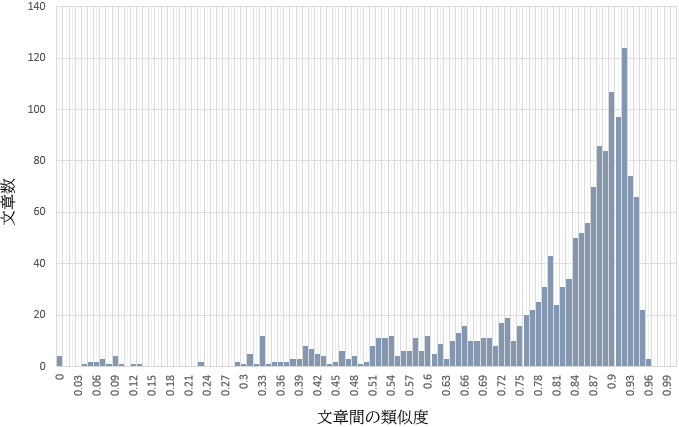
\includegraphics[width = 13.2cm]{images/みそきん類似度tf-idf.png}
    \caption{TF-IDFによる類似度計算結果}
    \label{fig:みそきん類似度tf-idf}
\end{figure}
\vspace{10truept}

\begin{table}[ht]
    \caption{TF-IDFによる類似度計算結果の一例}
    \vspace{5truept}

    \centering
    \begin{tabular}{|r|l|}
        \hline
        類似度結果 & 前処理済みの元コメント\\
        \hline\hline
        0.933934656 & 
        \begin{tabular}{l}
            味噌ってのがいいですね食べてみます次あれば豚骨も期待してます\\
        \end{tabular}\\
        \hline
        0.927453136 & 
        \begin{tabular}{l}
            アレルギーの関係で小麦がたくさん食べれないのでメシ版が凄く嬉しい味噌\\大好きです絶対食べます\\
        \end{tabular}\\
        \hline
        0.914770669 & 
        \begin{tabular}{l}
            白味噌を入れることによってガツンとくる旨味が鈍くなる気がするけどどう\\なんだろうか早く買って食べたい\\
        \end{tabular}\\
        \hline
        0.912356335 & 
        \begin{tabular}{l}
            味噌ラーメンからもやしメンマネギ赤い調味油って感じがくるり意識してそ\\うで好き\\
        \end{tabular}\\
        \hline
        0.883447275 & 
        \begin{tabular}{l}
            ファミマローソンでも販売して欲しい\\
        \end{tabular}\\
        \hline
        0.831779144 & 
        \begin{tabular}{l}
            今後色んな味出して欲しい\\
        \end{tabular}\\
        \hline
        0.800387187 & 
        \begin{tabular}{l}
            味噌味以外も出してほしい\\
        \end{tabular}\\
        \hline
        0.710342807 & 
        \begin{tabular}{l}
            食べてみたいです楽しみ\\
        \end{tabular}\\
        \hline
        0.648517863 & 
        \begin{tabular}{l}
            それでも人工甘味料入ってる\\
        \end{tabular}\\
        \hline
    \end{tabular}
    \label{table:みそきん類似度結果TF-IDF}
\end{table}

\newpage
\subsubsection{提案手法の精度検証結果}
文章間の類似度を計算し, 値が高いコメントを「商品との関連性がある」と判断するという仮説を検証するため, 
人手でアノテーションして正解ラベルを付与したデータと比較して分析を行う. 
「みそきん」のコメントに対するアノテーションは以下の基準で行った. 
アノテーションを行った結果, 「関連性-高」のラベルが付与されたコメントが934件, 「関連性-低」のラベルが付与された
コメントが541件であった. 
\vspace{10truept}

\begin{description}
    \item[関連性-高]\mbox{}
    \begin{itemize}
        \item 商品である「みそきん」に直接関係するコメント(例:味, 値段, 具など)
        \item 商品の発売日, 販売場所についてのコメント
        \item 開発過程のエピソードに関するコメント\\(例:カップラーメンを開発するために全国のラーメンを食べていたことへの興味・関心など)
        \item 「みそきん」に対する視聴者の感想・感情・意見(例:美味しそう, 絶対買う, 味噌以外も作ってほしいなど)
        \item ヒカキンのラーメン作りへのこだわり, 努力に関するコメント\\(他の視聴者の購買意欲に繋がる可能性があるため) 
    \end{itemize}
    \item[関連性-低] \mbox{}
    \begin{itemize}
        \item ラーメン作りに関係ない, ただヒカキンを褒めているコメント\\(他の視聴者が読んでラーメン作り以外の情報しか得られないもの)
        \item 視聴者自身のことを述べているコメント\\(例:所謂自分語りや〇〇店のラーメンが好きです等のコメント)
        \item その他全く関係ないコメント
    \end{itemize}
\end{description}
\vspace{10truept}

人手でアノテーションし正解ラベルを付与したデータと, 提案手法によって類似度を計算したコメントを比較し, 
提案手法の精度, 及び仮説の検証を行う. 
提案手法では類似度を計算しただけであり, 商品との関連性が高いと言える閾値は設定されていない. 
そのため, 類似度上位のコメントに対して, 人手で「関連性-高」のラベルを付与した数と同じ数のコメントだけ
「関連性-高」のラベルを付与する. 
それ以下の類似度のコメントには「関連性-低」のラベルを付与する. 
「みそきん」の場合, 正解ラベルは「関連性-高」が934件, 「関連性-低」が541件であり, 同じ数だけラベル付けした
データを用いて, 二値分類のConfusion Matrixを計算する. 
しかしこの手法ではConfusion MatrixのFP, FNの値が同じになり, Precision, Recall, 及びF1-measure
が同じ値を示してしまう(式(\ref{equation:Recall}), (\ref{equation:Precision}), (\ref{equation:F1})). 
そのため, 類似度上位25\%, 50\%, 75\%を閾値として「関連性-高」のラベルを付与したデータを作成し, 同様にConfusion Matrix
を計算することで提案手法の精度をより深く考察する. 

まず初めに, 人手の正解ラベルと同数のラベルを付与した結果について述べる. 
BERTを用いて類似度計算したデータから求めたConfusion Matrixを表\ref{table:みそきん(BERT)のconfusion}に, TF-IDFを用いて類似度計算したデータから
求めたConfusion Matrixを表\ref{table:みそきん(TF-IDF)のconfusion}に示す. 

\newpage
\begin{table}[ht]
    \centering
    \caption{みそきん(BERT)のConfusion Matrix (正解ラベルと同数のラベル付与)}
    \vspace{5truept}

    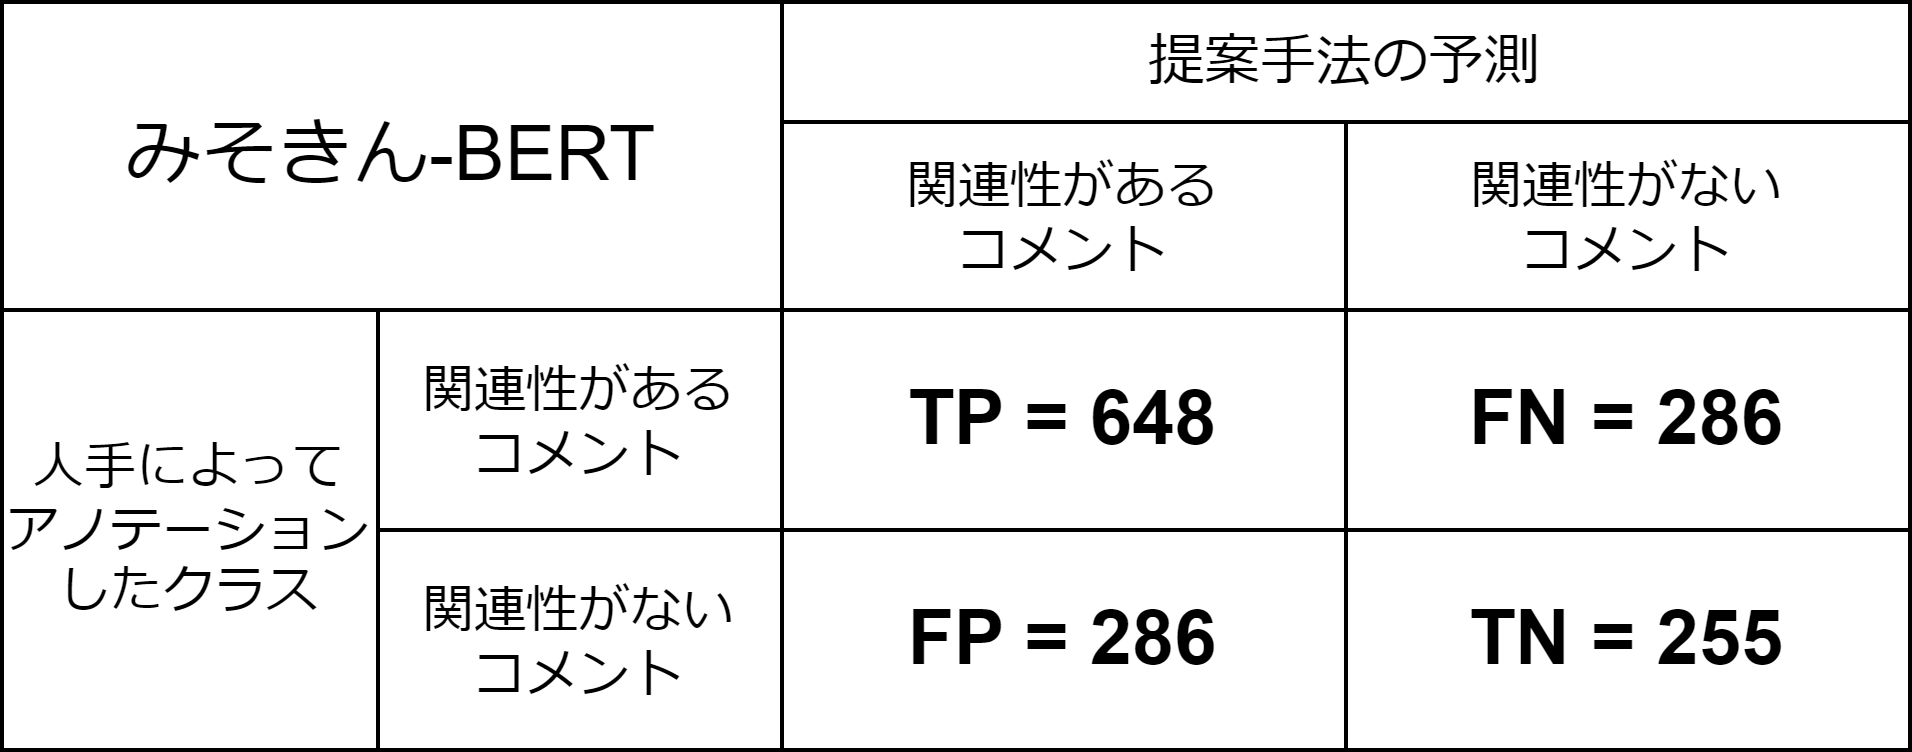
\includegraphics[width = 11cm]{images/みそきん行列.drawio.png}
    \label{table:みそきん(BERT)のconfusion}
\end{table}
\vspace{10truept}

表\ref{table:みそきん(BERT)のconfusion}のConfusion Matrixから各指標を計算すると以下のような結果が得られる. 
この結果より,  「みそきん」に対する提案手法の全体的な正解率はAccuracy = 0.6122であることが分かった. 
Recall, Precision, F1-measure = 0.6938であり, 提案手法で予測した関連性があるコメントが約7割正解していること, 
また人手で関連性があると判断したコメントのうち約7割が提案手法でも関連性ありと予測されていることが分かる. 
\vspace{10truept}

\begin{equation}
    \textrm{Accuracy} = \dfrac{TP+TN}{TP+FP+FN+TN} = 0.612203...
\end{equation}
\vspace{5truept}

\begin{equation}
    \textrm{Sensitivity・Recall} = \dfrac{TP}{TP+FN} = 0.693790...
\end{equation}
\vspace{5truept}

\begin{equation}
    \textrm{Precision} = \dfrac{TP}{TP+FP} = 0.693790...
\end{equation}
\vspace{5truept}

\begin{equation}
    \textrm{F1-measure} = \dfrac{2\times \textrm{Precision}\times \textrm{Recall}}{\textrm{Precision}+\textrm{Recall}} = \dfrac{2\times TP}{2\times TP+FP+FN} = 0.693790...
\end{equation}
\vspace{10truept}

\begin{table}[ht]
    \centering
    \caption{みそきん(TF-IDF)のConfusion Matrix (正解ラベルと同数のラベル付与)}
    \vspace{5truept}

    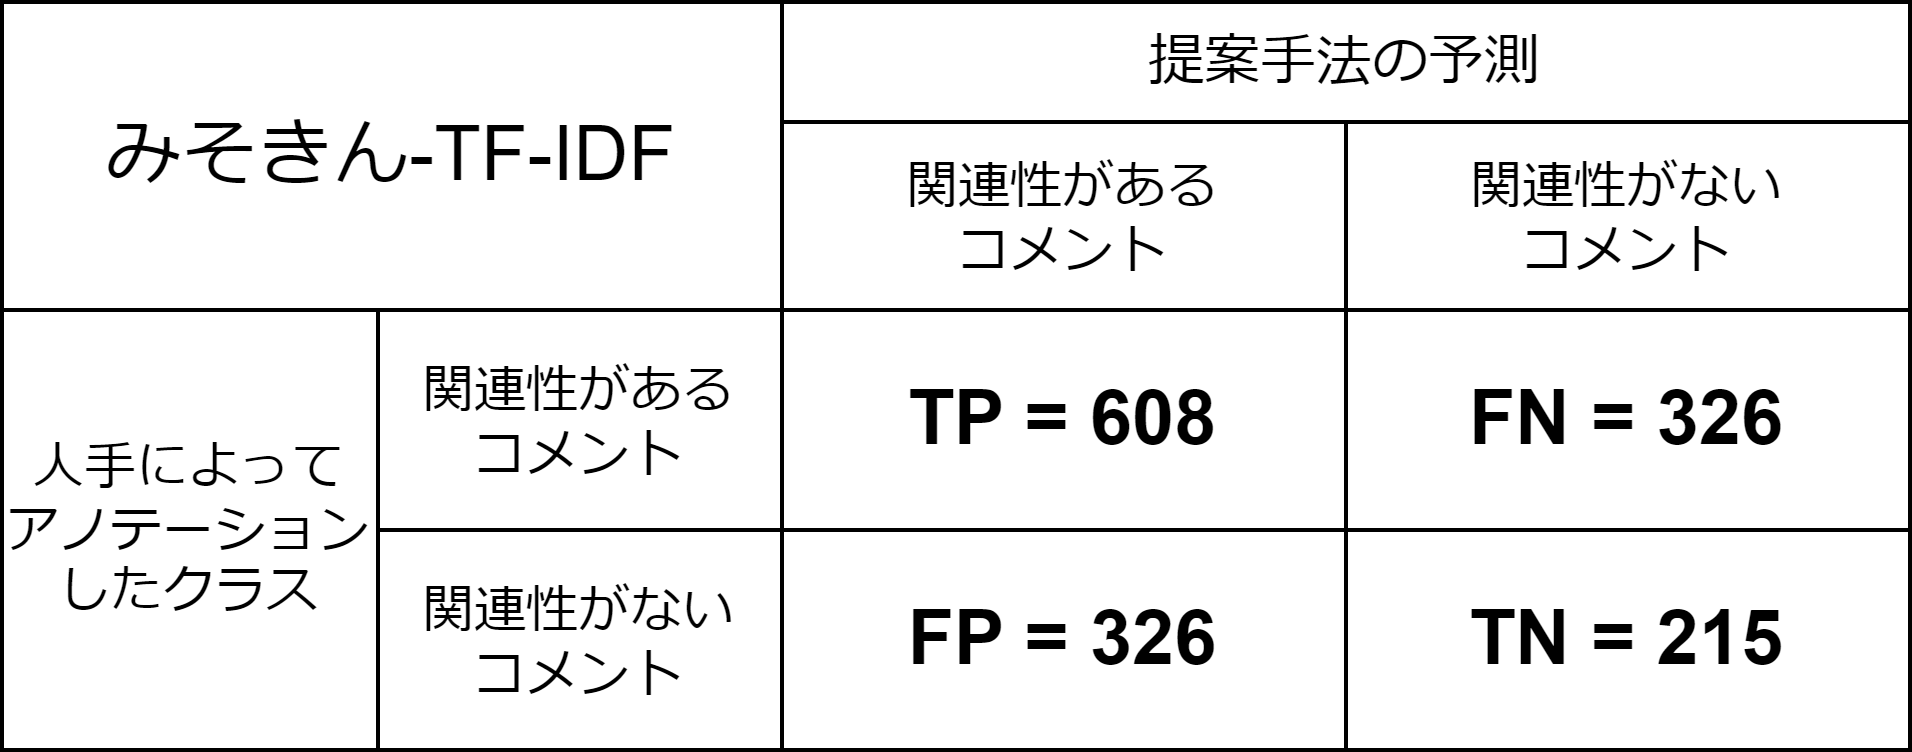
\includegraphics[width = 11cm]{images/みそきん行列tf-idf.drawio.png}
    \label{table:みそきん(TF-IDF)のconfusion}
\end{table}

\newpage
表\ref{table:みそきん(TF-IDF)のconfusion}のConfusion Matrixから各指標を計算すると以下のような結果が得られる. 
TF-IDFを用いて類似度計算したデータを用いた場合全体の正解率は0.5580となり, BERTを用いて類似度計算したデータよりも低い値を示した. 
また, Recall, Precision, F1-measureも同様にBERTに比べて低く, 提案手法で予測したコメントのうち約6.5割が実際に
関連性があるコメントであること, また人手で関連性ありと判断したコメントのうち約6.5割が提案手法でも関連性ありと予測された結果となった. 
\vspace{10truept}

\begin{equation}
    \textrm{Accuracy} = \dfrac{TP+TN}{TP+FP+FN+TN} = 0.557966...
\end{equation}
\vspace{5truept}

\begin{equation}
    \textrm{Sensitivity・Recall} = \dfrac{TP}{TP+FN} = 0.650963...
\end{equation}
\vspace{5truept}

\begin{equation}
    \textrm{Precision} = \dfrac{TP}{TP+FP} = 0.650963...
\end{equation}
\vspace{5truept}

\begin{equation}
    \textrm{F1-measure} = \dfrac{2\times \textrm{Precision}\times \textrm{Recall}}{\textrm{Precision}+\textrm{Recall}} = \dfrac{2\times TP}{2\times TP+FP+FN} = 0.650963...
\end{equation}
\vspace{10truept}

次に, 各類似度計算法によって計算した文章間の類似度の上位25\%, 50\%, 75\%に対して「関連性-高」のラベルを付与して
同様の実験を行った結果を表\ref{table:みそBERT閾値}に示す. 
Accuracyを見ると, 閾値をどの値に設定しても全体的な正解率は50\%を超えていることが分かる. 
Precisionは閾値を低く設定するにつれて値が低くなるが, 一番低い75\%の場合でも0.66あり, どの閾値に設定した場合でも
提案手法で予測したコメントのうち約6.6割以上が正解していることが分かる. 
閾値を低く設定するにつれてPrecisionが低くなるのは, 誤って「関連性-高」と判断するコメントが増えるからであると考えられる. 
Precisonとは逆にRecallは閾値を低く設定するにつれて値が高くなった. 
これは「関連性-高」と判断するコメントが多くなると, その取りこぼし(「関連性-高」を「関連性-低」と判断する事象)
が少なくなるからであると考えられる. 
Recallの値は閾値25\%のときに約3割であり, 提案手法の性能としては満足できない結果であるが, 
閾値75\%のときは約8割で取りこぼしなく関連性があるコメントを抽出できていることが分かる. 
\vspace{5truept}

\begin{table}[ht]
    \centering
    \caption{「関連性-高」の閾値を上位25\%, 50\%, 75\%に設定した結果 (BERT)}
    \vspace{5truept}

    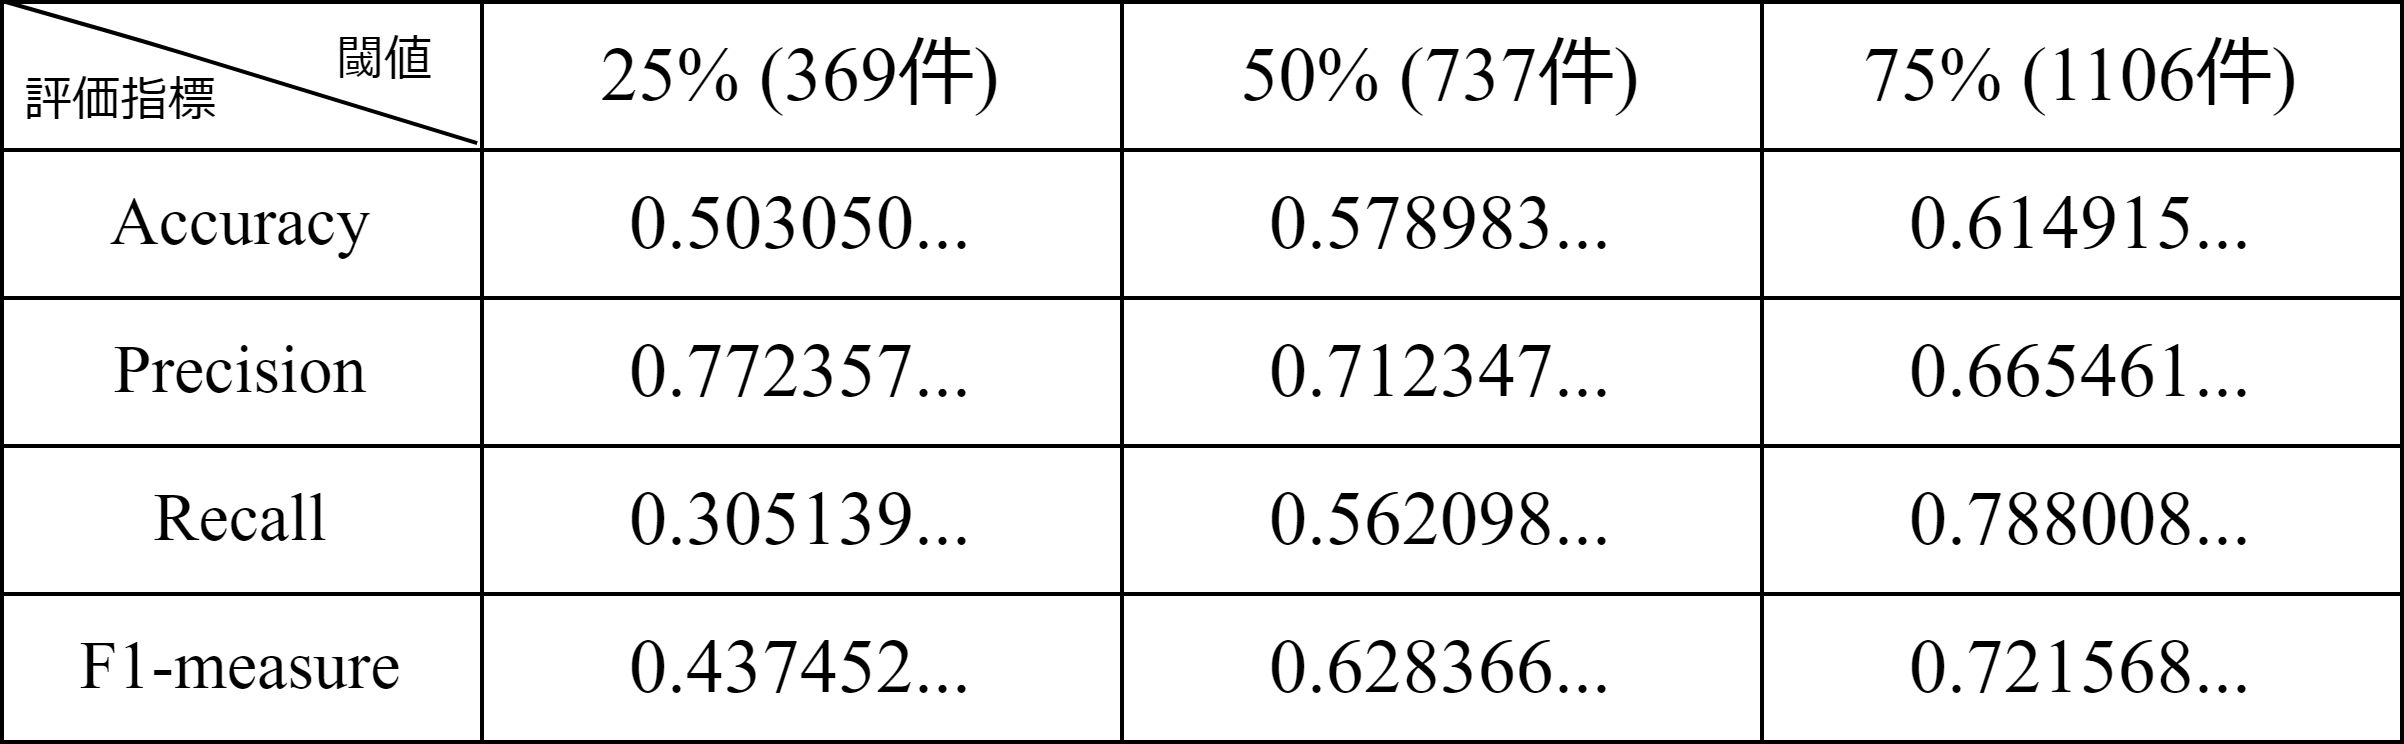
\includegraphics[width = 14cm]{images/BERT25.drawio.png}
    \label{table:みそBERT閾値}
\end{table}
\noindent
F1-measureはPrecisionとRecallの調和平均であり, Accuracyと同様に全体的な提案手法の性能を測ることができる. 
閾値25\%では5割を切っているため閾値として適切ではないことが分かる. 
閾値75\%のときにF1-measureは最大となるが, Precisionは閾値設定を行わずに正解ラベルと同数のラベルを付与したときの方が
値が高いため, PrecisionとF1-measure(Recall)のどちらを優先するかは考察の余地がある. 

次に, TF-IDFを用いて類似度計算したデータに閾値を設定してラベルを付与した結果から計算した各指標を表\ref{table:みそTF-IDF閾値}に示す. 
BERTでの結果(表\ref{table:みそBERT閾値})と比較すると, 対応する全ての値が低いことが分かる. 
また, 閾値を低くするにつれてPrecisionが低くなることや, Recall・F1-measureが高くなることなどは一致しており, 
類似度計算法による差異は値のみであることが分かった. そのため, 本研究に対してより有効な類似度計算法はBERTで文章をベクトル化
し, Cos類似度を計算する方法であると考えられる. 

\vspace{10truept}

\begin{table}[h]
    \centering
    \caption{「関連性-高」の閾値を上位25\%, 50\%, 75\%に設定した結果 (TF-IDF)}
    \vspace{5truept}

    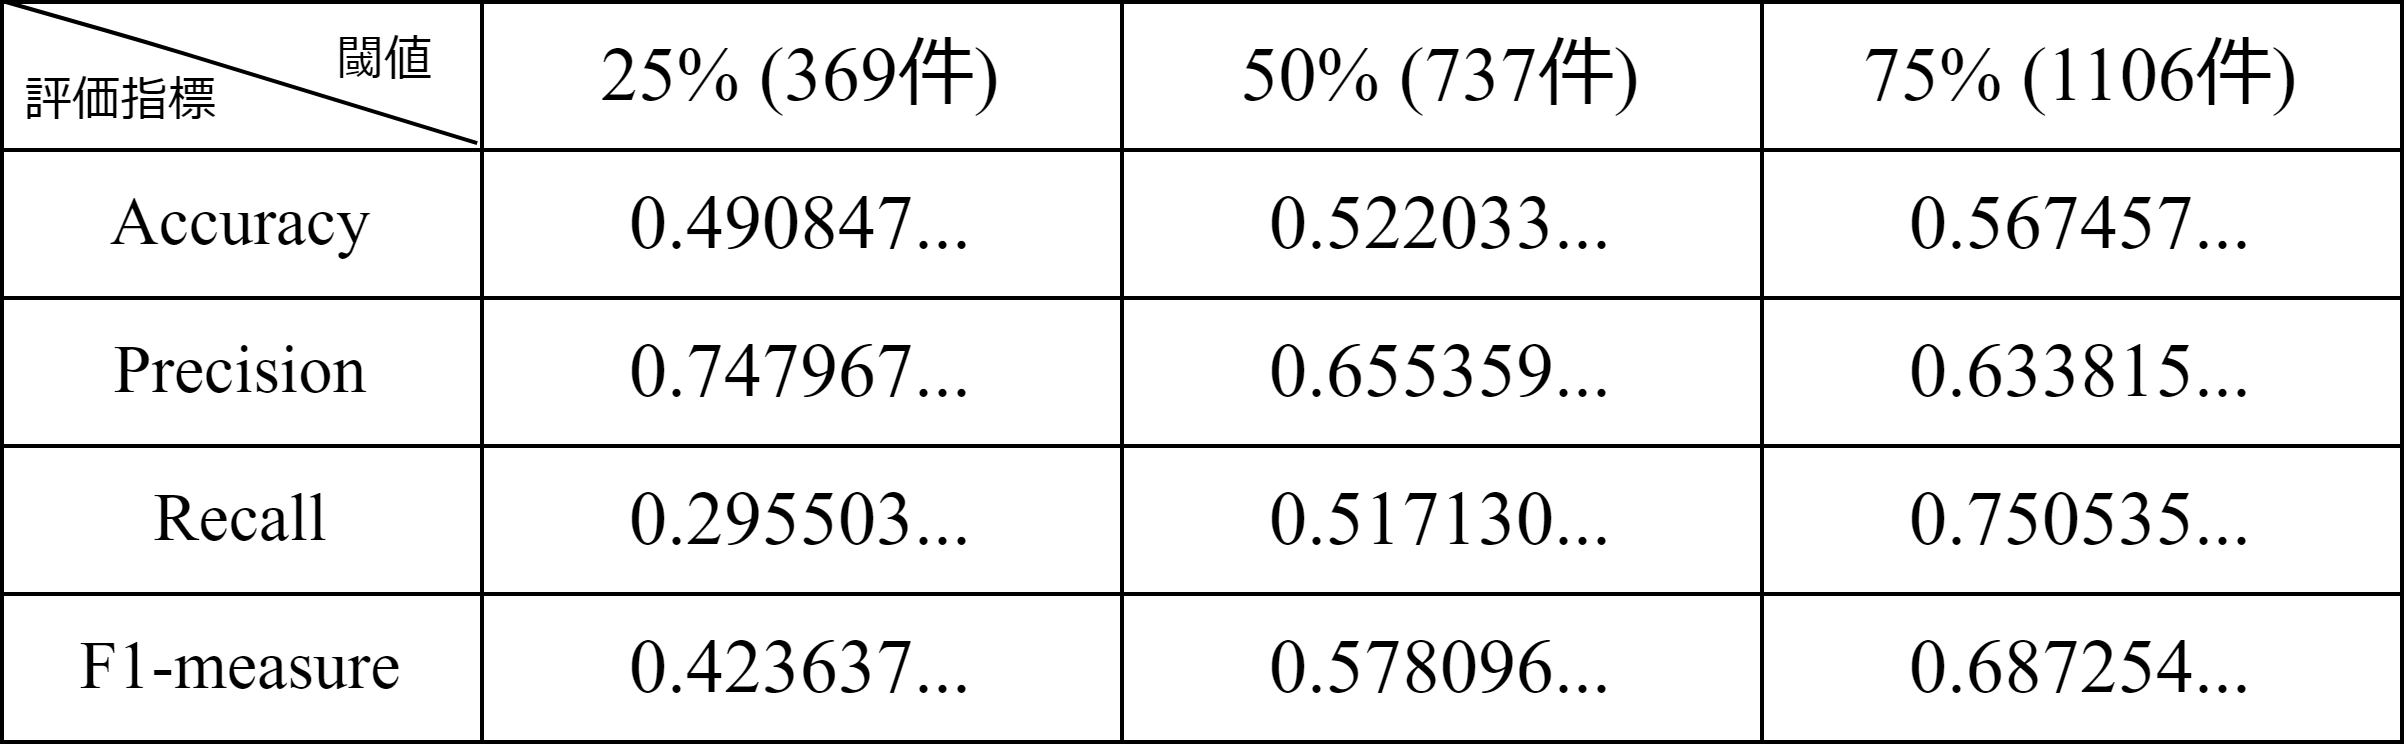
\includegraphics[width = 14cm]{images/TF-IDF閾値.drawio.png}
    \label{table:みそTF-IDF閾値}
\end{table}
\subsubsection{LDAとの比較}
提案手法で用いているBTMが代表的なトピックモデルであるLDAと比べて優れているかどうかを検証する. 
BTMを用いてトピック推定, 及び単語抽出を行った過程(6.1.1節)をLDAで行い, その後は同様の手法で実験を行った. 
表\ref{table:みそきん単語結果LDA}にLDAを用いてトピック推定を行い, トピックごとの出現確率上位10単語を抽出した結果を示す. 
BTMと同様に商品に関連している単語を多く抽出
\begin{table}[h]
    \caption{LDAで抽出した単語リスト(みそきん)}
    \vspace{5truept}

    \centering
    \begin{tabular}{|c|>{\centering}p{6em}|>{\centering}p{6em}|>{\centering}p{6em}|>{\centering}p{6em}|>{\centering\arraybackslash}p{6em}|}
        \hline
        & Topic 0 & Topic 1 & Topic 2 & Topic 3 & Topic 4\\
        \hline\hline
        1 & ラーメン & 0 & 0 & まずい & 絶対\\
        \hline
        2 & ヒカキン & ラーメン & ヒカキン & ヒカキン & hikakin\\
        \hline
        3 & 好き & ー & ヒカキン & 夢 & ラーメン\\
        \hline
        4 & 夢 & 嬉しい & 夢 & 美味しかっ & 美味し\\
        \hline
        5 & hikakin & 味 & 姿 & すごい & 夢\\
        \hline
        6 & 凄い & ラーメン & キン & ラーメン & 楽しみ\\
        \hline
        7 & 努力 & みそ & 売り切れ & youtube & 0\\
        \hline
        8 & 商品 & 報告 & 尊敬 & 努力 & セブン\\
        \hline
        9 & 尊敬 & 美味しかっ & hikakin & 尊敬 & 大好き\\
        \hline
        10 & 凄 & コンビニ & 嬉しい & hikakin & 発売\\
        \hline
    \end{tabular}
    \label{table:みそきん単語結果LDA}
\end{table}
できているが, BTMとは異なり「0」や「ー」など, 数字や記号がいくつか抽出されている結果となった. 
その後, 表\ref{table:みそきん類似度結果BERT}の単語を用いて文章を生成し, BERTによる文章のベクトル化を用いた類似度計算を行った. 
6.1.4節で元のコメントに正解ラベルを付与したデータと, 同じ件数のラベルを付与した予測データからConfusion Matrixと各指標を
計算した結果を表\ref{table:みそきんLDA_Confusion}に示す. 
BTMを用いた手法の結果(表\ref{table:みそきん(BERT)のconfusion})と比較すると, LDAを用いた手法では正しく予測している
TPとTNが減り, 誤った予測をしているFPとFNが増加している. 
それに伴い, 計算した各指標もBTMの結果に比べて少し低くなっている. 
このことから, 短いテキストに対するトピック推定及び単語抽出はLDAよりもBTMの方が優れていること, また
提案手法で用いるトピックモデルとしてもBTMの方が優れていると考えられる. 

\vspace{10truept}

\begin{table}[h]
    \centering
    \caption{LDAを用いた手法のConfusion Matrix}
    \vspace{5truept}

    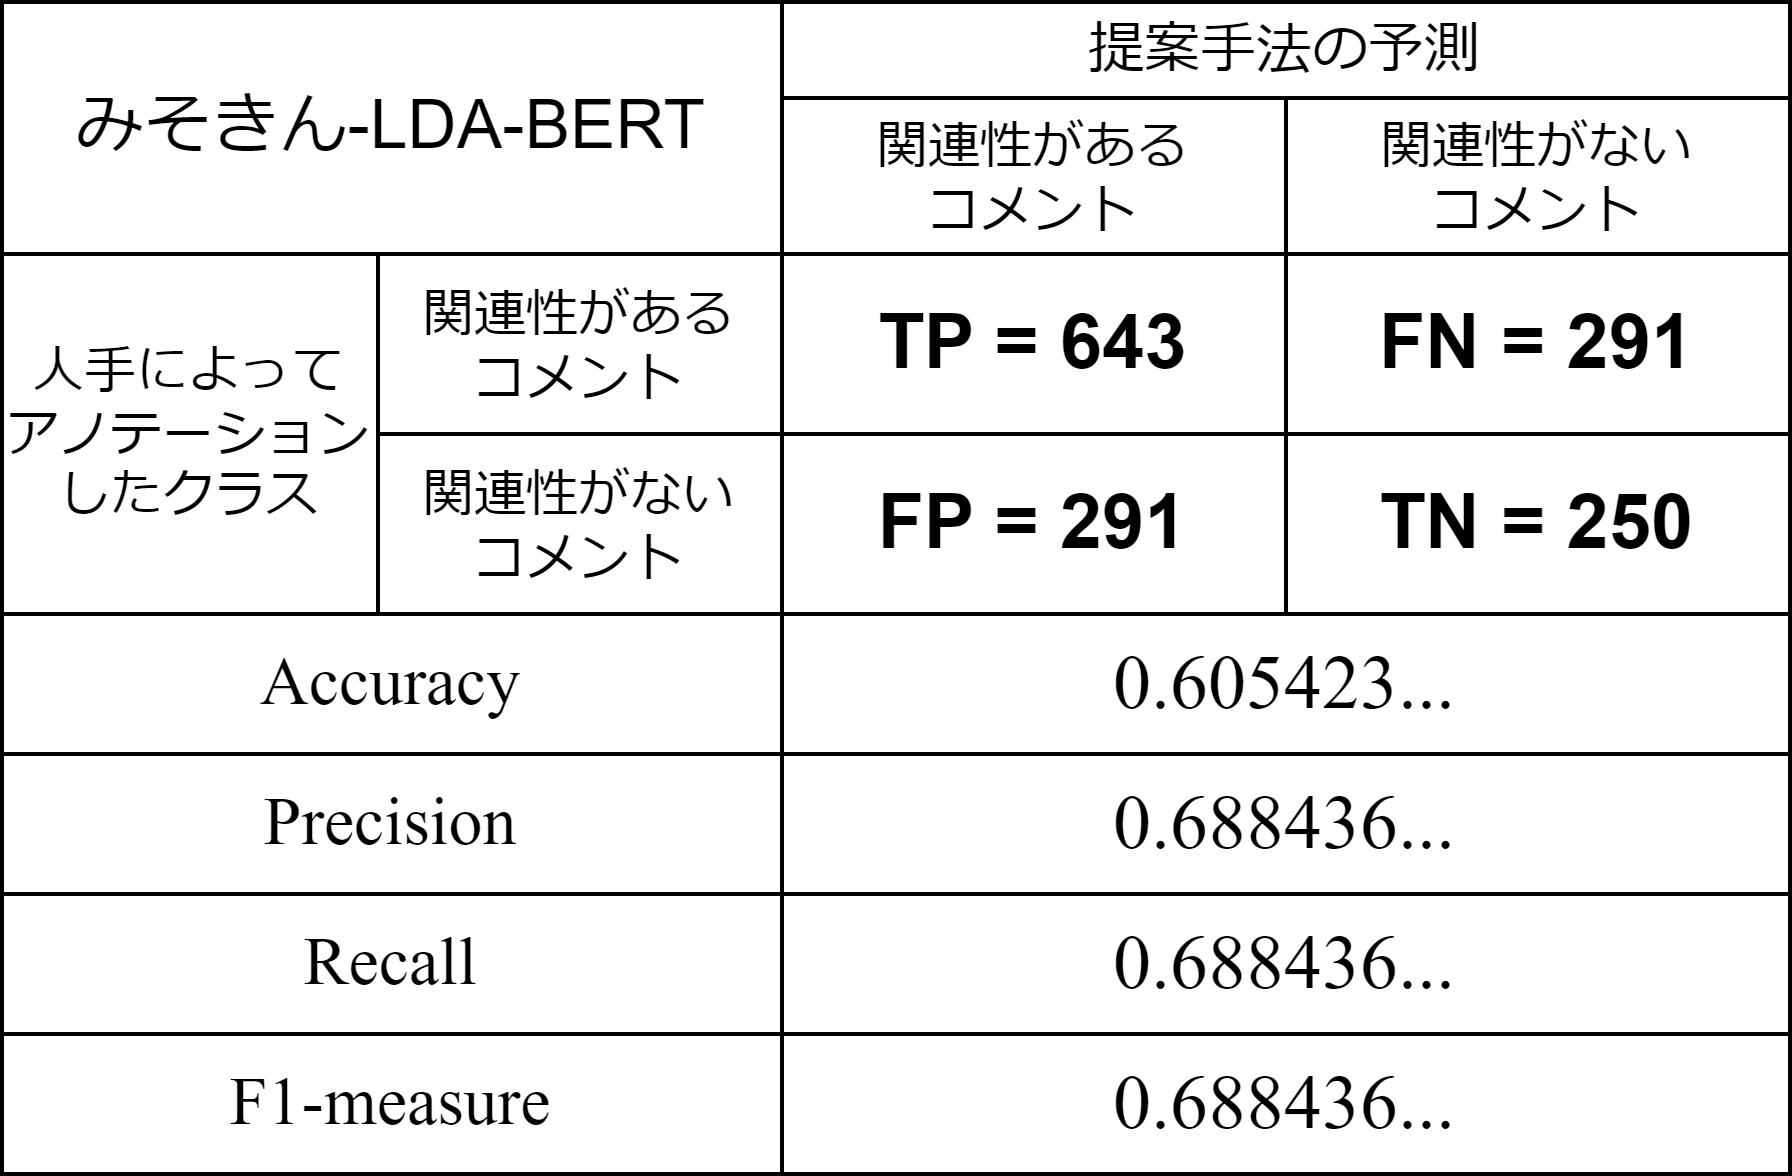
\includegraphics[width = 12cm]{images/みそきんLDA.drawio.png}
    \label{table:みそきんLDA_Confusion}
\end{table}

\subsection{豚汁のレシピ紹介動画}
料理研究家のリュウジが自身のYouTubeチャンネルで投稿した豚汁のレシピ, 及び調理過程の動画[8](以下「豚汁」)からコメントを抽出した. 
以下に詳細な実験条件を示す. 
\begin{description}
    \item[コメント件数]\mbox{}\\
    抽出したコメントは1337件であり, そこから前処理・分かち書きの過程で削除された文章(絵文字のみの文章や一文字のみの文章)
    を除いた1306件を用いてBTMで分析した. 人手によるアノテーション, 及び類似度計算に用いるコメントは前処理のみを施した
    コメント1329件を用いた. 

    \item[前処理] \mbox{}\\
    前処理の形態素解析の段階では「名詞」と「形容詞」のみを抽出し分かち書きを行った. 
    \item[BTMの各パラメータ]\mbox{}
    \begin{itemize}
        \item トピック数 $T=5$
        \item 単語分布から抽出する出現確率上位の単語数 $n = 10$
        \item 各文章ごとに考慮する単語数 $M=10$
        \item 反復回数 $\textrm{iterations} = 20$
        \item ディリクレ分布のハイパーパラメータ $\alpha, \beta$\\
        他の実験と同じ手法でハイパーパラメータを調整した. 
        「豚汁」では$\alpha = 0.93, \beta = 0.1$で実験を行った. 
    \end{itemize}
\end{description}
\subsubsection{BTMによって抽出した単語リスト}
上位の条件に従って実験を行い, BTMによって抽出した出力確率上位10単語を表\ref{table:豚汁単語結果}に示す. 
表\ref{table:豚汁単語結果}から読み取れる通り, 動画投稿者の料理研究家である「リュウジ」や調理している「豚汁」, 
豚汁の具材である「ゴボウ」, 「大根」, 豚汁の味にかかわる「味噌」, 「ニンニク」などの単語がBTMによって推定したトピックに出現しやすい
単語であることが分かる. コメント集合を把握した上で他の出力されている単語を見ると, このレシピが「美味しい」や「最高」などの視聴者の感情
を表している単語や, この動画を見て「家族」に「今日」「作りました」などの単語が多く出力されているため, 適切に単語を抽出できていることが分かった. 
トピック間で単語を見ていくと, Topic 0\sim3では「豚汁」, 「リュウジ」, 「美味しい」, 「レシピ」が共通して出現していて, 
リュウジが紹介しているレシピで豚汁を作った感想に関するトピックが推定されていると考えられる. 
Topic 4ではほぼすべての単語が豚汁の具や味など, レシピの内容に関わる単語を抽出しているため, 豚汁のレシピに関するトピックであると判断することができる. 


\vspace{10truept}

\begin{table}[h]
    \caption{BTMで抽出した単語リスト(豚汁)}
    \vspace{5truept}

    \centering
    \begin{tabular}{|c|>{\centering}p{6em}|>{\centering}p{6em}|>{\centering}p{6em}|>{\centering}p{6em}|>{\centering\arraybackslash}p{6em}|}
        \hline
        & Topic 0 & Topic 1 & Topic 2 & Topic 3 & Topic 4\\
        \hline\hline
        1 & 豚汁 & 豚汁 & 豚汁 & 料理 & 豚汁\\
        \hline
        2 & レシピ & 美味しい & 至高 & リュウジ & 野菜\\
        \hline
        3 & リュウジ & 美味しく & レシピ & 動画 & ゴボウ\\
        \hline
        4 & 美味しい & リュウジ & リュウジ & 最高 & 味噌\\
        \hline
        5 & 料理 & 味噌 & 大好き & 豚汁 & 白だし\\
        \hline
        6 & 動画 & 生姜 & 今日 & 美味しい & 生姜\\
        \hline
        7 & 作りました & 味噌汁 & 美味しかっ & 好き & ニンニク\\
        \hline
        8 & 最高 & 作りました & 美味しい & 兄さん & 料理\\
        \hline
        9 & 美味しく & レシピ & 料理 & レシピ & 大根\\
        \hline
        10 & 今日 & ニンニク & シリーズ & 家族 & ネギ\\
        \hline
    \end{tabular}
    \label{table:豚汁単語結果}
\end{table}

\subsubsection{文章生成}
表\ref{table:豚汁単語結果}に示している単語を使って, ChatGPT(GPT-4)を用いて文章を生成した結果を示す. 
ChatGPTに入力したプロンプトは以下の通りである.  「豚汁」では料理研究家の「リュウジ」を人名とする以外は5.4節で述べた通りのプロンプトを入力した. 
\begin{itemize}
    \item 空白区切りで入力する単語を使って文章を生成してください.
    \item 全ての単語を使用してください.
    \item YouTubeのコメントにあるような文章を生成してください.
    \item 可能な限り短い文章を生成してください.
    \item ``リュウジ''は人名として扱ってください.
\end{itemize}
\vspace{10truept}

上記のプロンプトとBTMで得られた各トピックの出現確率上位の単語をChatGPTに入力して文章を生成した結果を表\ref{table:豚汁生成結果}に示す. 
「みそきん」の文章生成の結果(表\ref{table:みそきん生成結果})と比較すると, 文章がより自然で伝わりやすく, さらに短い文章が
生成されていると思われる. これは単語抽出結果(表\ref{table:豚汁単語結果})も「みそきん」より対象の動画と関連している単語
を抽出できていることに起因していると考えられる. 
\vspace{5truept}

\begin{table}[h]
    \caption{ChatGPTによる文章生成結果 (豚汁)}
    \vspace{5truept}

    \centering
    \begin{tabular}{|c|l|}
        \hline
        & 生成結果\\
        \hline\hline
        Topic 0 & 
        \begin{tabular}{l}
            今日、リュウジの料理動画を見て豚汁のレシピを作りました!\\最高に美味しくて、美味しいです!
        \end{tabular}\\
        \hline
        Topic 1 & 
        \begin{tabular}{l}
            リュウジのレシピで作った豚汁、美味しい!\\生姜とニンニクが効いた味噌汁、本当に美味しくて最高!
        \end{tabular}\\
        \hline
        Topic 2 &
        \begin{tabular}{l}
            今日、リュウジのレシピで豚汁を作りました。\\至高の味で、大好きな料理シリーズがまた一つ増えました!美味しかった!
        \end{tabular}\\
        \hline
        Topic 3 &
        \begin{tabular}{l}
            リュウジ兄さんの動画を見て料理した豚汁、家族にも大好評!\\本当に美味しいレシピでした。最高です!
        \end{tabular}\\
        \hline
        Topic 4 &
        \begin{tabular}{l}
            豚汁にゴボウ、大根、ネギをたっぷり使い、味噌と白だしで味付け。\\生姜とニンニクで風味豊かな料理になりました!
        \end{tabular}\\
        \hline
    \end{tabular}
    \label{table:豚汁生成結果}
\end{table}

\subsubsection{二種の類似度計算法による結果}
ChatGPT(GPT-4)で生成した文章と, 前処理を施した元のYouTubeのコメントとの文章間の類似度を計算した結果を述べる. 
「みそきん」と同様にBERTとTF-IDFによる文章のベクトル化を用いてCos類似度を計算し, 二つの手法がどのような特徴を
持っているかを考察する. 
図\ref{fig:豚汁類似度BERT}, \ref{fig:豚汁類似度TF-IDF}は各類似度計算法によって算出した文章間の類似度をグラフ化したものである. 
「みそきん」の結果と同様に, BERTを用いた手法ではほとんどのコメントが0.7\sim0.96の値を取っている. 
しかし, TF-IDFを用いた手法では「みそきん」と比べて0\sim0.7の値を持つコメントの数が少ないことが図\ref{fig:豚汁類似度TF-IDF}
から分かった. これは「豚汁」の文章生成の精度が「みそきん」に比べて高いことと, 「豚汁」の動画に対する元のコメント
が「みそきん」に比べて商品(レシピ)に関連するものが多いことが起因していると考えられる. 表\ref{table:豚汁類似度結果BERT}, 
\ref{table:豚汁類似度結果TF-IDF}はそれぞれの類似度計算法の結果の一例であり, 後に人手でアノテーションする際には
「関連性-高」と判断されるコメントである. 
表\ref{table:豚汁類似度結果TF-IDF}では長さが短い文章のときに類似度が低くなってしまっているが, 
同じコメントに対して表\ref{table:豚汁類似度結果BERT}では類似度が高く算出されている. 
この結果より, BERTを用いた手法の方が短い文章でも適切に文章間の類似度を測れているといえる. 




\newpage
\begin{figure}[ht]
    \centering
    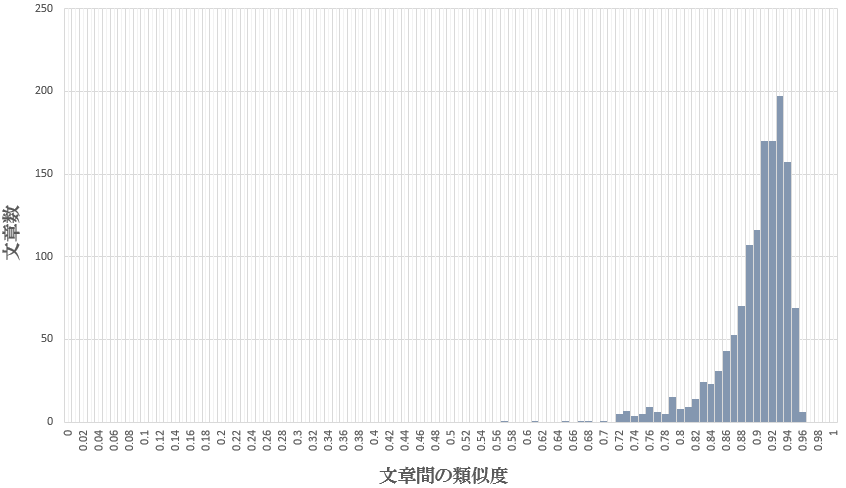
\includegraphics[width = 14.4cm]{images/豚汁images/豚汁類似度BERT.png}
    \caption{BERTによる類似度計算結果}
    \label{fig:豚汁類似度BERT}
\end{figure}
\vspace{30truept}

\begin{table}[ht]
    \caption{BERTによる類似度計算結果の一例}
    \vspace{5truept}

    \centering
    \begin{tabular}{|r|l|}
        \hline
        類似度結果 & 前処理済みの元コメント\\
        \hline\hline
        0.955579638 & 
        \begin{tabular}{l}
            このレシピのお陰で豚肉入り味噌汁から卒業出来ました流石至高ですね\\美味しいし娘に伝授します\\
        \end{tabular}\\
        \hline
        0.945638359 & 
        \begin{tabular}{l}
            今日このレシピで豚汁作ったら家族に大好評でしたすごく美味しかったです\\
        \end{tabular}\\
        \hline
        0.938940465 & 
        \begin{tabular}{l}
            ほんとに美味しい最後のニンニク最高今からの季節これで決まりいつも\\美味しいレシピありがとうございます\\
        \end{tabular}\\
        \hline
        0.93707478 & 
        \begin{tabular}{l}
            ゴボウがこんなに美味しいなんて豚汁のごぼうは鬼門だったのですが香り\\高くて味が染みて豚の脂も味噌も吸って美味しい目からウロコでした\\ゴボウ探して食べました至高シリーズまた待ってます\\
        \end{tabular}\\
        \hline
        0.930768073 & 
        \begin{tabular}{l}
            これは美味いニンニクと生姜が良かったです\\
        \end{tabular}\\
        \hline
        0.92407757 & 
        \begin{tabular}{l}
            これ本当に美味しくてリピートしまくってます\\
        \end{tabular}\\
        \hline
        0.886364281 & 
        \begin{tabular}{l}
            さつまいも入れても美味しかった\\
        \end{tabular}\\
        \hline
        0.842903078 & 
        \begin{tabular}{l}
            ニンニクが強いかも\\
        \end{tabular}\\
        \hline
    \end{tabular}
    \label{table:豚汁類似度結果TF-IDF}
\end{table}


\newpage
\begin{figure}[ht]
    \centering
    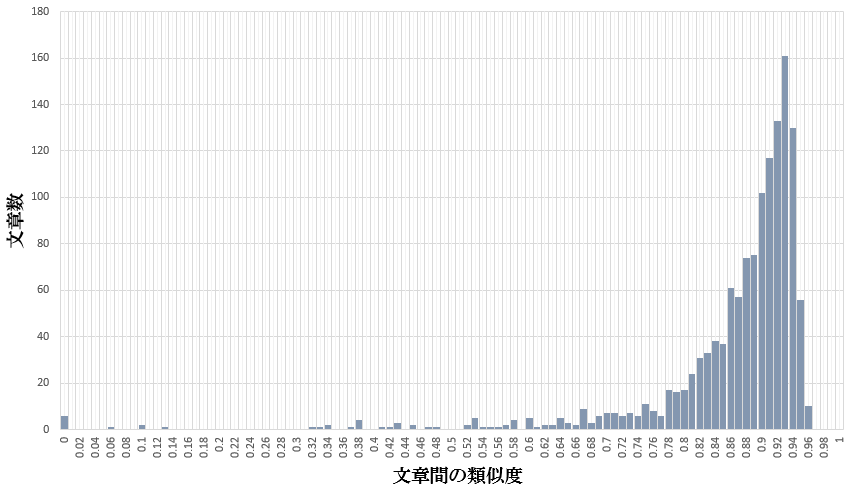
\includegraphics[width = 14.4cm]{images/豚汁images/豚汁類似度TF-IDF.png}
    \caption{TF-IDFによる類似度計算結果}
    \label{fig:豚汁類似度TF-IDF}
\end{figure}
\vspace{30truept}

\begin{table}[ht]
    \caption{TF-IDFによる類似度計算結果の一例}
    \vspace{5truept}

    \centering
    \begin{tabular}{|r|l|}
        \hline
        類似度結果 & 前処理済みの元コメント\\
        \hline\hline
        0.940920903 & 
        \begin{tabular}{l}
            このレシピのお陰で豚肉入り味噌汁から卒業出来ました流石至高ですね\\美味しいし娘に伝授します\\
        \end{tabular}\\
        \hline
        0.926962319 & 
        \begin{tabular}{l}
            ゴボウがこんなに美味しいなんて豚汁のごぼうは鬼門だったのですが香り\\高くて味が染みて豚の脂も味噌も吸って美味しい目からウロコでした\\ゴボウ探して食べました至高シリーズまた待ってます\\
        \end{tabular}\\
        \hline
        0.910778972 & 
        \begin{tabular}{l}
            今日このレシピで豚汁作ったら家族に大好評でしたすごく美味しかったです\\
        \end{tabular}\\
        \hline
        0.896905186 & 
        \begin{tabular}{l}
            ほんとに美味しい最後のニンニク最高今からの季節これで決まりいつも\\美味しいレシピありがとうございます\\
        \end{tabular}\\
        \hline
        0.889494581 & 
        \begin{tabular}{l}
            これは美味いニンニクと生姜が良かったです\\
        \end{tabular}\\
        \hline
        0.813619133 & 
        \begin{tabular}{l}
            これ本当に美味しくてリピートしまくってます\\
        \end{tabular}\\
        \hline
        0.676619315 & 
        \begin{tabular}{l}
            さつまいも入れても美味しかった\\
        \end{tabular}\\
        \hline
        0.594438816 & 
        \begin{tabular}{l}
            ニンニクが強いかも\\
        \end{tabular}\\
        \hline
    \end{tabular}
    \label{table:豚汁類似度結果BERT}
\end{table}

\newpage
\subsubsection{提案手法の精度検証結果}
文章間の類似度を計算し, その値が高いコメントを「商品(豚汁のレシピ)との関連性がある」と判断するという仮説を検証するため, 
人手でアノテーションして正解ラベルを付与したデータと比較して分析を行う. 
「豚汁」のコメントに対するアノテーションは以下の基準で行った. アノテーションを行った結果, 「関連性-高」のラベルが付与された
コメントが882件, 「関連性-低」のラベルが付与されたコメントが447件であった. 
\vspace{10truept}

\begin{description}
    \item[関連性-高]\mbox{}
    \begin{itemize}
        \item 紹介している豚汁のレシピに直接関係するコメント(例:具, 味付け, 調味料)
        \item 実際に豚汁を作った視聴者のレシピに対する感想(例:美味しかった, 家族に喜んでもらえた)
        \item アレンジをした視聴者のコメント(例:里芋を入れた方が美味しかった)
        \item 調理方法に関連するコメント(例:ねぎの切り方, 茹で時間)
    \end{itemize}
    \item[関連性-低] \mbox{}
    \begin{itemize}
        \item レシピには関係ないが動画内容に関係しているコメント(例:飲酒しながら撮影していることに対するコメント)
        \item 動画投稿者の他の料理動画に対するコメント(例:〇〇のレシピを教えてほしい)
        \item 視聴者自身のことを述べているコメント(例:ゴボウ買い忘れた, ハイボール飲みたくなる)
        \item その他全く関係ないコメント
    \end{itemize}
\end{description}
\vspace{10truept}

人手でアノテーションし正解ラベルを付与したデータと, 提案手法によって類似度を計算したコメントを比較し, 
提案手法の精度, 及び仮説の検証を行う. 
提案手法では類似度を計算しただけであり, 商品との関連性が高いと言える閾値は設定されていない. 
そのため, 類似度上位のコメントに対して, 人手で「関連性-高」のラベルを付与した数と同じ数のコメントだけ
「関連性-高」のラベルを付与する. 
それ以下の類似度のコメントには「関連性-低」のラベルを付与する. 
「豚汁」の場合, 正解ラベルは「関連性-高」が882件, 「関連性-低」が447件であり, 同じ数だけラベル付けした
データを用いて, 二値分類のConfusion Matrixを計算する. 
また, 「みそきん」と同様に類似度上位25\%, 50\%, 75\%を閾値として「関連性-高」のラベル
を付与したデータを作成し, 同様にConfusion Matrixを計算することで提案手法の精度をより深く考察する. 

まず初めに, 人手の正解ラベルと同数のラベルを付与した結果について述べる. 
BERTを用いて類似度計算したデータから求めたConfusion Matrixを表\ref{table:豚汁(BERT)のconfusion同件数}に, 
TF-IDFを用いて類似度計算したデータから求めたConfusion Matrixを表\ref{table:豚汁(TF-IDF)のconfusion同件数}に示す. 
表\ref{table:豚汁(BERT)のconfusion同件数}より, 「豚汁」に対する提案手法の全体的な正解率はAccuracy=0.703536であり, 
「みそきん」よりも正解率が高いことが分かった. また, Precision, Recall, F1-measure=0.776643であり, 同様に「みそきん」
よりも高い精度でコメントを分類できていることが分かった. Precisionが0.776643であることから, 
提案手法で予測したコメントのうち約7.7割が人手で関連性があると判断したコメントであることが分かり, 提案手法に有用性があると判断することができると思われる. 
Recallも同様に0.776643であり, 人手で関連性があると判断したコメントのうち約7.7割が提案手法で関連性があると予測されているため, 
他のユーザーにとって有益なコメントの取りこぼしが少ないといえる. 
\newpage
\begin{table}[ht]
    \centering
    \caption{豚汁(BERT)のConfusion Matrix (正解ラベルと同数のラベル付与)}
    \vspace{5truept}

    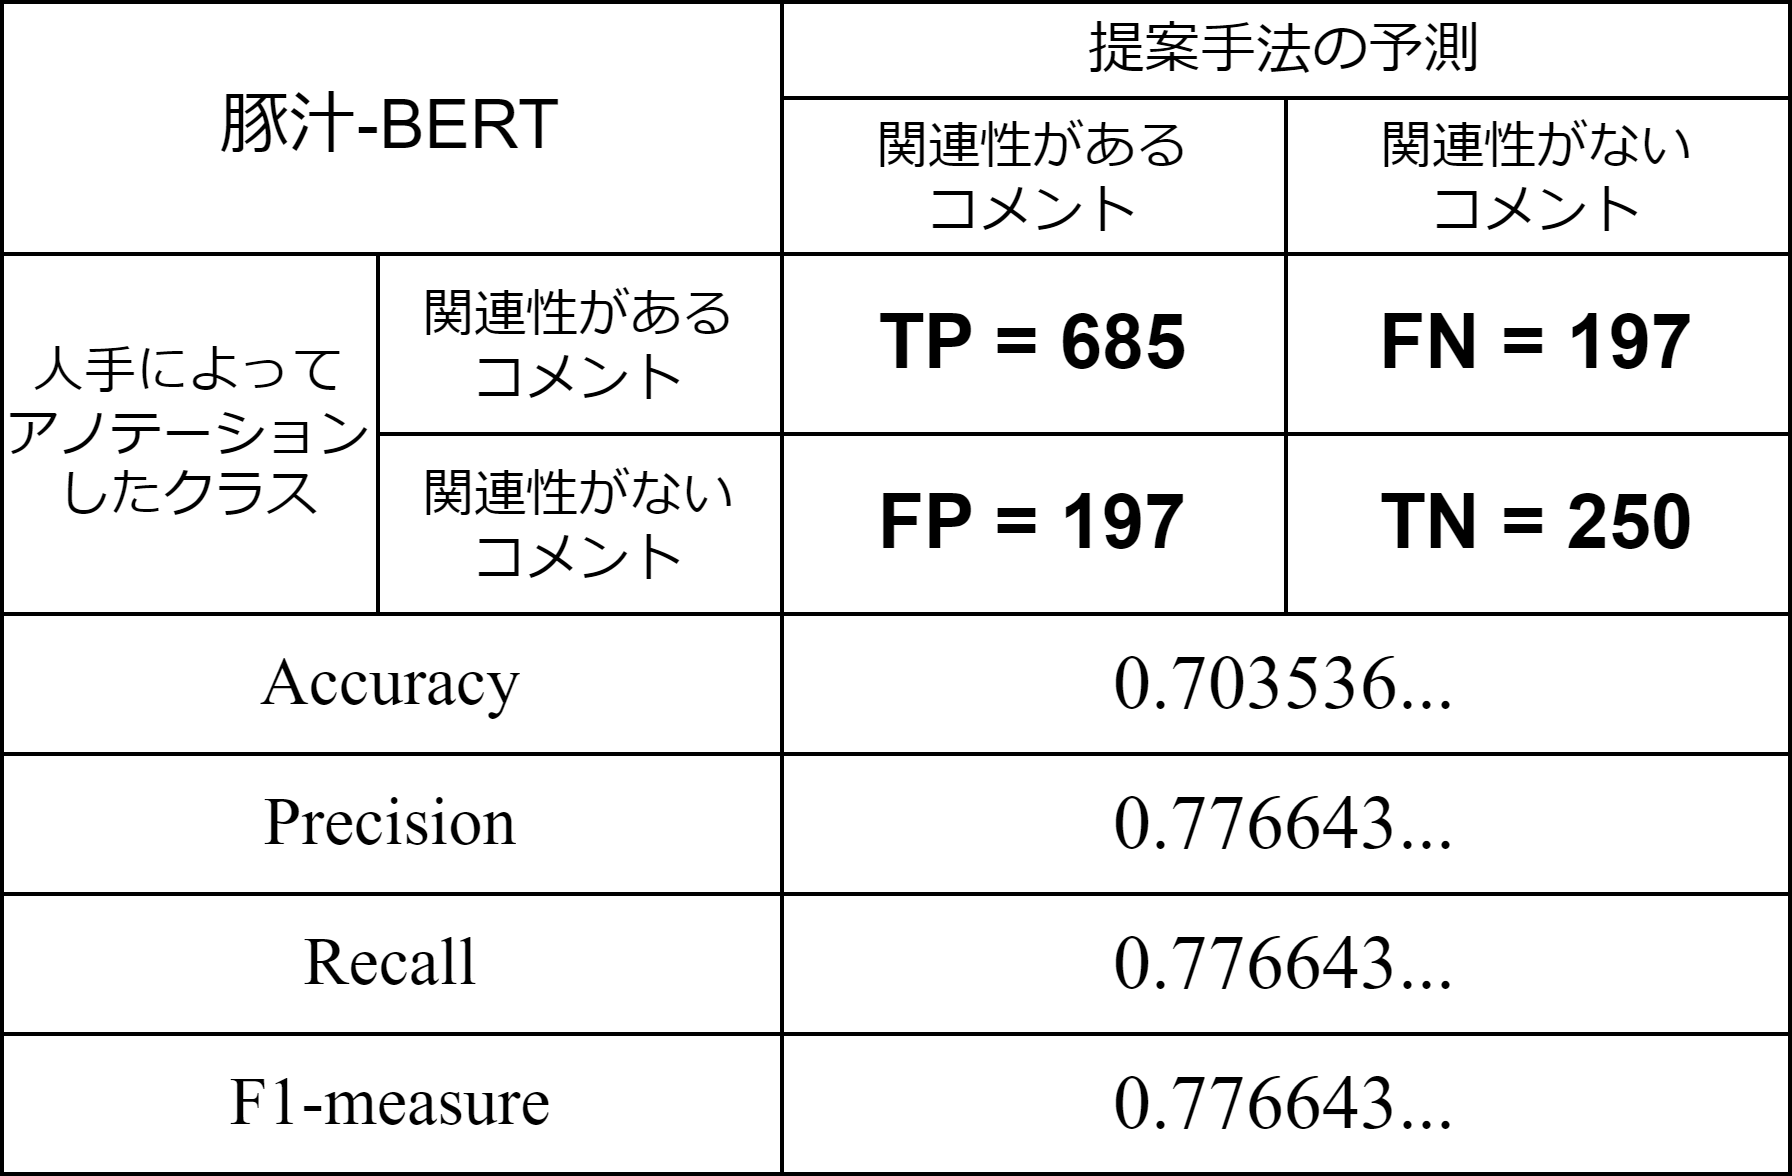
\includegraphics[width = 11.5cm]{images/豚汁images/豚汁Confusion_BERT同件数.drawio.png}
    \label{table:豚汁(BERT)のconfusion同件数}
\end{table}
\vspace{10truept}

表\ref{table:豚汁(TF-IDF)のconfusion同件数}より, TF-IDFを用いて類似度計算をしたデータを用いた場合の全体の正解率は
Accuracy=0.665914であり, 「みそきん」と同様にBERTを用いた手法よりも正解率が下がることが分かった. 
他の指標もBERTを用いた手法より少し低い結果となったが, 「みそきん」の同じ条件の結果と比較すると10\%程度高くなっているため, 
文章生成がより自然で短いことが重要であると考えられる. 
\begin{table}[ht]
    \centering
    \caption{豚汁(TF-IDF)のConfusion Matrix (正解ラベルと同数のラベル付与)}
    \vspace{5truept}

    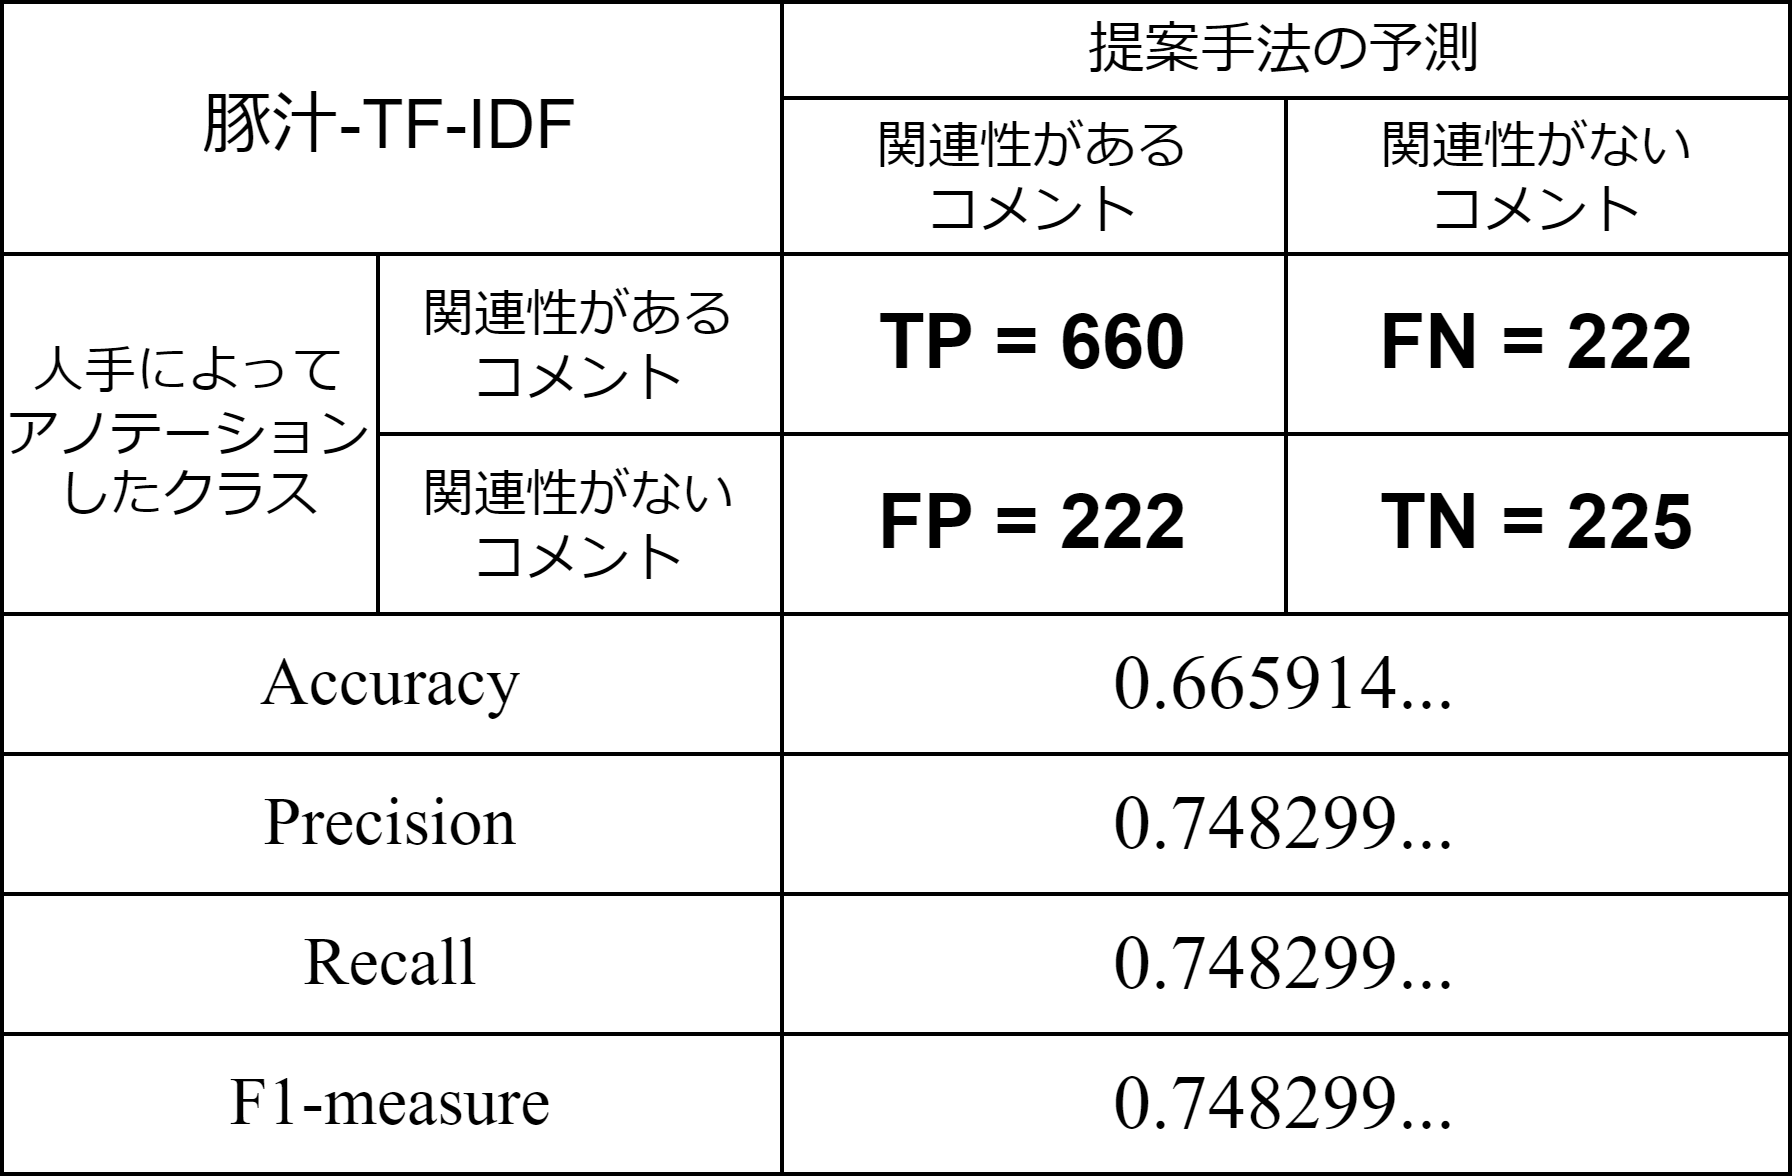
\includegraphics[width = 11.5cm]{images/豚汁images/豚汁Confusion_TF-IDF同件数.drawio.png}
    \label{table:豚汁(TF-IDF)のconfusion同件数}
\end{table}

\newpage
次に, 各類似度計算法によって計算した文章間の類似度の上位25\%, 50\%, 75\%に対して「関連性-高」のラベルを付与して
同様の実験を行った結果を表\ref{table:豚汁BERT閾値}に示す. 
Accuracyを見ると, 閾値をどの値に設定しても全体的な正解率は50\%を超えていて, 閾値を下げたときの正解率の上昇率が「みそきん」の結果
(表\ref{table:みそBERT閾値})よりも高くなっていることが分かる. 
Precisionは閾値を低く設定するにつれて値が低くなるが, 一番低い75\%の場合でも0.76あり, どの閾値に設定した場合でも
提案手法で予測したコメントのうち約7.6割以上が正解していることが分かる. 
閾値を低く設定するにつれてPrecisionが低くなるのは, 誤って「関連性-高」と判断するコメントが増えるからであると考えられる. 
Precisonとは逆にRecallは閾値を低く設定するにつれて値が高くなった. 
これは「関連性-高」と判断するコメントが多くなると, その取りこぼし(「関連性-高」を「関連性-低」と判断する事象)
が少なくなるからであると考えられる. 
Recallの値は閾値25\%のときに約3割であり, 提案手法の性能としては満足できない結果であるが, 
閾値75\%のときは約8.5割で取りこぼしなく関連性があるコメントを抽出できていることが分かる. 
F1-measureを含め, 全ての指標で「みそきん」の結果よりも上回っていることが分かり, 改めて単語抽出と文章生成の結果が重要であると考えられる. 
\begin{table}[ht]
    \centering
    \caption{「関連性-高」の閾値を上位25\%, 50\%, 75\%に設定した結果(BERT)}
    \vspace{5truept}

    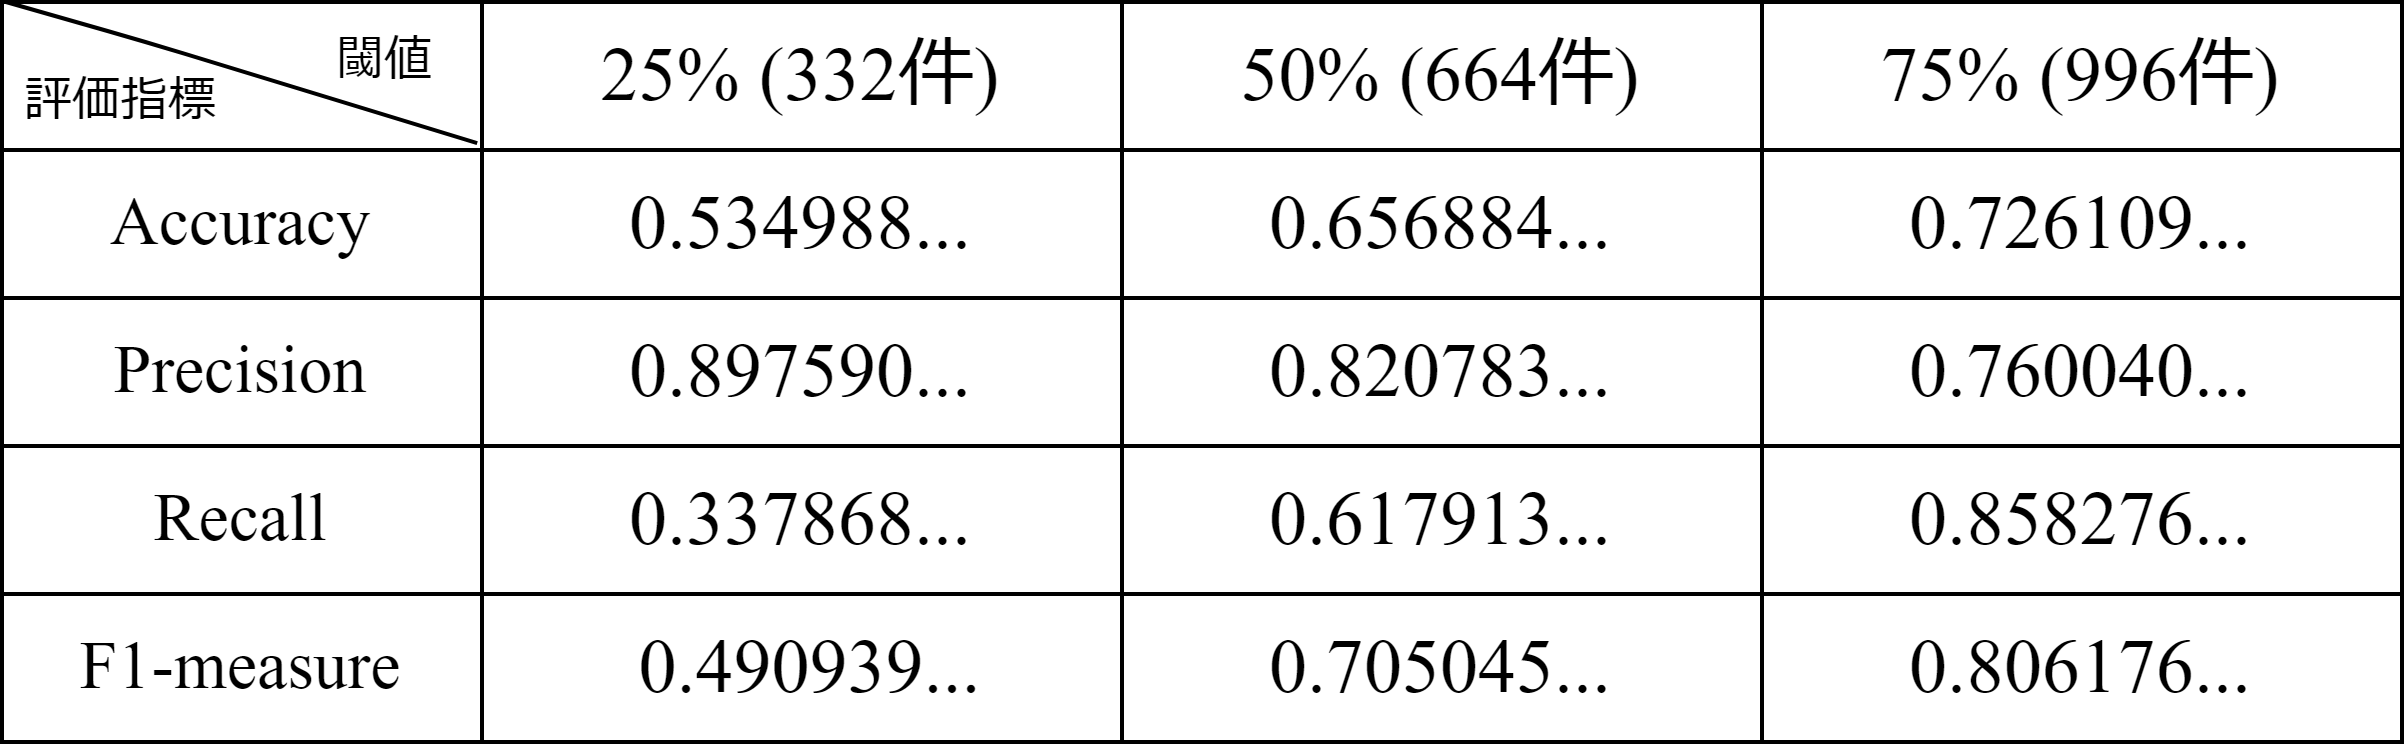
\includegraphics[width = 13.5cm]{images/豚汁images/豚汁BERT閾値.drawio.png}
    \label{table:豚汁BERT閾値}
\end{table}
\vspace{10truept}

次に, TF-IDFを用いた類似度計算したデータに閾値を設定してラベルを付与した結果から計算したConfusion Matrixの各指標を表\ref{table:豚汁TF-IDF閾値}
に示す. BERTでの結果(表\ref{table:豚汁BERT閾値})と比較すると, 「みそきん」と同様に対応している全ての指標が低いことが分かる. 
ここまでの実験でBERTを用いた類似度計算法による結果がTF-IDFを用いた類似度計算による結果を全て上回っているため, 
本提案手法ではBERTによる文章のベクトル化の方が優れているといえる. ただし, 元コメントの文章数や文章の長さによって
結果が変わる可能性があるため, 今後様々な条件を持つコメント集合に対して実験を行う必要がある. 
\begin{table}[ht]
    \centering
    \caption{「関連性-高」の閾値を上位25\%, 50\%, 75\%に設定した結果(TF-IDF)}
    \vspace{5truept}

    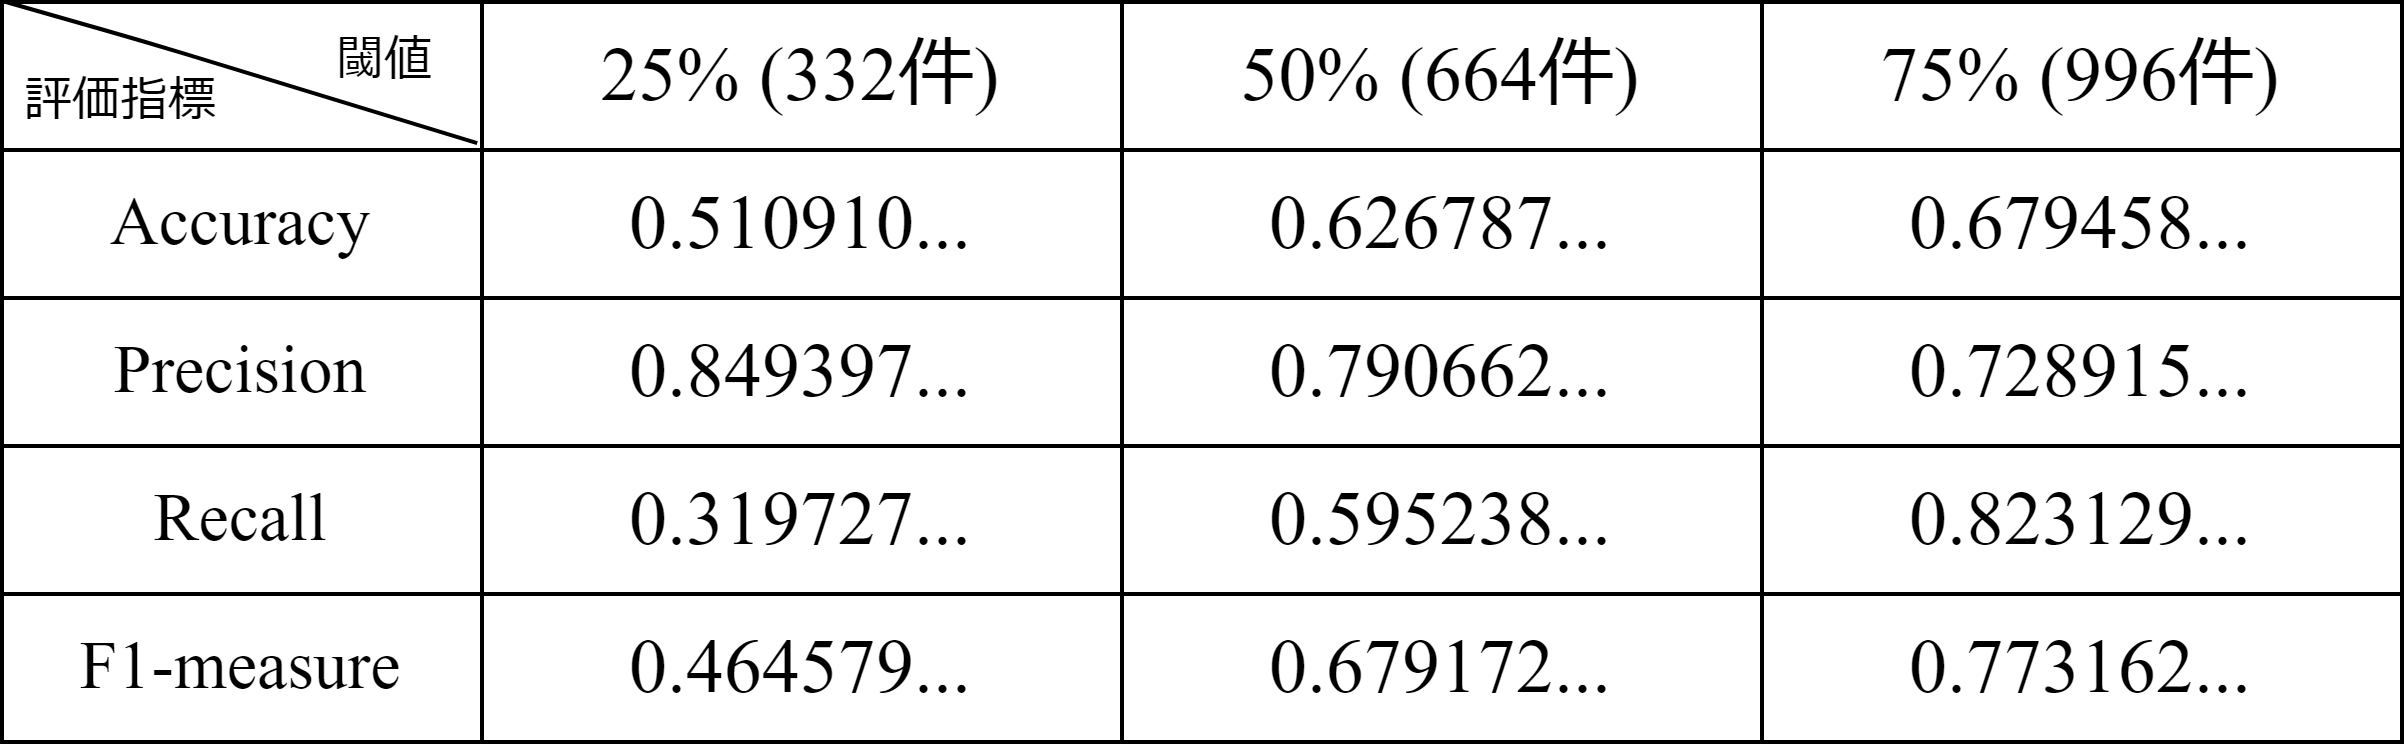
\includegraphics[width = 13.5cm]{images/豚汁images/豚汁TF-IDF閾値.drawio.png}
    \label{table:豚汁TF-IDF閾値}
\end{table}

\newpage
\subsection{極細ボールペンの紹介・比較動画}
次に, 書籍・文房具などを販売している有隣堂の公式YouTubeアカウント「有隣堂しか知らない世界」
から, 極細ボールペンを紹介している動画[9](以下「極細ボールペン」)に対するコメントを用いて実験を行った. 
前節までの実験とは異なり, 企業の公式アカウントであること, 本や文房具を対象としていること
から視聴者の年齢層も比較的高く, 真面目なコメントが多いように感じた. また, コメント総数と平均単語数は
前節までの実験より少なかった. 
以下に詳細な実験条件を示す. 
\vspace{10truept}

\begin{description}
    \item[コメント件数]\mbox{}\\
    抽出したコメントは271件であり, そこから前処理・分かち書きの過程で削除された文章(絵文字のみの文章や一文字のみの文章)
    を除いた270件を用いてBTMで分析した. 人手によるアノテーション, 及び類似度計算に用いるコメントは前処理のみを施した
    コメント270件を用いた. 

    \item[前処理] \mbox{}\\
    前処理の形態素解析の段階では「名詞」と「形容詞」のみを抽出し分かち書きを行った. 
    \item[BTMの各パラメータ]\mbox{}
    \begin{itemize}
        \item トピック数 $T=5$
        \item 単語分布から抽出する出現確率上位の単語数 $n = 10$
        \item 各文章ごとに考慮する単語数 $M=10$
        \item 反復回数 $\textrm{iterations} = 20$
        \item ディリクレ分布のハイパーパラメータ $\alpha, \beta$\\
        他の実験と同じ手法でハイパーパラメータを調整した. 
        「極細ボールペン」では$\alpha = 0.96, \beta = 0.04$で実験を行った. 
    \end{itemize}
\end{description}
\vspace{10truept}

\subsubsection{BTMによって抽出した単語リスト}
上位の条件に従って実験を行い, BTMによって抽出した出力確率上位10単語を表\ref{table:ボールペン単語結果}に示す. 
表\ref{table:ボールペン単語結果}から読み取れる通り, 「ボールペン」, 「ジェットストリーム」, 
「アクロボール」などの商品名が抽出できていることが分かる. 
また, 「ペン先」, 「極細」, 「エッジ」などのボールペンの機能・特徴を表すような単語も抽出できていることが分かる. 
トピックごとに単語を見ると, Topic 2では「ブッコロー」(有隣堂公式アカウントのキャラ), 「岡崎」(商品を紹介している方の名前), 
「面白い」, 「シリーズ」など, このアカウントで商品を紹介しているシリーズに登場しているブッコローと岡崎さんに関するトピックであることが分かる. 
また, Topic 5は「ジェットストリーム」, 「アクロボール」という動画で比較している二つの商品に関する単語が抽出できているため, 
二つの商品の比較のトピックであると考えられる. 
\newpage
\begin{table}[h]
    \caption{BTMで抽出した単語リスト(極細ボールペン)}
    \vspace{5truept}

    \centering
    \begin{tabular}{|c|>{\centering}p{6em}|>{\centering}p{6em}|>{\centering}p{6em}|>{\centering}p{6em}|>{\centering\arraybackslash}p{6em}|}
        \hline
        & Topic 0 & Topic 1 & Topic 2 & Topic 3 & Topic 4\\
        \hline\hline
        1 & ブッコロー & ボールペン & ボールペン & 細い & ジェットストリーム\\
        \hline
        2 & 書き & 極細 & 動画 & 好き & アクロボール\\
        \hline
        3 & 文字 & ジェットストリーム & 愛用 & クリップ & インク\\
        \hline
        4 & 有隣堂 & 細い & シャーペン & アクロ & ボールペン\\
        \hline
        5 & 感動 & ペン & ブッコロー & 最高 & 社長\\
        \hline
        6 & 0階 & 左利き & 岡崎 & 個人的 & ペン先\\
        \hline
        7 & ジェットストリーム & 好き & 気持ち & インク & エッジ\\
        \hline
        8 & デザイン & インク & 面白い & ミリ & 0円\\
        \hline
        9 & ペン先 & パイロット & シリーズ & ジェット & 細く\\
        \hline
        10 & エッジ & 愛用 & キャラ & 大き & トラブル\\
        \hline
    \end{tabular}
    \label{table:ボールペン単語結果}
\end{table}
\vspace{10truept}

\subsubsection{文章生成}
表\ref{table:ボールペン単語結果}に示している単語を使って, ChatGPT(GPT-4)を用いて文章を生成した結果を示す. 
ChatGPTに入力したプロンプトは以下の通りである.  「極細ボールペン」では動画の司会者である「ブッコロー」と商品を紹介している「岡崎」
を人名とする以外は他の実験と同様のプロンプトを入力した. 
\begin{itemize}
    \item 空白区切りで入力する単語を使って文章を生成してください.
    \item 全ての単語を使用してください.
    \item YouTubeのコメントにあるような文章を生成してください.
    \item 可能な限り短い文章を生成してください.
    \item ``ブッコロー'', ``岡崎''は人名として扱ってください.
\end{itemize}
\vspace{10truept}

上記のプロンプトとBTMで得られた各トピックの出現確率上位の単語をChatGPTに入力して文章を生成した結果を表\ref{table:ボールペン生成結果}に示す. 
生成した文章の中には商品を紹介している動画内容と関連性が高い文章もいくつか存在しているが, 動画内容とはかけ離れた文章も生成されていた. 
例えば, Topic 1,3,4の文章はボールペンの内容に関わるような文章が生成されていて, Topic 2はブッコローと岡崎さんが商品を紹介している動画内容
に関連している文章が生成されている. しかし, Topic 0はあまり商品や動画との関連性がない文章が生成されていることが分かる. 
前節までの実験と比べると, 「みそきん」よりも動画や商品との関連性が高い文章が生成されているが, 「豚汁」ほど文章が自然ではないと考えられる. 
\newpage
\begin{table}[h]
    \caption{ChatGPTによる文章生成結果 (極細ボールペン)}
    \vspace{5truept}

    \centering
    \begin{tabular}{|c|l|}
        \hline
        & 生成結果\\
        \hline\hline
        Topic 0 & 
        \begin{tabular}{l}
            ブッコローが有隣堂0階でジェットストリームのペン先のエッジと\\デザインに感動して文字書きしてるの見て、マジで感動したわ。
        \end{tabular}\\
        \hline
        Topic 1 & 
        \begin{tabular}{l}
            極細のボールペンとしてジェットストリームは細いペンが好きな左利きにも\\愛用されていて、インクもパイロットのものが最高!
        \end{tabular}\\
        \hline
        Topic 2 &
        \begin{tabular}{l}
            ブッコローと岡崎が愛用するボールペンとシャーペンの動画シリーズ、\\マジで面白い!キャラの気持ちが伝わってくる。
        \end{tabular}\\
        \hline
        Topic 3 &
        \begin{tabular}{l}
            個人的には、細いインクと大きなクリップが好きで、\\アクロのミリジェットは最高!
        \end{tabular}\\
        \hline
        Topic 4 &
        \begin{tabular}{l}
            ジェットストリームとアクロボールのボールペンは社長も愛用しているけど、ペ\\ン先のエッジが細くてトラブルが0円で解決するなんて、インクの質もさすが!
        \end{tabular}\\
        \hline
    \end{tabular}
    \label{table:ボールペン生成結果}
\end{table}
\vspace{10truept}

\subsubsection{二種の類似度計算法による結果}
ChatGPT(GPT-4)で生成した文章と, 前処理を施した元のYouTubeのコメントとの文章間の類似度を計算した結果を述べる. 
他の実験と同様にBERTとTF-IDFによる文章のベクトル化を用いてCos類似度を計算し, 二つの手法がどのような特徴を
持っているか, また文章数や平均単語数が少ない場合にどちらが優位なのかを考察する. 
図\ref{fig:ボールペン類似度BERT}, \ref{fig:ボールペン類似度TF-IDF}は各類似度計算法によって算出した文章間の類似度をグラフ化したものである. 
「みそきん」の結果と同様に, BERTを用いた手法ではほとんどのコメントが0.8\sim0.96の値を取っている. 
しかし, TF-IDFを用いた手法では「みそきん」や「豚汁」と比べて0\sim0.7の値を持つコメントの数が少ないことが図\ref{fig:ボールペン類似度TF-IDF}
から分かった. 
これは「極細ボールペン」の元コメントが他の動画に比べて質が高い(意味の通る文章である)ことが多いからであると考えられ, 
それは他の動画とは異なり企業の公式アカウントに対するコメントであることに起因すると考えられる. 
表\ref{table:ボールペン類似度結果BERT}, 
\ref{table:ボールペン類似度結果TF-IDF}はそれぞれの類似度計算法の結果の一例であり, 後に人手でアノテーションする際には
「関連性-高」と判断されるコメントである. 
表\ref{table:ボールペン類似度結果TF-IDF}では長さが短い文章のときに類似度が低くなってしまっているが, 
同じコメントに対して表\ref{table:ボールペン類似度結果BERT}では類似度が高く算出されている. 
しかし, 他の実験に比べてTF-IDFを用いた手法でも低い類似度を示すコメントが少ないため, 
BERTの優位性が顕著に表れているとは言えないと考えられる. 

\newpage
\begin{figure}[ht]
    \centering
    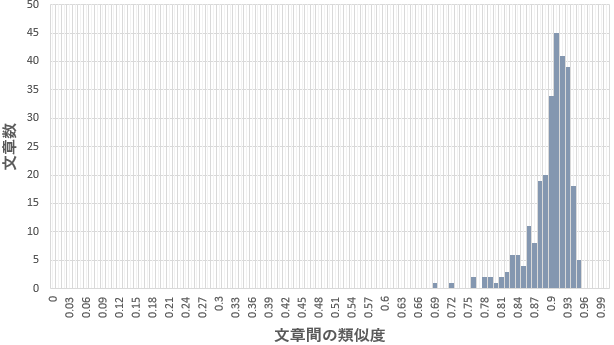
\includegraphics[width = 13.1cm]{images/ボールペンimages/BERT類似度.png}
    \caption{BERTによる類似度計算結果}
    \label{fig:ボールペン類似度BERT}
\end{figure}
\vspace{30truept}

\begin{table}[ht]
    \caption{BERTによる類似度計算結果の一例}
    \vspace{5truept}

    \centering
    \begin{tabular}{|r|l|}
        \hline
        類似度結果 & 前処理済みの元コメント\\
        \hline\hline
        0.948193431 & 
        \begin{tabular}{l}
            その昔ハイテックcが出始めた頃自分の筆圧の強さでダメにして以来極細\\ボールペンには抵抗がありましたジェットストリームの0mmが限界かなぁ\\また書けなくしていまいそうで\\
        \end{tabular}\\
        \hline
        0.932215512 & 
        \begin{tabular}{l}
            極細ならシグマとハイテックも入れて欲しかった\\
        \end{tabular}\\
        \hline
        0.921288013 & 
        \begin{tabular}{l}
            0年近く前からパイロットの0のボールペン出てるけどそっから進化は\\してないんだなぁ\\
        \end{tabular}\\
        \hline
        0.910937369 & 
        \begin{tabular}{l}
            0mmは細かいとこ書くのに重宝したな特にセンター試験の願書\\に貼る検定料受付証明書とかクッソちっちゃい欄に住所と氏名\\書かなきゃならんからわざわざ買いに行ったレベル\\
        \end{tabular}\\
        \hline
        0.90612942 & 
        \begin{tabular}{l}
            出来れば作図用0がほしい\\
        \end{tabular}\\
        \hline
        0.892260015 & 
        \begin{tabular}{l}
            岡崎さんがほんとに可愛いらしくてファンになりました\\やけにインテリなチンピラのようなブッコローに負けないで\\今日まで頑張ってくれてありがとうございます\\
        \end{tabular}\\
        \hline
        0.824225068 & 
        \begin{tabular}{l}
            ブッコロー面白すぎ\\
        \end{tabular}\\
        \hline
    \end{tabular}
    \label{table:ボールペン類似度結果BERT}
\end{table}

\newpage
\begin{figure}[ht]
    \centering
    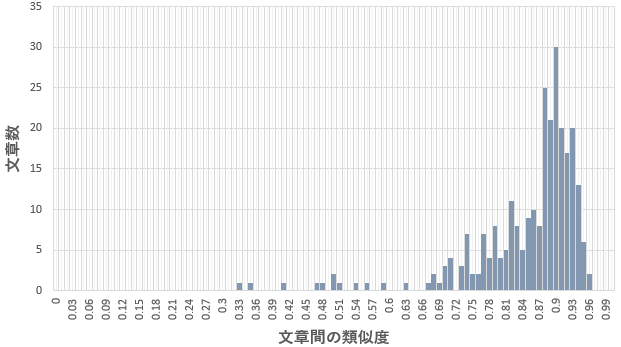
\includegraphics[width = 13cm]{images/ボールペンimages/TF-IDF類似度.png}
    \caption{TF-IDFによる類似度計算結果}
    \label{fig:ボールペン類似度TF-IDF}
\end{figure}
\vspace{30truept}

\begin{table}[ht]
    \caption{TF-IDFによる類似度計算結果の一例}
    \vspace{5truept}

    \centering
    \begin{tabular}{|r|l|}
        \hline
        類似度結果 & 前処理済みの元コメント\\
        \hline\hline
        0.935953529 & 
        \begin{tabular}{l}
            その昔ハイテックcが出始めた頃自分の筆圧の強さでダメにして以来極細\\ボールペンには抵抗がありましたジェットストリームの0mmが限界かなぁ\\また書けなくしていまいそうで\\
        \end{tabular}\\
        \hline
        0.93580221 & 
        \begin{tabular}{l}
            0年近く前からパイロットの0のボールペン出てるけどそっから進化は\\してないんだなぁ\\
        \end{tabular}\\
        \hline
        0.906806296 & 
        \begin{tabular}{l}
            岡崎さんがほんとに可愛いらしくてファンになりました\\やけにインテリなチンピラのようなブッコローに負けないで\\今日まで頑張ってくれてありがとうございます\\
        \end{tabular}\\
        \hline
        0.887666573 & 
        \begin{tabular}{l}
            0mmは細かいとこ書くのに重宝したな特にセンター試験の願書\\に貼る検定料受付証明書とかクッソちっちゃい欄に住所と氏名\\書かなきゃならんからわざわざ買いに行ったレベル\\
        \end{tabular}\\
        \hline
        0.846231257 & 
        \begin{tabular}{l}
            極細ならシグマとハイテックも入れて欲しかった\\
        \end{tabular}\\
        \hline
        0.829074881 & 
        \begin{tabular}{l}
            出来れば作図用0がほしい\\
        \end{tabular}\\
        \hline
        0.537144551 & 
        \begin{tabular}{l}
            ブッコロー面白すぎ\\
        \end{tabular}\\
        \hline
    \end{tabular}
    \label{table:ボールペン類似度結果TF-IDF}
\end{table}
\newpage
\subsubsection{提案手法の精度検証結果}
文章間の類似度を計算し, その値が高いコメントを「商品(極細ボールペン)との関連性がある」と判断するという仮説を検証するため, 
人手でアノテーションして正解ラベルを付与したデータと比較して分析を行う. 
「極細ボールペン」のコメントに対するアノテーションは以下の基準で行った. アノテーションを行った結果, 「関連性-高」のラベルが付与された
コメントが154件, 「関連性-低」のラベルが付与されたコメントが116件であった. 
\vspace{10truept}

\begin{description}
    \item[関連性-高]\mbox{}
    \begin{itemize}
        \item 紹介している極細ボールペンに直接関係するコメント(例:デザイン, 細さ, 値段など)
        \item 実際に使用した感想(例:書き心地, 握りやすさなど)
        \item 他のボールペンとの比較(例:値段が高い, 使いやすさなど)
    \end{itemize}
    \item[関連性-低] \mbox{}
    \begin{itemize}
        \item ボールペンには関係ないが動画には関係しているコメント(例:このシリーズ面白いなど)
        \item 商品を紹介している人に対するコメント(例:ブッコロー(キャラ)についてなど)
        \item その他全く関係ないコメント
    \end{itemize}
\end{description}
\vspace{10truept}

人手でアノテーションし正解ラベルを付与したデータと, 提案手法によって類似度を計算したコメントを比較し, 
提案手法の精度, 及び仮説の検証を行う. 
提案手法では類似度を計算しただけであり, 商品との関連性が高いと言える閾値は設定されていない. 
そのため, 類似度上位のコメントに対して, 人手で「関連性-高」のラベルを付与した数と同じ数のコメントだけ
「関連性-高」のラベルを付与する. 
それ以下の類似度のコメントには「関連性-低」のラベルを付与する. 
「極細ボールペン」の場合, 正解ラベルは「関連性-高」が154件, 「関連性-低」が116件であり, 同じ数だけラベル付けした
データを用いて, 二値分類のConfusion Matrixを計算する. 
また, 「みそきん」と同様に類似度上位25\%, 50\%, 75\%を閾値として「関連性-高」のラベル
を付与したデータを作成し, 同様にConfusion Matrixを計算することで提案手法の精度をより深く考察する. 
\vspace{20truept}

まず初めに, 人手の正解ラベルと同数のラベルを付与した結果について述べる. 
BERTを用いて類似度計算したデータから求めたConfusion Matrixを表\ref{table:ボールペン(BERT)のconfusion同件数}に, 
TF-IDFを用いて類似度計算したデータから求めたConfusion Matrixを表\ref{table:ボールペン(TF-IDF)のconfusion同件数}に示す. 
表\ref{table:ボールペン(BERT)のconfusion同件数}より, 「極細ボールペン」に対する提案手法の全体的な正解率はAccuracy=0.688888であり, 
「みそきん」よりも正解率が高く, 「豚汁」より低いことが分かった. 
また, Precision, Recall, F1-measure=0.727272であり, 同様に「みそきん」
よりも高い精度でコメントを分類できていることが分かった. Precisionが0.727272であることから, 
提案手法で予測したコメントのうち約7.3割が人手で関連性があると判断したコメントであることが分かり, 提案手法に有用性があると判断することができると思われる. 
Recallも同様に0.727272であり, 人手で関連性があると判断したコメントのうち約7.3割が提案手法で関連性があると予測されているため, 
他のユーザーにとって有益なコメントの取りこぼしが少ないといえる. 
\newpage
\begin{table}[ht]
    \centering
    \caption{ボールペン(BERT)のConfusion Matrix (正解ラベルと同数のラベル付与)}
    \vspace{5truept}

    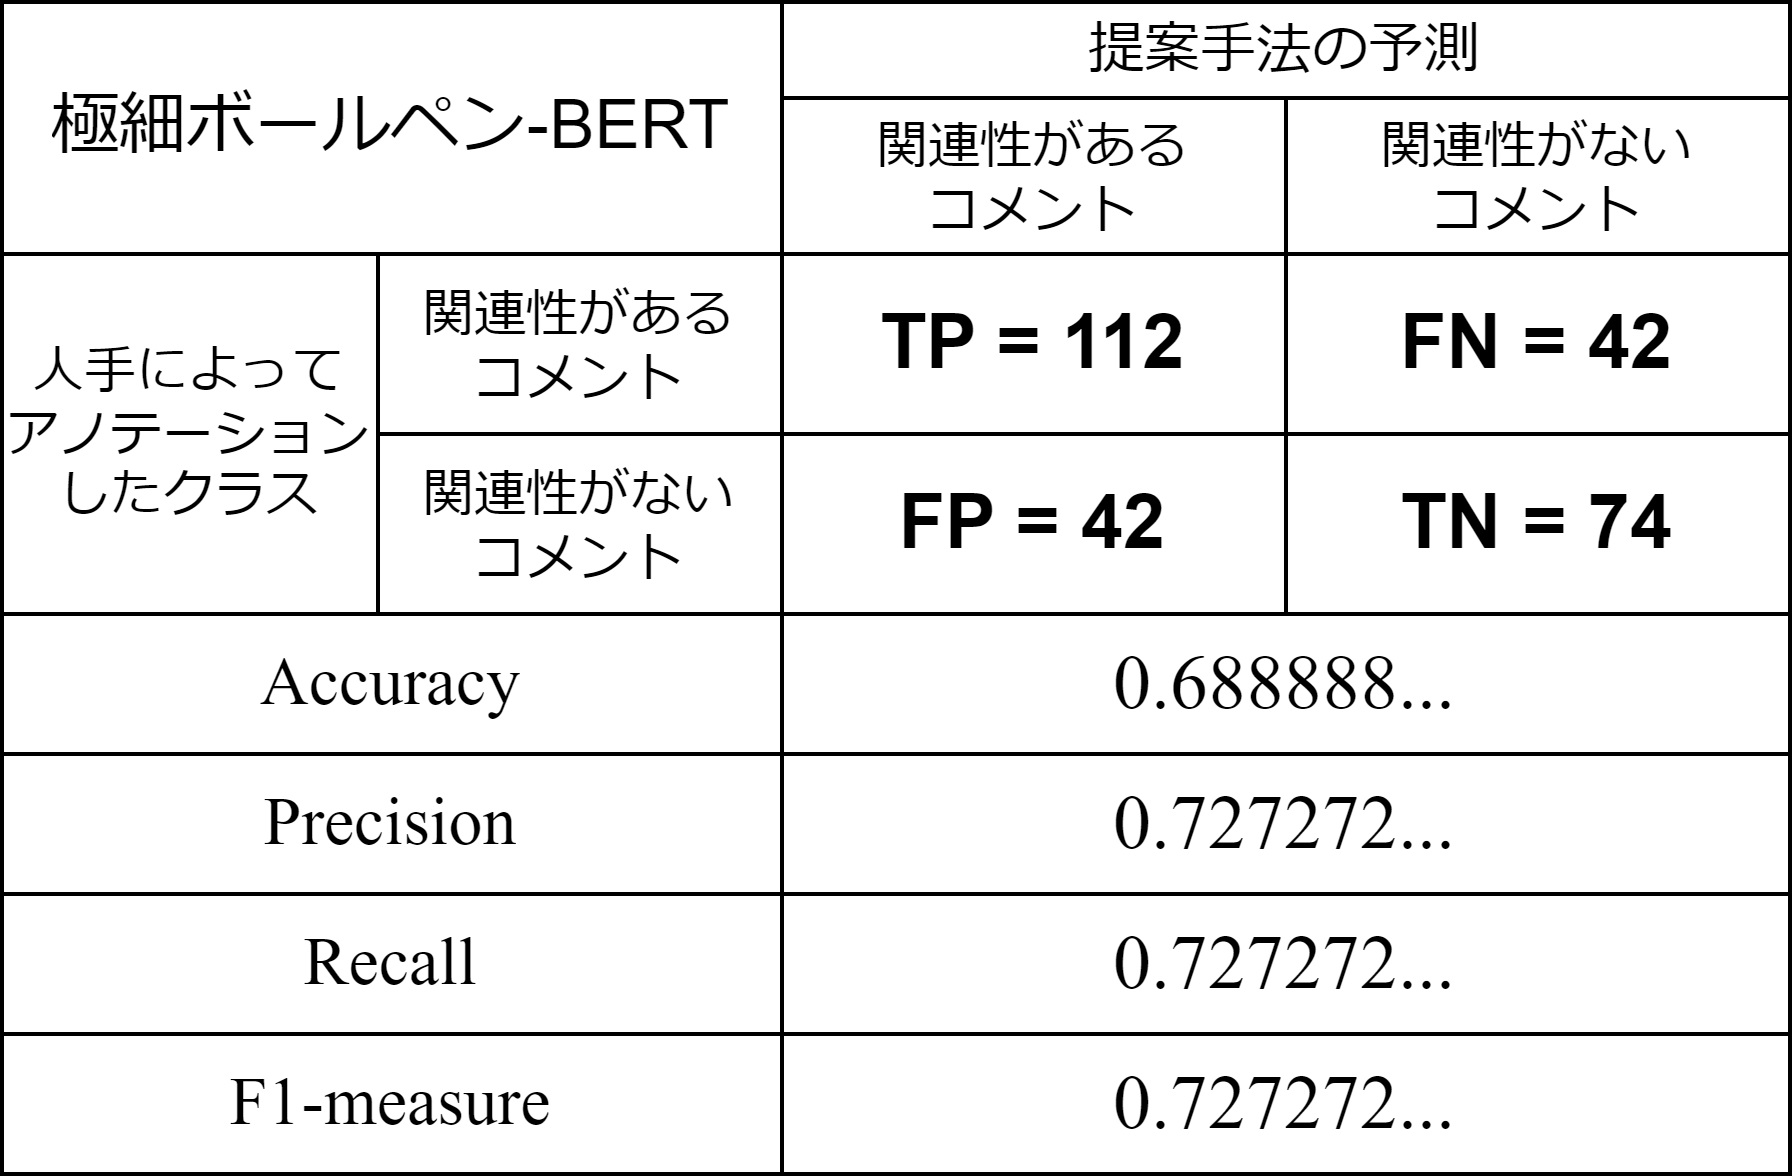
\includegraphics[width = 11.5cm]{images/ボールペンimages/BERT同件数.drawio.png}
    \label{table:ボールペン(BERT)のconfusion同件数}
\end{table}
\vspace{30truept}

表\ref{table:ボールペン(TF-IDF)のconfusion同件数}より, TF-IDFを用いて類似度計算をしたデータを用いた場合の全体の正解率は
Accuracy=0.733333であり, 他の実験とは異なりBERTのAccuracyよりも高くなっていることが分かった. 
また, 他の指標も同様にBERTの結果よりも高く, 「極細ボールペン」ではTF-IDFを用いた類似度計算の方が提案手法に適していると
言える結果となった. 
\begin{table}[ht]
    \centering
    \caption{ボールペン(TF-IDF)のConfusion Matrix (正解ラベルと同数のラベル付与)}
    \vspace{5truept}

    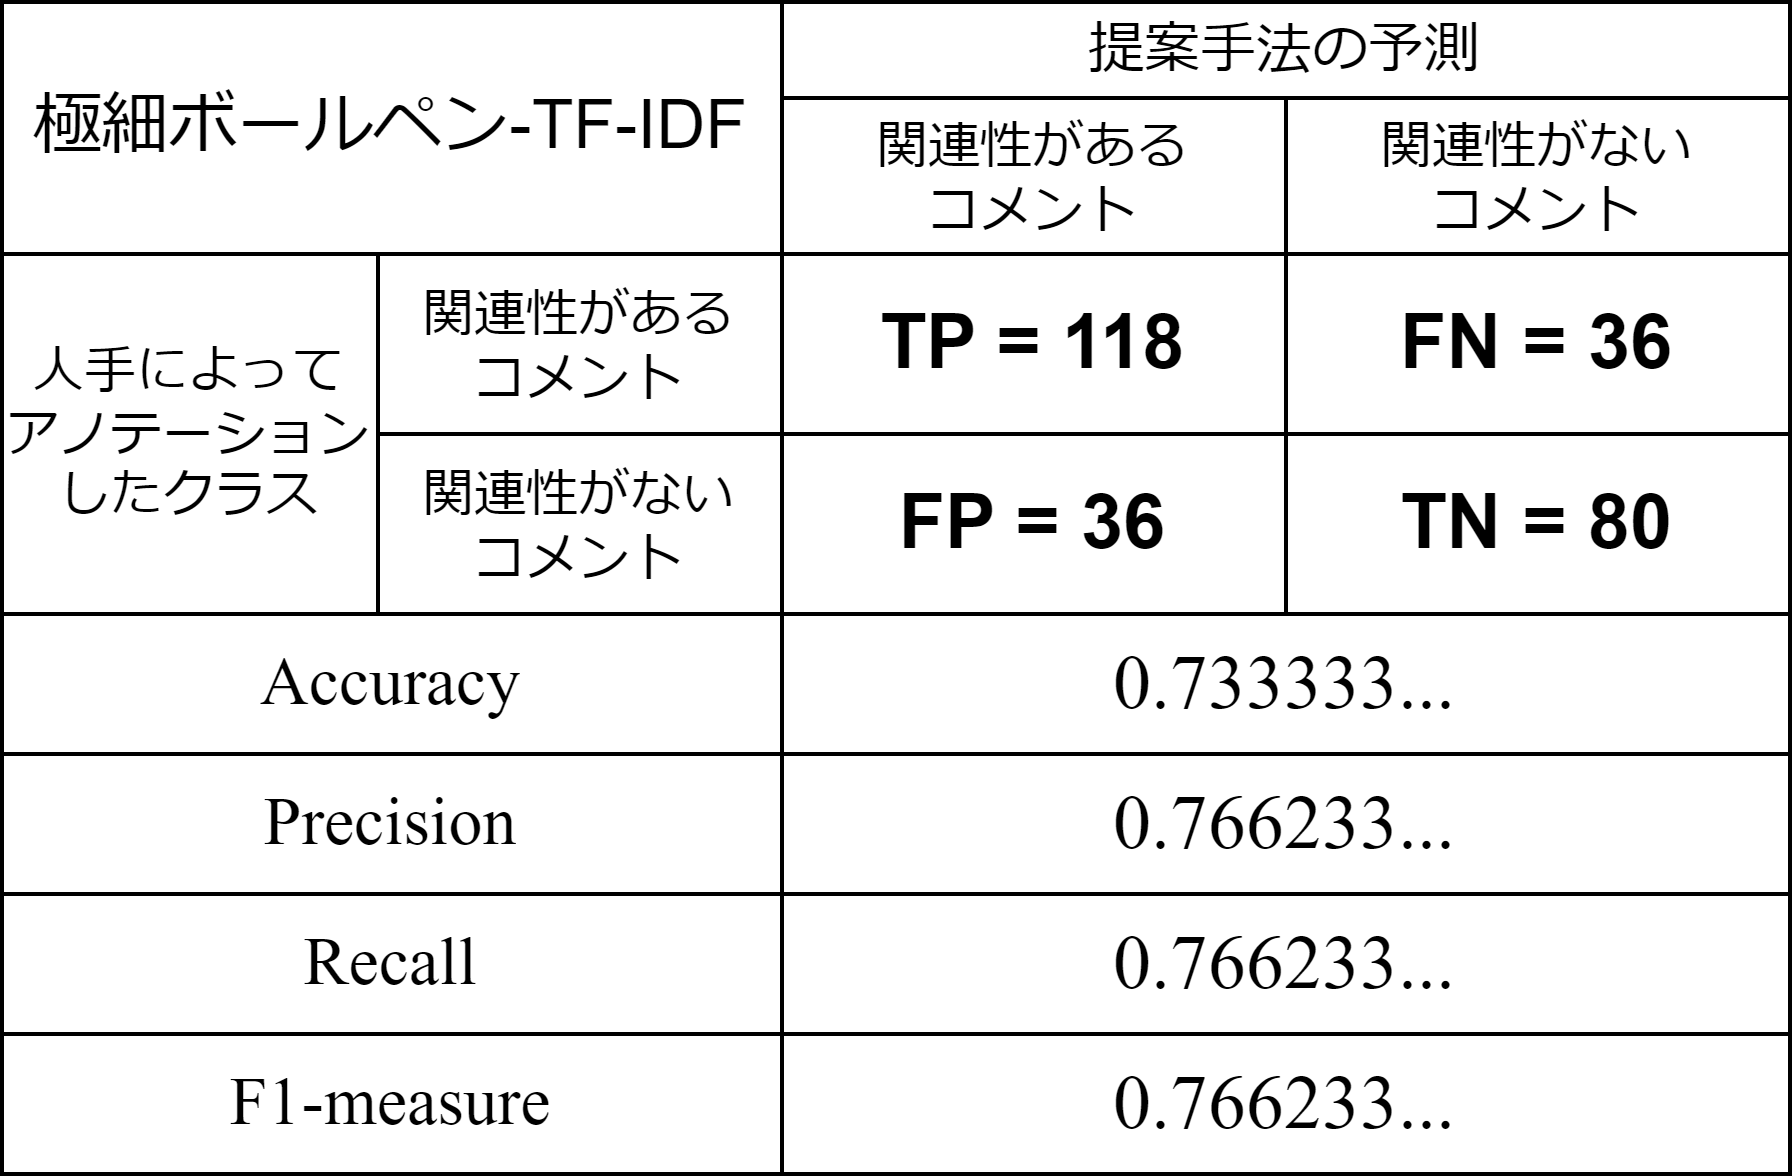
\includegraphics[width = 11.5cm]{images/ボールペンimages/TF-IDF同件数.drawio.png}
    \label{table:ボールペン(TF-IDF)のconfusion同件数}
\end{table}

次に, 各類似度計算法によって計算した文章間の類似度の上位25\%, 50\%, 75\%に対して「関連性-高」のラベルを付与して
同様の実験を行った結果を表\ref{table:ボールペンBERT閾値}に示す. 
Accuracyを見ると, 閾値をどの値に設定しても全体的な正解率は50\%を超えていて, 閾値を下げたときの正解率の上昇率が「みそきん」の結果
(表\ref{table:みそBERT閾値})よりも高くなっていることが分かる. 
\newpage
\noindent また, 「豚汁」の結果と比較すると閾値25\%, 50\%時点では精度が高くなっているが, 75\%では今回の結果の方が低くなっていることが分かる. 
Precisionは閾値を低く設定するにつれて値が低くなるが, 一番低い75\%の場合でも0.68あり, どの閾値に設定した場合でも
提案手法で予測したコメントのうち約6.8割以上が正解していることが分かる. 
閾値を低く設定するにつれてPrecisionが低くなるのは, 誤って「関連性-高」と判断するコメントが増えるからであると考えられる. 
Precisonとは逆にRecallは閾値を低く設定するにつれて値が高くなった. 
これは「関連性-高」と判断するコメントが多くなると, その取りこぼし(「関連性-高」を「関連性-低」と判断する事象)
が少なくなるからであると考えられる. 
Recallの値は閾値25\%のときに約3.5割であり, 提案手法の性能としては満足できない結果であるが, 
閾値75\%のときは約9割で取りこぼしなく関連性があるコメントを抽出できていることが分かる. 
全体の指標を他の実験と比較すると, 「みそきん」よりは全ての指標で良い精度が確認でき, 「豚汁」と比べるとRecallがどの閾値でも上回っている
ことが分かった. 
\begin{table}[ht]
    \centering
    \caption{「関連性-高」の閾値を上位25\%, 50\%, 75\%に設定した結果(BERT)}
    \vspace{5truept}

    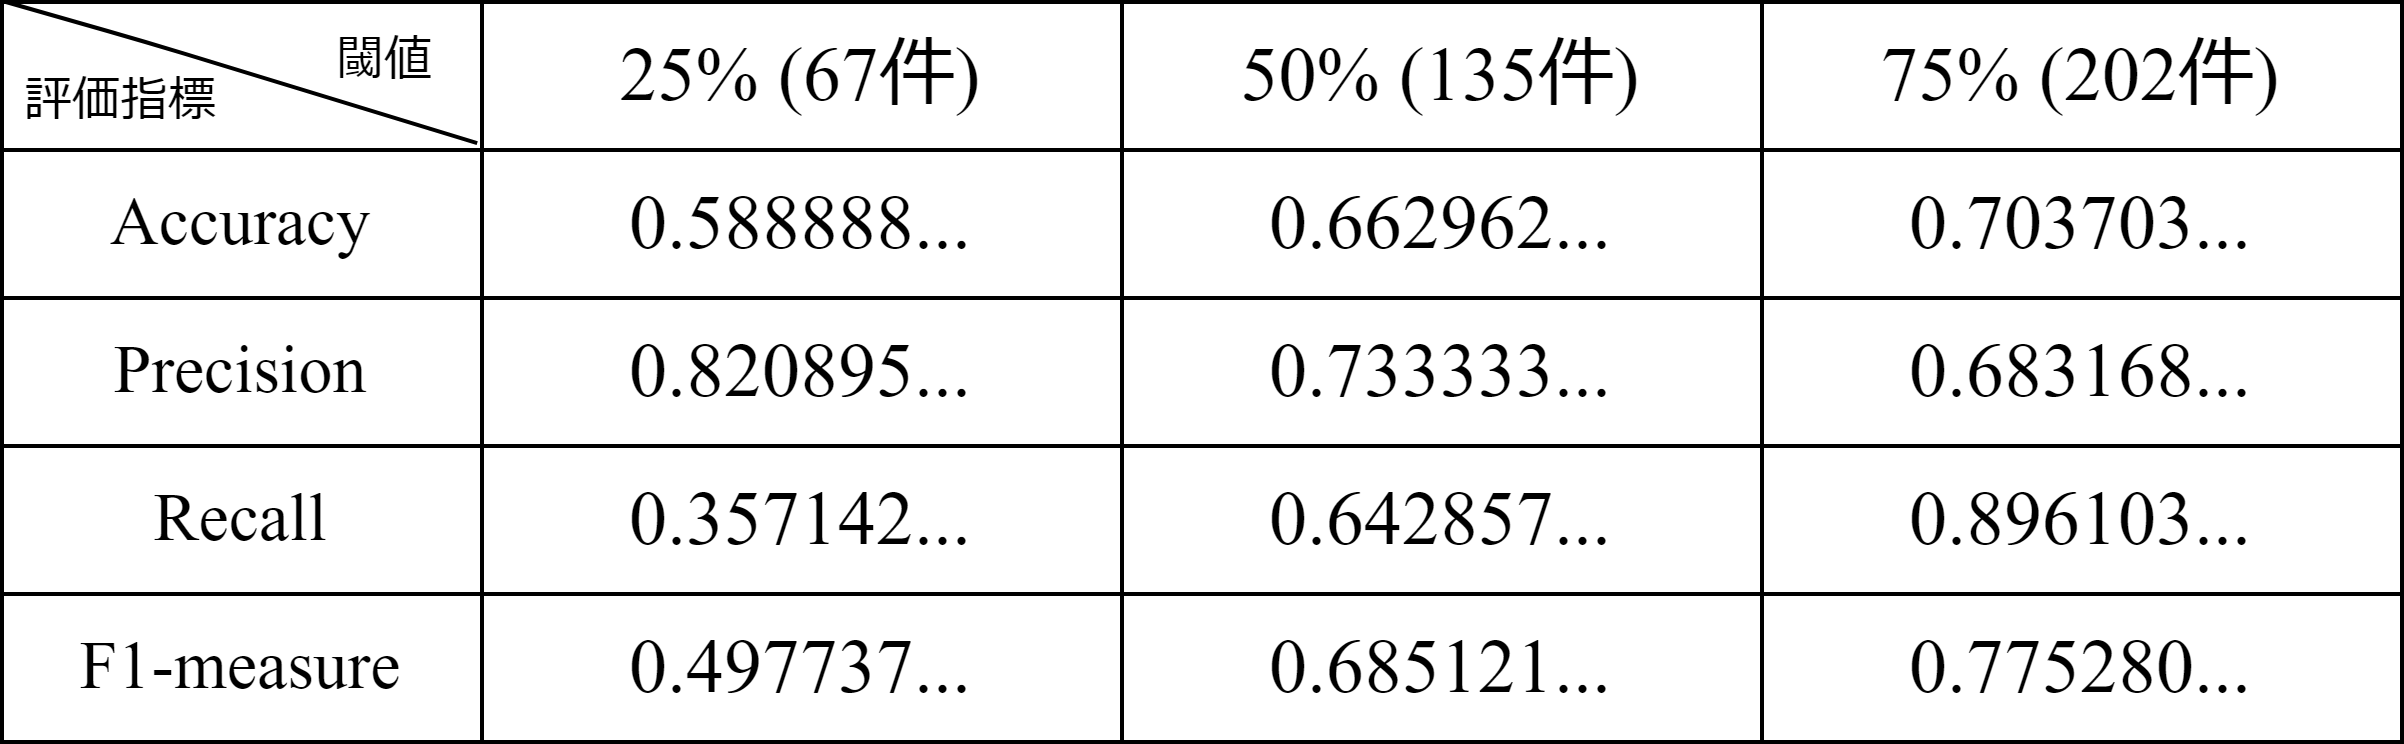
\includegraphics[width = 13.5cm]{images/ボールペンimages/BERT閾値.drawio.png}
    \label{table:ボールペンBERT閾値}
\end{table}
\vspace{10truept}

次に, TF-IDFを用いた類似度計算したデータに閾値を設定してラベルを付与した結果から計算した
Confusion Matrixの各指標を表\ref{table:ボールペンTF-IDF閾値}
に示す. 
BERTでの結果(表\ref{table:ボールペンBERT閾値})と比較すると, 
これまでの実験とは異なり, 全ての指標・閾値でTF-IDFの方が優れた結果を示していることが分かった.  
これはコメント数や平均単語数, コメントの質などに影響されて異なる結果が示されていると考えられる. 
「極細ボールペン」ではコメント数が270件と少ないことから, TF-IDFによる特徴量抽出のフェーズにおいて, 
各文書における単語の重要度が際立ち, より正確な文章の埋め込みを行えていると考えられる. 
また, 企業の公式アカウントに対するコメントであること, コメント数が少ないことから, 質の高いコメントの割合が
他の実験と比べて多いことが影響していると考えられる. 
\begin{table}[ht]
    \centering
    \caption{「関連性-高」の閾値を上位25\%, 50\%, 75\%に設定した結果(TF-IDF)}
    \vspace{5truept}

    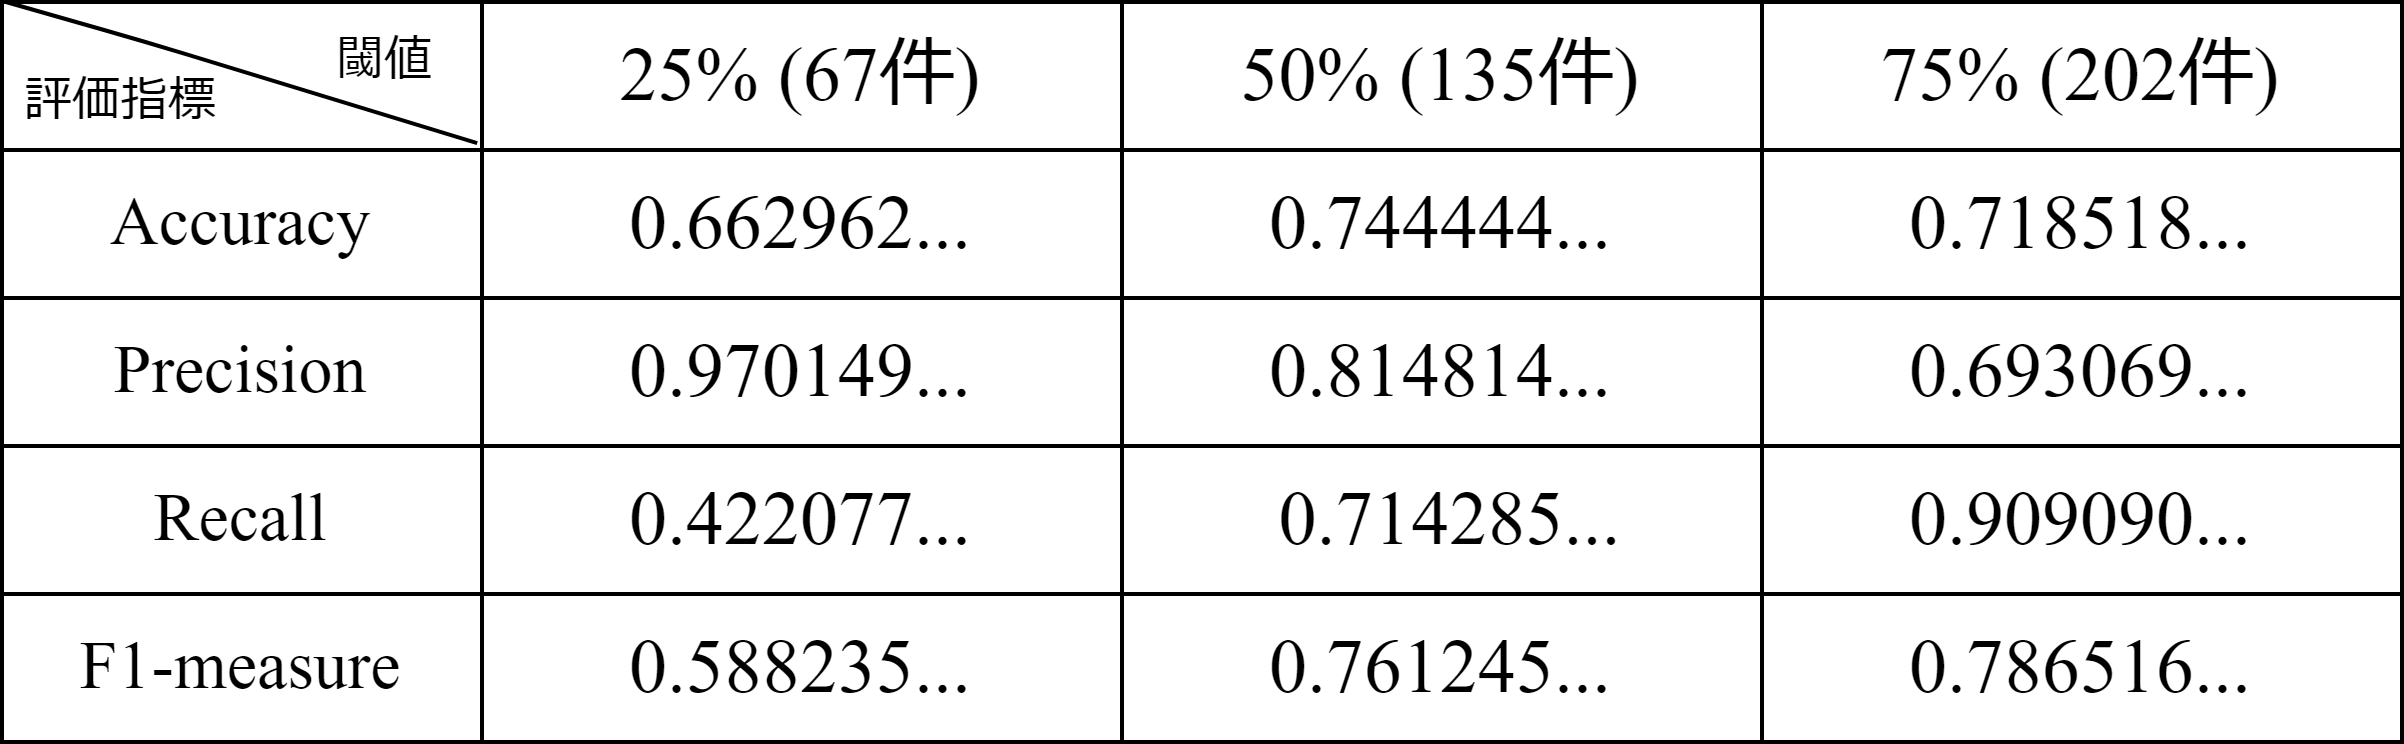
\includegraphics[width = 13.5cm]{images/ボールペンimages/TF-IDF閾値.drawio.png}
    \label{table:ボールペンTF-IDF閾値}
\end{table}

\newpage
\section{考察}
6節で述べてきた実験結果より, 提案手法の有用性, 及び仮説の検証結果についての考察をまとめる. 
\subsection{BTMの優位性についての考察}
BTMによるトピックの推定とそのトピックの単語分布から出現確率上位の単語を抽出した結果より, BTMを用いることで
YouTubeのような一文の長さが比較的短い文書集合からでもトピックを適切に推定できることが分かった. 
また, 動画の主題(宣伝している商品やサービス,レシピ)に関連する単語を主に抽出していたため, 
YouTubeのコメント集合から動画の主題を推定する手法としてトピックモデルが有用であると考えられる. 
従来のトピックモデルであるLDAによる実験では, BTMに比べて抽出する単語に記号や数字が含まれていたり, 
抽出した単語の被りが多いことから文章生成の質が落ちていると思われる. 
その結果全ての指標でBTMより少し劣っていることが分かったが, BTMの優位性を明らかにするには
一文の長さが極端に短いコメントを多く含む動画や, 文章数が多い, または少ない場合で実験を行う必要があると考えられる. 

\subsection{文章生成に関する仮説の検証}
BTMによってトピックの出現確率上位の単語を抽出し, それらの単語を用いてChatGPT(GPT-4)で文章生成を行った. 
ここで生成した文章は, BTMによってコメント集合, つまり対象のYouTubeの動画に関するトピックに対して代表的な文章である
という仮説を立てている. この仮説に妥当性がある場合, 生成した文章と元のYouTubeのコメントとの文章間の類似度
を計算したとき商品・サービスとの関連性が高いコメントの類似度が高く算出されると考えられる. 
この仮説を検証するため, 人手でアノテーションしたデータと類似度計算したデータを比較した. 
その結果, 対象の動画によってぶれは生じるがAccuracyが0.6\sim0.7程度, Precisionが0.7\sim0.8程度となり, 
類似度を計算した結果に妥当性があるといえる結果となった. 
このことから, BTMによって抽出した単語を用いてChatGPTにより生成した文章は対象の動画のトピックに対して代表的な文章である
という仮説の妥当性が示されていると考えられる. 

\subsection{類似度計算方法の考察}
BERTを用いて文章をベクトル化しCos類似度を計算する手法と, TF-IDFを用いて文章をベクトル化しCos類似度を計算する手法
の二種類の類似度計算法を比較し, どちらが本研究の提案手法として優れているかを考察する. 
「みそきん」, 「豚汁」の類似度計算の結果より, 商品との関連性が高いコメントの類似度がBERTを用いた手法では適切に高い値を示していたのに対し, 
TF-IDFでは低い値を示しているコメントが多く存在した. 特に文章の長さが短い場合に適切な値をとらないコメントが多いと思われる. 
また, Confusion Matrixより算出した各指標から, BERTを用いた手法の方がTF-IDFを用いた手法よりもAccuracyやPrecision
が高い結果となった. このことから, 本研究の提案手法で用いる類似度計算法としてはBERTを用いた手法の方が優れているといえる. 
しかし, 「極細ボールペン」の結果ではBERTよりTF-IDFの方が精度が良い結果となったため, 全ての動画に対してBERTが優位であるとは言えないと考えられる. 
例えば, 一文の長さが極端に短いコメントが多い場合や対象の動画に対するコメントの傾向, 例えば気軽に投稿できる雰囲気であるかよく考えられた文章の割合
が多いコメント欄であるかどうかにより結果が異なる可能性があるため, 様々な条件下での実験を行いBERTの優位性を明らかにする必要があると考えられる. 

\subsection{提案手法の有用性についての考察}
YouTube上で自社製品やサービスを宣伝している動画に対するコメントのうち, 対象の商品・サービスに関連しているコメント
を抽出する提案手法の有用性, 実用性について考察する. 
各実験のConfusion Matrixより算出された評価指標から, 提案手法の全体的な正解率(Accuracy)は約6割\sim7割程度であることが分かり, 
関連性の有無の分類をある程度行えているといえる. 
しかし, Accuracyはラベルの偏りが著しい場合に適切な評価を行えないため, ラベルの偏りが少ないコメント集合を持つ動画に対してのみ
有効な指標であると考えられる. 
Precisionは予測モデルがPositiveだと判断した事象のうち正解がPositiveである事象の割合であり, 
本研究においては提案手法によって「関連性-高」と判断されたコメントのうち人手で「関連性-高」と判断できるコメントの割合である. 
各実験結果よりPrecisionは0.7\sim0.8程度の値を示した. このことから, 提案手法によって関連性が高いと判断したコメントのうち
約7割\sim8割が正解しているため, 提案手法の有用性が示されていると考えられる. また, Recallは人手で関連性ありと判断したコメント
が提案手法によってどれくらい関連性ありと判断されるかの指標であり, 他のユーザーにとって有益な情報をどれだけ取りこぼさないか
という意味でもある. 関連性があると判断する閾値を人手のラベルと同数に設定した場合, RecallはPrecisonと同じ値になるため, 
提案手法によってYouTubeの元コメントから有益なコメントを抽出できることも示されていると考えられる. 
最後に, 閾値を上位25\%, 50\%, 75\%に設定した場合の結果について考察する. 
人手のラベルと同数に設定した結果と比較すると, 75\%に設定したときにAccuracy, 及びF1-measureが高くなった. 
しかし, 提案手法の精度を検証する際に一番適切なPrecisionに関しては人手のラベルと同数に設定したときの方が高いため, 
本研究の目的達成には人手のラベルと同数に設定する手法が適切であると考えられる. 
\newpage
\part{おわりに}
\section{まとめ}
本研究ではYouTube上で商品やサービスを宣伝している動画のコメントから対象の商品やサービスに関連している視聴者
のコメントを抽出するシステムの作成を目指した. 
提案手法として, まずBiterm Topic Model(BTM)を用いて元のコメント集合からトピックの推定, 及び単語分布の推定を行い, 各トピックの
出現確率上位の単語を抽出した. 次に抽出した単語を基に文章を生成し, 元のコメントとの文章間の類似度を計算した. 
類似度の計算にはBERTを用いた文章のベクトル化と, TF-IDFを用いた文章のベクトル化を用いてCos類似度を計算する
二種類の手法で行った. 
最後に類似度計算した結果を降順にソートし, 類似度上位のコメントを商品やサービスとの関連性があるコメントと判断するという手法を提案した. 
この提案手法の精度を検証するため, 人手で正解ラベルを付与したデータと類似度計算したデータとを比較し, 「関連性あり」と「関連性なし」
の二値分類とみなしてConfusion Matrixを計算した. 

実コメントを用いた実験結果より, BTMを用いることでYouTubeのコメントのような一文が比較的短い文書集合からでもトピックの推定が
行えることを確認した. また, 提案手法に用いる類似度計算法はBERTによる文章のベクトル化からCos類似度を計算する手法がTF-IDFによる手法
と比べて優れていることが分かった. Confusion Matrixから算出した評価指標より, 提案手法の全体の正解率が約6割\sim7割程度であることが分かった. 
Precisionが約0.7\sim0.8程度の値を示したため, 提案手法によって関連性があると予測されたコメントのうち約7割\sim8割が
実際に商品との関連性があるコメントであること分かり, 提案手法の有用性が示されていると考えられる. 
また, 提案手法によって類似度計算を行い降順にソートしたデータに対して, 関連性があると判断する閾値を上位25\%, 50\%, 75\%
, 人手のラベルと同数, に設定し各評価指標を比較した結果, 全体の正解率, 及びF1-measureが最も高くなるのが上位75\%に閾値を設定した
ときであることが分かった. 
提案手法の実用性を高める上ではPrecisionが重要な指標となるため, AccuracyやF1-measureとのバランスを考慮したうえで
Precisionが高い人手のラベルと同数に閾値を設定する手法が望ましいと考えられる. 

\newpage
\section{今後の課題}
Biterm Topic Modelによって抽出した単語から文章を自動生成する際, 提案手法ではChatGPT(GPT-4)による手法で行っているが, 
より良い手法を提案することが重要であると考えている. 
例えば, 抽出した単語を基に文章を生成するプロセスにコーパス(YouTubeのコメント集合)を学習したデータを取り入れることで, 
より対象の動画と関連している文章を生成することができると思われる. 

BERTを用いて文章をベクトル化してCos類似度を計算する手法とTF-IDFによる手法を比較しBERTの優位性を示したが, 
一文の長さが短い傾向にあるコメント集合の場合などに異なる結果が生じる可能性があるため, 
様々な条件下での実験を行い, BERTを用いた手法の優位性を明らかにするとともに提案手法が成立する条件を明確にする必要があると考えられる. 

提案手法の精度を検証する過程で人手によるアノテーションを行うが, 本研究では個人によるアノテーションで実験を行ったため, 基準が曖昧になることが
多々あった. そのため, 複数人で基準をすり合わせながらアノテーションを行うことでより質のいい正解データを作成することができるようになると考えられる. 

本論文で述べている実験結果では提案手法の有用性を示せているが, 提案手法が有効な条件を明確にする必要がある. 
一文の長さが短い傾向にあるコメント集合の場合以外にも, 例えばコメントの総数が極端に多い, または少ない場合や, 
企業チャンネルとYouTuberの動画に対するコメントの質の違いなど, 様々な条件のコメント集合に対して実験を行い, 
提案手法が有効な条件を明確にすることが重要であると考えている. 加えて, 提案手法が適用できる範囲の拡大と実用化に向けたシステムの
改善を行っていくことが今後の課題として挙げられる. 

\newpage
\part*{謝辞}
本研究の遂行にあたり, 指導教官として終始多大なご指導を賜った, 
東京都立大学大学院システムデザイン研究科電子情報システム工学域 相馬 隆郎 准教授に深謝致します。
計算機応用工学研究室の皆様には, 本研究の遂行にあたり多大なご助言, ご協力頂きました. ここに感謝の意を表します。
\newpage
\begin{thebibliography}{99}
    \bibitem{機械学習を用いたレビュー評価}
    市川 知春, 武田 和大, 原 崇:
    \newblock 「機械学習を用いた自然言語処理による商品レビューの評価」, 
    \newblock 日本シミュレーション学会論文誌, Vol.13, No.2, pp.83-91, 2021

    \bibitem{トピックモデル洗練化}
    東 和幸, 高橋 仁, 中川 博之, 土屋 達弘:
    \newblock 「単語の出現頻度と類似性に基づいたトピックモデル洗練化手法」, 
    \newblock コンピュータソフトウェア, Vol.36, No.4, pp.25-31, 2019.

    \bibitem{点数評価}
    谷口 佑子, 津田 和彦:
    \newblock 「テキストマイニングを用いた口コミ分析による点数評価の信頼性確認手法」, 
    \newblock 人工知能学会, Vol.31, 3A1-4, 2017.

    \bibitem{グルメサイト}
    吉見 憲二:
    \newblock 「グルメサイトにおけるクチコミの信頼性確保に関する一考察」, 
    \newblock IPSJ SIG Technical Report, Vol.2014-DPS-161 No.2, Vol.2014-EIP-65 No.2.   

    \bibitem{LDA}
    Blei, M. David., Ng, Y. Andrew., and Jordan, I. Michael : 
    \newblock ``Latent Dirichlet Allocation'', 
    \newblock Journal of Machine Learning Research 3, pp.993-1022, 2003.

    \bibitem{BTM}
    Xiaohui Yan, Jiafeng Guo, Yanyan Lan, Xueqi Cheng :
    \newblock ``A Biterm Topic Model for Short Texts'', 
    \newblock WWW '13 Proceedings of the 22nd international conference on World Wide Web, pp.1445-1456, 2013.

    \bibitem{Twitterにおける}
    王 博, 服部 隆志, 萩野 達也:
    \newblock 「Twitterにおける口コミ情報の抽出と分析」,
    \newblock 情報処理学会第81回全国大会, No.2, pp.139-140, 2019.

    \bibitem{動画サイト}
    堺 雄之介, 伊藤 栄典:
    \newblock 「動画サイトにおける視聴者コメントの特徴抽出」,
    \newblock 人工知能学会, 知識ベースシステム研究会, Vol.124, pp.17-22, 2021.

    \bibitem{過去の商品レビュー}
    岡本 一志, 柴田 淳司:
    \newblock 「過去の商品レビューに関する類似性分析」,
    \newblock 日本知能情報ファジィ学会, Vol.36, pp.355-356, 2020.

    \bibitem{強調データ}
    西田 有輝, 楊 添翔, 山下 遥, 後藤 正幸:
    \newblock 「強調データの拡張学習によるBiterm Topic Modelの解釈性向上法に関する一考察」,
    \newblock 人工知能学会全国大会, Vol.36, 2022.

    \bibitem{ストップワード}
    國府 久嗣, 山崎 治子, 野坂 政司:
    \newblock 「内容推測に適したキーワード抽出のための日本語ストップワード」,
    \newblock 日本感性工学学会, Vol.12, No.4, pp.511-518, 2013.

    \bibitem{みそきん}
    HikakinTV. 「ヒカキンのカップラーメン『みそきん』が5/9発売!初のブランド『HIKAKIN PREMIUM』立ち上げました。」
    \newblock 2023-04-27. 
    \newblock https://www.youtube.com/watch?v=SyTY7-ZTens, (参照:2023-04-28)

    \bibitem{豚汁}
    料理研究家リュウジのバズレシピ. 「ただの『肉入り味噌汁』じゃない、本当に旨い『豚汁』の作り方【至高の豚汁】『Pork miso soup』」
    \newblock 2020-06-14. 
    \newblock https://www.youtube.com/watch?v=OL8o03u8l2Y,  (参照:2024-01-19)
     
\end{thebibliography}
\end{document}
